% siminos/spatiotemp/chapter/LC21.tex
% $Author: predrag $ $Date: 2021-12-24 01:25:20 -0500 (Fri, 24 Dec 2021) $

% % PC 2021-08-11: remove once LC21.tex is finalized

\chapter{LC21: A chaotic lattice field theory in one dimension}
\label{chap:LC21}


\renewcommand{\statesp}{state space}
\renewcommand{\Statesp}{State space}
\renewcommand{\Refl}{\ensuremath{\sigma}}             % in DasBuch
%\renewcommand{\Refl}{\ensuremath{{s}}} % Dihedral wiki convention
\renewcommand{\shift}{\ensuremath{r}}
\renewcommand{\hopMat}{\shift} % Aug 2021 experimental, eventually eliminate
%\newcommand{\hopMat}{\mathbf{\sigma}} % Dec 2012 experimental
\renewcommand{\ssp}{\ensuremath{\phi}}             % lattice site field
\renewcommand{\Xx}{\ensuremath{\mathsf{\Phi}}}      % kittens lattice field
\renewcommand{\Ssym}[1]{{\ensuremath{m_{#1}}}}    % Boris

%%%%%%%%% shared with reversal/LC21 draft %%%%%%%%%%%%%%%%%%%%%%%%%%
\section{LC21: Introduction}
\label{s:LC21intro}
        \begin{quote} %    \begin{abstract}
    % siminos/reversal/abstract.tex      pdflatex LC21; bibtex LC21
% temporary: siminos/chapter/LC21abstract.tex  pdflatex blogCats; biber blogCats
% $Author: predrag $ $Date: 2021-12-24 01:25:20 -0500 (Fri, 24 Dec 2021) $

% Predrag   LC21 version 2.0            2021-12-15
% Predrag   LC21 version 1.1            2021-08-12
% Predrag   CL18 version 1.0            2020-09-19
% Predrag   CL18 version 0.1            2019-08-15
% Predrag   GHJSC16 draft               2017-09-26

We use lattice-discretized
scalar field theories, in particular \catlatt, \Henon\
{$\phi^3$} and {$\phi^4$} theories
to explain how to reformulate dynamics of {\spt}ly `chaotic' or
`turbulent' PDEs in

Motivated by a Gutzwiller's ideas of periodic orbits of
deterministic dynamics serving as WKB
`skeleton' for chaotic quantum mechanics, in this paper we
focus on deterministic chaotic field theory.

We abandon initial state evolution, local in time, and seek instead to
determine global solutions compatible with system's defining equations.

In the field-theoretical formulation, there is no evolution in time, and
there is no `Lyapunov horizon'; every contributing {\em \lattstate} is a
robust global solution of a \spt\ fixed point condition.

The reformulation aligns `chaos theory' with the standard solid state,
field theory and statistical mechanics partition functions, related to
the well-known for\-ward-in-time Gutzwiller trace formulas by Hill's
formulas.

In \spt, crystallographer formulation, time-periodic orbits of
dynamical systems theory are replaced by periodic $d$\dmn\ {Bravais cell}
tilings ($d$-tori) of spacetime. In contrast to conventional
solid state calculations, due to hyperbolic shadowing of large
cells by smaller ones, the predictions of the theory are dominated by
the smallest Bravais cells.


The form of the partition function of a
given field theory is determined by the group of its \spt\ symmetries, \ie,
by the space group of its lattice discretization,  and its reciprocal
lattice.

In particular, from a \spt\ field theory perspective, `time'-reversal is
a purely crystallographic notion, a reflection point group, leading to a
perhaps unfamiliar symmetry quotienting of time-reversible theories.

The theory is compactly summarized by its {\tzeta}
that counts Bravais lattices.

On the level of counting lattice-states, their {\tzeta}s are purely
group-theoretic Lind zeta functions.
 % Predrag 2021-08-12 temporary
        \end{quote} % \end{abstract}
    % siminos/reversal/LC21intro.tex      pdflatex LC21; bibtex LC21
% temporary: siminos/chapter/LC21intro.tex  pdflatex blogCats; biber blogCats
% $Author: predrag $ $Date: 2021-12-24 01:25:20 -0500 (Fri, 24 Dec 2021) $

\begin{quote}
     Dedicated to Fritz Haake 1941--2019\rf{GGSZ21}
\end{quote}



The year was 1988.
Roberto Artuso, Erik Aurell and P.C. had just worked out the cycle
expansions formulation of the deterministic and semiclassical chaotic
systems\rf{AACI,AACII}, and a Niels Bohr Institute ``Quantum Chaos
Symposium'' was organized to introduce the new-fangled theory to
unbelievers (for a history, see \toChaosBook{section.A.4} {Append.~A.4
{\em Periodic orbit theory}}).
In the first row of the famed auditorium, where long ago Niels Bohr and
his colleagues used to nod off, sat a man with an impressive butterfly
and a big smile. At the end of our presentation, Fritz --for that was
Fritz Haake-- stood up and exclaimed

\begin{quote}
     % Nordita Quantum Chaos Symposium, 25 Nov 1988
     ``Amazing! I did not understand a single word!''
\end{quote}

And indeed, there is a problem of understanding what is `chaos' as
encountered in different disciplines, so we start this offering to Fritz
Haake's memory by {`a fair coin toss'} theory of chaos,
\refsect{s:coinToss}, as was presented in the 1988 symposium, but in a
modern, field theorist's vision. In those days `chaos' was a phenomenon
exhibited by low-dimensional systems. In this and companion papers%
\rf{CL18,CL18,GuBuCv17} we explain how to think of `chaotic' or
`turbulent' $\infty$\dmn\ deterministic field theories. Deterministic
chaotic field theory is of interest on its merits, as a method of
describing turbulence in strongly nonlinear deterministic field theories,
such as \NS\ or \KS\rf{GudorfThesis,GuBuCv17}, or as a Gutzwiller WKB
`skeleton' for a chaotic quantum field theory\rf{gutbook,CFTsketch}
or a stochastic field theory%
\rf{noisy_Fred,conjug_Fred,diag_Fred,LipCvi08,CviLip12}.
The lattice reformulation aligns `chaos' with standard solid state, field
theory and statistical mechanics, but the claims are radical: we've been
doing `turbulence' all wrong.
In ``explaining'' chaos we talk the talk as though we have never moved
beyond Newton; here is an initial state of a system, at an instant in
time, and here are the differential equations that evolve it forward in
time. But when we -all of us- walk the walk, we do something altogether
different (see the references preceding eq.~\refeq{LC21nXdCycle}), much
closer to the 20th century spacetime physics.
Our papers realign the theory to what we
actually {\em do} when solving `chaos equations', using not much more
than linear algebra.
In the field-theoretical formulation, there is no evolution in time, and
there is no `Lyapunov horizon'; every contributing {\em \lattstate} is a
robust global solution of a \spt\ fixed point condition, there is no
dynamicist's exponential blowup of initial state perturbations.

To a field theorist, the fundamental object is \emph{global}, the
partition function sum over probabilities of all possible spacetime field
configurations.
To a dynamicist, the fundamental notion is \emph{local}, an ordinary or
partial differential time-evolution equation. From the field-theoretic
perspective, the spacetime formulation is fundamental, elegant and
computationally powerful, while moving in step-lock with time is only one
of the methods, a `transfer matrix' method for construction of the
partition sum, at times awkward and computationally unstable.

We start our introduction to chaotic field theory (\refsect{s:LC21FT}) by
rewriting the two most elementary examples of deterministic chaos,
the for\-ward-in-time first order difference equation for the Bernoulli
map (\refsect{s:coinToss}), and
the for\-ward-in-time second order difference equation for a 1\dmn\
lattice of coupled rotors (\refsect{s:kickRot}) as, respectively,
the `{temporal Bernoulli}' two-term discrete lattice recurrence relation,
% (\refsect{s:1D1dLatt}),
and
the `\templatt'  three-term discrete lattice recurrence relation.
% (\refsect{s:catLagrange}).
We then apply the approach to the simplest
nonlinear field theories, the 1\dmn\ discretized
scalar {$\phi^3$} and {$\phi^4$} theories
(\refsects{s:henlatt}{s:phi4latt}).

Their spacetime generalization, the simplest of all chaotic field theories,
is the `\catlatt'\rf{GutOsi15,GHJSC16,CL18}, a discretization of the
Klein-Gordon equation, a deterministic scalar field theory on a $d$\dmn\
hyper-cubic lattice, with an unstable ``anti-harmonic" rotor $\ssp_{z}$
at each lattice site $z$, a rotor that gives, rather than pushes back,
coupled to its nearest neighbors.
In contrast to its elliptic sister, the Helmholtz equation and its
oscillatory solutions, {\catlatt}'s {\lattstate}s are hyperbolic and
`turbulent', just as in contrast to oscillations of a harmonic
oscillator, Bernoulli coin flips are unstable and chaotic.

The key to constructing partition sums for deterministic field theories
(\refsect{s:LC21FT}) are {\HillDet}s, determinants of  the
`{\jacobianOrbs}' (\refsect{s:JacobianOrb}) that describe the global stability of the
linearized deterministic equations.
How is this global, high-dimensional orbit stability related
to the stability of the conventional low-dimensional, forward-in-time evolution?
The two notions of stability are related by Hill's
formulas (\refsect{s:LC21Hill}), relations that rely on higher-order
derivative equations being rewritten as sets of first order ODEs,
relations equally applicable to the mechanical, energy conserving
systems, as to the viscous, dissipative systems.

The lattice discretization of the theory enables us to apply the
solid state computational methods, such as the reciprocal lattice and
space group crystallography, to what are conventionally dynamical
system problems (\refsect{sect:LC21recip1d}). In order to explain the
key ideas,
we focus in this paper on 1\dmn\ field theories, postponing the
2\dmn\ Bravais lattices' subtleties to the sequel\rf{CL18}.
In \refsect{s:latt1d} we show that the partition function of a
given field theory is determined by the group of its symmetries, \ie,
by the space group of its lattice discretization,
and its reciprocal lattice.
On the level of counting {\lattstate}s, their {\tzeta}s are purely
group-theoretic Lind zeta functions, see \refsect{sect:LC21Lind1d}.
As long as the symmetry is only the time translation, we recover the
conventional \po\ theory\rf{ChaosBook}
(\refsect{sect:ArtinMazur}).
However, from a \spt\ field theory perspective, `time'-reversal is a
purely crystallographic notion, leading to --to us very surprising--
dihedral space group Kim-Lee-Park\rf{KiLePa03} zeta function
for the  `time-reversible' theories
(\refsect{sect:KiLePa}).

Our results are summarized and open problems discussed in the
\refsect{s:summary}.

\newpage % REMOVE
    % siminos/reversal/LC21FT.tex      pdflatex LC21; bibtex LC21
% temporary: siminos/chapter/LC21FT.tex  pdflatex blogCats; biber blogCats
% $Author: predrag $ $Date: 2021-12-24 01:25:20 -0500 (Fri, 24 Dec 2021) $

\section{Deterministic lattice field theory}
\label{s:LC21FT}
%\label{sect:lattDisc}

\renewcommand{\Ssym}[1]{{\ensuremath{m_{#1}}}}
\renewcommand{\source}{\Mm}

%%%%%%%%%%%%%%%%%%%%%%%%%%%%%%%%%%%%%%%%%%%%%%%%%%%%%
% PC 2021-09-26: always harmonize with 1dLatStatC_5_1.svg
\begin{figure}
  \centering
%{(a)}
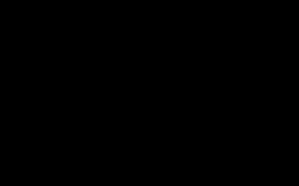
\includegraphics[width=0.50\textwidth]{LC21FieldConfig}
  \caption{\label{LC21FieldConfig}
(Color online)~~~
Discretization of a 1\dmn\ field theory.
Horizontal: $\zeit$ coordinate, with lattice sites marked by dots and
labelled by $\zeit\in\integers$.
(a)
A periodic field $\ssp(\zeit)$, plotted as a function of continuous
coordinate $\zeit$.
(b)
A corresponding discretized period-$5$ {\lattstate}
$\Xx=\cycle{\ssp_0 \ssp_1 \ssp_2 \ssp_3 \ssp_4}$,
with discretized field $\ssp_\zeit$ plotted as a bar
centred at lattice site $\zeit$.
In what follows we use `lattice units' \(a=1\).
          }
\end{figure}
%%%%%%%%%%%%%%%%%%%%%%%%%%%%%%%%%%%%%%%%%%%%%%%%%%%%%

A scalar field $\ssp(x)$ over $d$ Euclidean coordinates can be
discretized by
replacing the continuous space by a $d$\dmn\ hypercubic {integer lattice}
$\lattice$, with lattice spacing $a$, and
evaluating the {field} only on the
lattice points\rf{MonMun94,MunWal00}
\beq
\ssp_z
=
\ssp(x)
    \,,\qquad \qquad x = az= \mbox{lattice point}
    \,,\quad z \in \integers^d
\,,
\ee{LattField}
see \reffig{LC21FieldConfig}.
A given {\em field configuration} (here in one {\spt} dimension)
\beq
\Xx =
\cdots {\ssp}_{-3} {\ssp}_{-2}\,{\ssp}_{-1}\,
       {\ssp}_0\,
      {\ssp}_{1} {\ssp}_{2} {\ssp}_{3} {\ssp}_{4}  \cdots
\,,
\ee{stateSp}
taking any value in system's $\infty$\dmn\ \emph{\statesp}
$\ssp_{z}\in\reals$, occurs with probability
\beq
p(\Xx)\,=\, \frac{1}{Z}\,\e^{-\action[\Xx]}
\,,\qquad Z=Z[0]
\,.
\label{ProbConf}
\eeq
Here $Z$ is a normalization factor, given by the \emph{partition
function}, the integral over probabilities of all
configurations,
\beq
Z[\source]	% = e^{W[\source]}
    \,=\, \int d\Xx\,e^{-\action[\Xx] + \Xx \cdot \source}
    \,,\qquad
d\Xx = \prod_{z}^{\lattice} d\ssp_z
\,,
\ee{partFunct}
where $\source=\{\Ssym{z}\}$ is an external `source' that one can vary
at will, site-by-site, and $\action[\Xx]$ is the action that defines the
theory. %\rf{FieldThe}
The dimension of the partition function integral is the number of lattice
sites $N_\lattice$.
%, \ie, the lattice volume.   % =\Det\lattice$.

Motivated by WKB `semi-classical' or saddle-point
approximations\rf{gutbook} to the partition function \refeq{partFunct},
in this paper we describe their deterministic underpinning, the corresponding
\emph{deterministic} field theory, with partition function built from
solutions to the variational saddle-point condition
\beq
F[\Xx_c]_z =
\action[\Xx_c]_z - \Ssym{z} =0
\,,\qquad
\action[\Xx]_z=\frac{\delta{\action[\Xx]}}{\delta\ssp_z~}
\,,
\ee{LC21eqMotion}
with a global deterministic solution $\Xx_c$ satisfying this local extremal
condition on every lattice site.
In order to distinguish a \emph{solution} to the Euler–Lagrange equations
\refeq{LC21eqMotion} from an {arbitrary} \emph{field configuration}
\refeq{stateSp}, we refer to the solutions as
\emph{{\lattstate}s}, each a set of lattice site field values
\beq
\Xx_c = \{\ssp_z\}
\,,
\label{1dLattStat}
\eeq
that satisfies the local {condition} \refeq{LC21eqMotion} globally,
over all lattice sites.
For a finite lattice segment $\Xx$, one needs to specify the boundary
conditions ({\bcs}).
%  for the Green's function \refeq{tempCatGreen}.
The companion article \refref{GHJSC16} tackles the Dirichlet {\bcs}, a
difficult, time-translation symmetry breaking, and from the \po\ theory
perspective, a wholly unnecessary, self-inflicted pain. All that one
needs to solve the {\templatt} are the $\cl{}$-periodic,
time-translation enforced {\bcs} that we shall use here.
    \PC{2020-02-08}{
Complain about that stupidity clearly both in the intro and in conclusions.
    }
An example is the 1 {\spt} dimension \brick\ of fields of period
$\cl{}=5$ sketched in \reffig{LC21FieldConfig}\,(b),
\beq
\Xx_c = \cycle{\ssp_0 \ssp_1 \ssp_2 \ssp_3 \cdots \ssp_{\cl{}-1}}
\,,
\ee{1dLattStatC_n}
with its infinite repetition --for a sketch, see
\reffig{fig:1dLatStatC_5}\,(1)-- denoted by an overbar.
The first field value $\ssp_0$ in the \brick\ is evaluated on the lattice site 0,
the second $\ssp_1$ on the lattice site 1,
the $(\cl{}+1)$th $\ssp_{\cl{}}=\ssp_0$ on the lattice site $\cl{}$,
with $k$th lattice site field value $\ssp_{k}=\ssp_{\ell}$,
where $\ell=k$~(mod $\cl{}$).

What we call here a chaotic `field' at a discretized spacetime lattice
site $z$, a solid state physicist would call the state of a `particle' at
crystal site $z$, coupled to its nearest neighbors. A solid state
physicist endeavours to understand $N$-particle chaotic systems in
many-body or `large $N$' settings, where in practice any $N$ larger than 2
is `large'. Chaotic field theory is {\em ab initio} formulated for infinite
time and infinite space lattice, but its periodic theory description is
-thanks to hyperbolicity-- computationally powerful already for $N=2, 3,
\cdots$, where $N$ is the number of sites in Bravais cells that tile the
spacetime.

Each {\lattstate} is a distinct deterministic solution $\Xx_c$ to the
discretized Euler–Lagrange equations \refeq{LC21eqMotion}, so its
probability is a $N_\lattice$\dmn\ Dirac delta function
(that's what we mean by the system being \emph{deterministic})
\beq
p_c(\Xx)\,=\, \frac{1}{Z}\,\delta(F[\Xx_c-\Xx])
\,.
\label{DiracDeltaExp}
\eeq

% To comfort sceptics, we verify
In \refsect{s:LC21notHill} we  verify that this
definition agrees with the customary for\-ward-in-time \FP\ probability
evolution\rf{CBmeasure} (see \toChaosBook{section.19.2}{sect.~19.2}). The
new, field-theoretical formulation is vastly preferable to the
for\-ward-in-time formulation when it comes to higher \spt\
dimensions\rf{CL18}.

As is case for a WKB approximation\rf{gutbook}, the {deterministic} field
theory partition sum has support only on lattice field values that are
solutions to the variational saddle-point condition \refeq{LC21eqMotion},
and the partition function \refeq{ProbConf} is now a sum over
configuration \statesp\ \refeq{stateSp} \emph{points},
\bea
Z_c[\source] &=& \sum_c e^{N_\lattice W_c[\source]}
            \continue
e^{N_\lattice W_c[\source]}
    &=& \int_{\pS_c} d\Xx\,\delta(F[\Xx])
    \,=\, \frac{1}{\left|\Det\jMorb_c\right|}
\,,
\label{ClassPartitF}
\eea
where $\pS_c$ is a small neighborhood of  $\Xx_c$, and we refer to
the $[N_c\!\times\!N_c]$ matrix of second derivatives
\beq
(\jMorb_c)_{z'z} = \frac{\delta F[\Xx_c]_{z'}}{\delta \ssp_{z}}
             = \action[\Xx_c]_{z'z}
\ee{jacobianOrb}
as the \emph{\jacobianOrb}.

In what follows, we shall almost exclusively deal only with deterministic field
theory and omit the subscript `$c$' in $\Xx_c$ througout.

\subsection{Lattice Laplacian}
\label{s:LC21lattLap}


Let's have a look at the lattice free field theory action
\beq
\action_0[\Xx]=
          \frac{1}{2}\transp{\Xx}\left(-\Box + {\mu}^2\mathsf{1} \right)\Xx
\,,
\ee{LC21freeAction}
where the `discrete Laplace operator', `central difference operator', or
the `graph Laplacian'%
\rf{PerViv,Pollicott01,Cimasoni12,MraRin12,GodRoy13,Pozrikidis14}
\beq
\Box\,\ssp_z =
    % \frac{1}{2d}
    \sum_{||z'-z||=1} \!\! (\ssp_{z'} - \ssp_z)
 \quad \mbox{for all} \ z,z' \in \lattice % \integers^d
% \,,\quad ||i||:=\sum_{k=1}^{d}|i_k|
% \,,
\ee{LC21:Lap}
is the average of the lattice field variation $\ssp_{z'}-\ssp_z$
over the sites nearest to the site $z$.
For example, for a hypercubic lattice in one and two dimensions this
discretized Laplacian is given by
\bea
\Box\,\ssp_\zeit &=& \ssp_{\zeit+1} - 2\,\ssp_{\zeit} + \ssp_{\zeit-1}
    \label{LC21LaplTime}\\
\Box\,\ssp_{j\zeit}
     &=&
\ssp_{j,\zeit+1} + \ssp_{j+1,\zeit} - 4\,\ssp_{j\zeit}
                 + \ssp_{j,\zeit-1} + \ssp_{j-1, \zeit}
\,.
\label{LC21LaplSpaceTime}
\eea

For action \refeq{LC21freeAction} this is the discretized
{\sPe}\rf{FetWal03}, also known as the {Yukawa} or Klein–Gordon
equation, where  ${\mu}^2>0$ is the Klein–\-Gordon mass-squared.

\subsection{1\dmn\ lattice field theories}
\label{s:LC21FT1d}

Discrete time evolution is frequently recast into a 1\dmn\ temporal
lattice field theory form, essentially by anyone who rewrites a
dynamical systems discrete time evolution problem as a $k$-point recurrence,
for example in
\refrefs{FeHa82,noisy_Fred,conjug_Fred,diag_Fred}.
As already in one \spt\ dimension there is much to be learned about the
role symmetries play in solving lattice field theories, that is what we
will focus on in this paper (time-reversal
\refsects{s:latt1d}{sect:LC21Lind1d}), with the $2$\dmn\ \spt\ field
theories discussed in the sequel\rf{CL18}.

We shall consider scalar field theories of polynomial type, with a local
potential%
\rf{FriMil89,DulMei00,LiMal04,AnBoBa17,AnBoBa18,Anastassiou21}
\beq
V(\ssp_\zeit,\Ssym{\zeit}) =  \frac{g}{k}\ssp_{\zeit}^k
                            - \ssp_{\zeit}^2 -\Ssym{\zeit}\,\ssp_\zeit
\ee{polynPotent}
added to the Laplacian in \refeq{LC21freeAction} on each lattice
site $\zeit$. The discrete Euler–Lagrange equations \refeq{LC21eqMotion}
now take form of 3-term recurrence, second-order difference equations
\bea
- \ssp_{\zeit+1} + V'(\ssp_\zeit,\Ssym{\zeit}) - \ssp_{\zeit-1}
    &=&
0  % was \Ssym{\zeit}
\,.  %\qquad  \ssp_{\zeit} \in [0,1)
\label{LC21:1dTempFT}% \refeq{LC21:1dTempFT}
\eea

We start with the first order difference equation that we call
`{temporal Bernoulli}' (\refsect{s:coinToss}),
\bea
- \ssp_{\zeit+1} + {s}\,\ssp_{\zeit}
    \qquad\quad\;
    &=&
\Ssym{\zeit}
%\,,\qquad  \ssp_{\zeit} \in [0,1)\,,
\label{LC21:1dBernLatt}    % labelled {1stepDiffEq} elsewhere
\eea
in order to motivate the second-order difference
Euler–Lagrange equations \refeq{LC21:1dTempFT}
that we call, in the cases considered here,
the `{\templatt}' (\refsect{s:kickRot}),
`{\henlatt}' (\refsect{s:henlatt}), and
`temporal {$\phi^4$} theory'  (\refsect{s:phi4latt}), respectively:
\bea
- \ssp_{\zeit+1}  +  \,{s}\,\ssp_{\zeit} - \ssp_{\zeit-1}
    &=&
\Ssym{\zeit}
%\,,\qquad  \ssp_{\zeit} \in [0,1)
\label{LC21:1dTemplatt}\\
- \ssp_{\zeit+1} + {a}\,\ssp_{\zeit}^2 - \ssp_{\zeit-1}
    &=&
\Ssym{\zeit}
%\,,\qquad  \Ssym{\zeit}=2
\label{LC21:1dHenlatt}\\
- \ssp_{\zeit+1} + {g}\,\ssp_{\zeit}^3 - \ssp_{\zeit-1}
    &=&
\Ssym{\zeit}
%\,.
\label{LC21:1dPhi4}
\eea
Qualifier `temporal' is used here to emphasize that we view 1\dmn\
examples as special cases of `\spt' field theories; much of our
methodology for $d$\dmn\ deterministic field theories can be profitably
explained by working out $1$\dmn\ field theories.
Lurking here is the totality of the map-iteration dynamical systems
theory, but the reader will find it more profitable, and less confusing,
to think of these simply as lattice problems, and forget that the index
$\zeit$ often stands for `time'.

So, what is a `chaotic', or `turbulent' field theory?
As we shall see, all of the above, as well as their
higher\dmn\ \spt\ siblings are `chaotic' for sufficiently strong `stretching
parameters' or `coupling constants'  ${s}$, ${a}$ or ${g}$.
Our goal here is to make this `{\spt} chaos' tangible and precise, by
acquainting the reader what we believe are
some of the simplest, most elegant examples chaotic field theories.

\newpage % REMOVE
    % siminos/reversal/Bernoulli.tex      pdflatex LC21; bibtex LC21
% temporary: siminos/spatiotemp/chapter/LC21Bernoulli.tex
% $Author: predrag $ $Date: 2021-12-24 01:25:20 -0500 (Fri, 24 Dec 2021) $

\section{A fair coin toss}
\label{s:coinToss}
\renewcommand{\ssp}{\ensuremath{x}}               % state space point

The very simplest example of a deterministic law of evolution that gives
rise to `chaos' is the {\em Bernoulli} map, \reffig{fig:BernPart}\,(a),
which models a
\HREF{https://www.random.org/coins/?num=2&cur=40-antique.aurelian} {coin
toss}. Starting with a random initial state, the map generates,
deterministically,  a sequence of tails and heads with the 50-50\%
probability.

We introduce the model in its conventional, time-evolution dynamical
formulation, than reformulate it as a lattice field theory, solved by
enumeration of all admissible \emph{{\lattstate}s}, field configurations that
satisfy a  global fixed point condition, and use this simple setting to
motivate
(1) the \emph{fundamental fact}: for a given lattice period, the {\em
\HillDet} of stabilities of global solutions counts their number
(\refsect{sect:fundFact}), and
(2) the {\tzeta} counts their translational symmetry group orbits
(\refsect{s:zeta1D}).

\subsection{Bernoulli map} %Doubling map}
\label{s:Bernoulli}
%ChaosBook return to
% \example{Bernoulli shift map \statesp\ partition.}{ \label{exam:BernMap}

%\renewcommand{\statesp}{state space}
%\renewcommand{\Statesp}{State space}
%\renewcommand{\stateDsp}{state-space}
%\renewcommand{\StateDsp}{State-space}

%
%%%%%%%%%%%%%%%%%%%%%%%%%%%%%%%%%%%%%%%%%%%%%%%%%%%%%%%%%%%%%
\begin{figure}
  \centering
{(a)}
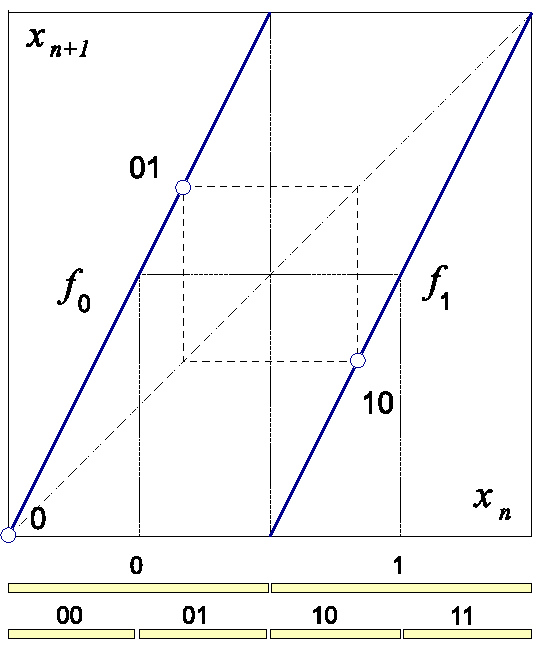
\includegraphics[width=0.35\textwidth]{BernPartCL18}
~~~
{(b)}$\!\!\!\!$
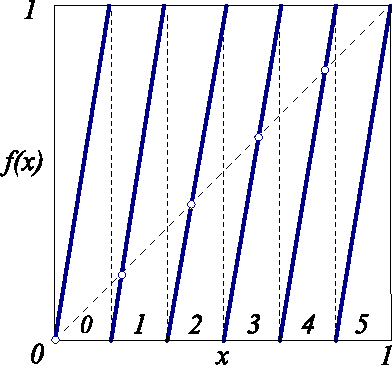
\includegraphics[width=0.40\textwidth]{fig_d_2CL18}

  \caption{\label{fig:BernPart}
(Color online)~~~
(a)
The `coin toss' map \refeq{BerShift}, together with the
$\cycle{0}$ fixed point, and the \cycle{01} 2-cycle. Preimages
of the critical point $\ssp_c=1/2$ partition the unit interval into
$\{\pS_0,\pS_1\}$, $\{\pS_{00},\pS_{01},\pS_{10},\pS_{11}\}$, $\dots$,
subintervals.
(b)
The base-${s}$ Bernoulli map, here with the `dice throw' stretching parameter ${s}=6$,
partitions the unit interval into $6$ subintervals $\{\pS_{\Ssym{}}\}$,
labeled by the ${6}$-letter alphabet \refeq{base-sAlph}. As the map is a
circle map, $\ssp_{5}=1=0=\ssp_{0} \quad(\mbox{mod}\;1)$.
          }
\end{figure}
%%%%%%%%%%%%%%%%%%%%%%%%%%%%%%%%%%%%%%%%%%%%%%%%%%%%%%%%%%%%%%
%

The base-2 {\em Bernoulli} shift map,
\index{Bernoulli!shift}
\index{shift!Bernoulli}
\beq
\ssp_{\zeit+1} =
% \flow{}{\ssp_{\zeit}} =
\left\{ \begin{array}{ll}
        f_0(\ssp_{\zeit}) =  2 \ssp_{\zeit} \,, \quad
                                    & \ssp_{\zeit} \in \pS_0=[0,1/2) \\
        f_1(\ssp_{\zeit}) =  2 \ssp_{\zeit} \;\; (\mbox{mod}\;1)\,, \quad
                                    & \ssp_{\zeit} \in \pS_1 =[1/2,1)
         \end{array}\right.
\,,
\ee{BerShift}
is shown in \reffig{fig:BernPart}\,(a).
If the linear part of such map has an integer-valued slope,
or `stretching' parameter $s\geq2$,
\beq
\ssp_{\zeit+1} \,=\, {s} \ssp_{\zeit}
\ee{BerStretch}
that maps state $\ssp_{\zeit}$ into a state in the `extended \statesp',
outside the unit interval,
the $(\mbox{mod}\;1)$ operation results in the base-${s}$ Bernoulli
circle map,
\renewcommand{\ssp}{\ensuremath{\phi}}             % lattice site field
\beq
\ssp_{\zeit+1}
% = \flow{}{\ssp_{\zeit}}
= {s} \ssp_{\zeit}
\;\; (\mbox{mod}\;1)
%    \,,\qquad \qquad \ssp_{\zeit}\in [0,1)
\,,
\ee{n-tuplingMap}
sketched as a \HREF{https://www.random.org/dice/}{dice throw} in
\reffig{fig:BernPart}\,(b).
The $(\mbox{mod}\;1)$ operation subtracts
$\Ssym{\zeit}=\left\lfloor{s}\ssp_{\zeit}\right\rfloor$, the integer part of ${s}
\ssp_{\zeit}$, or the circle map \emph{winding number}, to keep
$\ssp_{\zeit+1}$ in the unit interval $[0,1)$, and partitions the unit
interval into ${s}$ subintervals $\{\pS_\Ssym{}\}$,
\beq
\ssp_{\zeit+1}
% = \flow{}{\ssp_{\zeit}}
% = \hflow{}{\ssp_{\zeit}} - \Ssym{\zeit+1}
= {s} \ssp_{\zeit} - \Ssym{\zeit}
\,,\qquad  \ssp_{\zeit}\in\pS_{\Ssym{\zeit}}
\,,
\ee{circ-m}
where $\Ssym{\zeit}$ takes values in the ${s}$-letter alphabet
\beq
\Ssym{} \in \A=\{0,1,2,\cdots,s-1\}
\,.
\ee{base-sAlph}

The Bernoulli map is a highly instructive example of a
hyperbolic dynamical system. Its symbolic dynamics is simple:
the base-${s}$ expansion of the initial point $\ssp_0$ is also its
temporal itinerary, with symbols from alphabet \refeq{base-sAlph}
indicating that at time $\zeit$ the orbit visits the subinterval
$\pS_{\Ssym{\zeit}}$. The map is a `shift':
a multiplication by ${s}$ acts on the base-${s}$
representation of $\ssp_{0}=.\Ssym{1}\Ssym{2}\Ssym{3}\cdots $ (for
example, binary, if ${s}=2$) by shifting its digits,
\bea
\ssp_{1}
    &=& \map(\ssp_{0})
    =.\Ssym{2}\Ssym{3}\cdots
%\continue
%\ssp_{\Ssym{2}\Ssym{3}\cdots}
%    &=& \shift{}\,\ssp_{\Ssym{1}\Ssym{2}\Ssym{3}\cdots}
\,.
\label{shiftBern}
\eea

Periodic points can be counted by observing that the preimages of
critical points $\{\ssp_{c1},\ssp_{c2},\cdots\ssp_{c,s-1}\}$ =
$\{{1}/s,{2}/s,\cdots,(s-1)/s\}$ partition the unit interval into
$\{\pS_0,\pS_1,\cdots,\pS_{s-1}\}$, $\{\pS_{\Ssym{1}\Ssym{2}}\}$, $\dots$,
$s^\cl{}$ subintervals, each containing {\em one}  unstable
period-$\cl{}$ periodic point
$\ssp_{\Ssym{1}\Ssym{2}\cdots\Ssym{\cl{}}}$, with stability multiplier
${s}^\cl{}$, see \reffig{fig:BernPart}. The Bernoulli map is a
full shift, in the sense that every itinerary is \admissible, with one
exception: on the circle, the rightmost fixed point is the same as the
fixed point at the origin, $\ssp_{s-1}=\ssp_{0}\quad(\mbox{mod}\;1)$,
so these fixed points are identified and counted as one, see
\reffig{fig:BernPart}. The total number of periodic points of period
$\cl{}$ is thus
\beq
N_{\cl{}} = s^{\cl{}} - 1
\,.
\ee{noPerPtsBm}


\subsection{Temporal Bernoulli}
\label{s:1D1dLatt}

To motivate our formulation of a \spt\ chaotic field theory to be
developed below, we now recast the local initial value, time-evolution
Bernoulli map problem as a \emph{temporal lattice} fixed point condition,
the problem of enumerating and determining all global solutions.

`Temporal' here refers to the lattice site field  $\ssp_\zeit$ and the
source (winding number) $\Ssym{\zeit}$ taking their values on the lattice
sites of a 1\dmn\ \emph{temporal} integer lattice $\zeit\in\integers$.
Over a finite lattice segment, these can be written compactly  as a
\emph{{\lattstate}} and the corresponding \emph{symbol \brick}
\beq
\transp{\Xx} % = \{\ssp_j\}
             = (\ssp_{\zeit+1},\cdots,\ssp_{\zeit+\cl{}})
\,,\quad
\transp{\Mm} % = \{\Ssym{j}\}
             = (\Ssym{{\zeit+1}},\cdots,\Ssym{{\zeit+\cl{}}})
\,,
\ee{pathBern}
where $\transp{(\cdots)}$ denotes a transpose.
The Bernoulli equation \refeq{circ-m}, rewritten as a first-order
difference equation
% \refeq{LC21:1dBernLatt}
\beq
-\ssp_{\zeit+1} + {s}\ssp_{\zeit} = \Ssym{\zeit}
\,,\qquad  \ssp_{\zeit} \in [0,1)
\,,
\ee{1stepDiffEq}  % called {...1dBernLatt} elsewhere
takes the matrix form
\beq
\jMorb\,\Xx =  \Mm
\,,\qquad
\jMorb =  - {\shift} + {s}\id
% former \ee{tempBernFix}
\,,
\ee{tempBern}
where the $[\cl{}\!\times\!\cl{}]$ matrix
\beq
\shift_{jk}=\delta_{j+1,k}
\,,\qquad
\shift
=  \left(\begin{array}{ccccc}
             0    &  1    &        &   &  \cr
                  &  0    &   1    &   &  \cr
                  &       &        & \ddots &  \cr
                  &       &        & 0 & 1 \cr
             1    &       &        &   & 0
          \end{array} \right)
\,,
\ee{hopMatrix}
implements the shift operation \refeq{shiftBern}, a cyclic permutation
that translates forward-in-time {\lattstate} $\Xx$ by one site,
$\transp{(\shift \Xx)}=(\ssp_2,\ssp_3,\cdots,\ssp_\cl{},\ssp_1)$. The
time evolution law \refeq{circ-m} must be of the same form for all times,
so the {\shiftOp} $\shift$ has to be time-translation invariant, with
$\shift_{\cl{}+1,\cl{}}=\shift_{1\cl{}}=1$ matrix element enforcing the
periodicity. After $\cl{}$ shifts, a {\lattstate} returns to the initial
state,
\beq
\shift^\cl{}=\id
\,.
\ee{shift2n}

As the {temporal Bernoulli} condition \refeq{tempBern} is a linear
relation, a given \brick\ $\Mm$, or `code' in terms of alphabet
\refeq{base-sAlph}, corresponds to a unique temporal {\lattstate} $\Xx$.
That is why Percival and Vivaldi\rf{PerViv} refer to such symbol \brick\
$\Mm$ as a {\em linear code}.

\subsection{Bernoulli as a continuous time dynamical system}
\label{s:bernODE}

The discrete time derivative of a lattice configuration \Xx\ evaluated at the
lattice site \zeit\ is given by the {difference operator}\rf{Elaydi05}
    \index{lattice!derivative}\index{derivative, lattice}
    \index{lattice!derivative, forward}\index{difference operator}
\beq
\dot{\Xx}_\zeit =
\left[\frac{\partial\Xx}{\partial\zeit}\right]_\zeit
        =
    \frac{\ssp_{\zeit+1} - \ssp_{\zeit}}{\Delta\zeit}
\,.
\ee{lattTimeDer}
The {temporal Bernoulli} condition \refeq{tempBern} %{1stepDiffEq}
can be thus viewed as a time-discretized, first-order ODE dynamical
system
\beq
   \dot{\Xx} \,=\, \vel(\Xx) \,,
\ee{1stepVecEq}
where the `velocity' vector field $\vel$ is given by
\[
\vel(\Xx) \,=\,
   % \vel(\Xx;\Mm) \,=\,
(s-1)\,\Xx-\Mm
\,,
\]
with the time increment set to $\Delta\zeit=1$, and perturbations that
grow (or decay) with rate $({s}-1)$. By inspection of
\reffig{fig:BernPart}\,(a), it is clear that for \emph{shrinking},
${s}<1$  parameter values the orbit is stable forward-in-time, with a
single linear branch, 1-letter alphabet $\A=\{0\}$, and the only
{\lattstate}s being the single fixed point  $\ssp_0=0$, and its repeats
$\Xx=(0,0,\cdots,0)$. However, for \emph{stretching},  ${s}>1$  parameter
values, the Bernoulli system (more generally, R{\'e}nyi's beta
transformations\rf{Renyi57}) that we study here, every {\lattstate}
$\Xx_\Mm$ is unstable, and there is a {\lattstate} for each admissible
symbol \brick\ \Mm.
    %
    \PC{2021-08-23} {
    Should we include ``Quotienting the temporal Bernoulli system''
    \refeq{1stepDiffEqBlog}?
    }


\bigskip

\noindent\textbf{A fair coin toss, summarized.}
We refer to the \emph{global} temporal lattice condition \refeq{tempBern}
as the `\emph{temporal} Bernoulli', in order to distinguish it from the
one-time step Bernoulli evolution \emph{map} \refeq{n-tuplingMap}, in
preparation for the study of \emph{\spt} systems to be undertaken in
\refref{CL18}. In the lattice formulation, a \emph{global} {temporal
{\lattstate}} $\Xx_\Mm$ is determined by the requirement that the
\emph{local} temporal lattice condition \refeq{1stepDiffEq} is satisfied
at every lattice site. In \spt\ formulation there is no need for
forward-in-time, close recurrence searches for the returning periodic
points. Instead, one determines each global {temporal {\lattstate}}
$\Xx_\Mm$ at one go, by solving the fixed point condition
\refeq{tempFixPoint}, and one determines the total number of
{\lattstate}s by computing the {\HillDet} \refeq{detBern0} of the
\emph{\jacobianOrb}. The most importantly for what follows, the \spt\
field theory of \refref{CL18}, this calculation requires no recourse to any
\emph{explicit coordinatization and partitioning of system's state
space}, and \emph{no explicit symbolic dynamics}.
    \PC{2020-12-17}{
Link to the ChaosBook. Maybe refer to \AW.
    }

%%%%%%%%%%%%%%%%%%%%%%%%%%%%%%%%%%%%%%%%%%%%%%%%%%%%%%%%%%%%%%%%%%%%%%%
%\renewcommand{\statesp}{phase space}
%\renewcommand{\Statesp}{Phase space}
%\renewcommand{\stateDsp}{phase-space}
%\renewcommand{\StateDsp}{Phase-space}

    % siminos/reversal/cat.tex      pdflatex LC21; bibtex LC21
% temporary: siminos/spatiotemp/chapter/LC21cat.tex
% $Author: predrag $ $Date: 2021-12-24 01:25:20 -0500 (Fri, 24 Dec 2021) $

\section{A kicked rotor}
\label{s:kickRot}

Temporal Bernoulli is the simplest example of a chaotic lattice field
theory. Our next task is to formulate a deterministic {\spt}ly chaotic
field theory, Hamiltonian and energy conserving, because (a) that is
physics, and (b) one cannot do quantum theory without it. We need a
system as simple as the Bernoulli map, but mechanical. So, we move on
from running in circles, to a mechanical rotor to kick.

The 1-degree of freedom maps that describe kicked rotors
subject to discrete time sequences of angle-dependent force pulses
$P(\coord_{\zeit})$, $\zeit\in\integers$,
\bea
\coord_{\zeit+1} &=& \coord_{\zeit} + p_{\zeit+1} \qquad  (\mbox{mod}\;1),
    \label{LC21PerViv2.1b}\\
p_{\zeit+1}       &=& p_{\zeit} + P(\coord_{\zeit})
\,,
    \label{LC21PerViv2.1a}
\eea
with $2\pi \coord$ the  angle of the rotor, $p$ the momentum conjugate to
the angular coordinate $\coord$, and the angular pulse
$P(\coord_{\zeit})=P(\coord_{\zeit+1})=-V'(\coord_{\zeit})$ lattice
periodic with period $1$, play a key role in the theory of deterministic
and quantum chaos in  atomic physics, from the Taylor, Chirikov and
Greene  standard map\rf{Lichtenberg92,Chirikov79}, to the cat maps that
we turn to now. The equations are of the Hamiltonian form:
eq.~\refeq{LC21PerViv2.1b} is $\dot{\coord}=p/m$ in terms of discrete
time derivative \refeq{lattTimeDer}, \ie, the configuration trajectory
starting at $\coord_{\zeit}$ reaches
$\coord_{\zeit+1}=\coord_{\zeit}+p_{\zeit+1}\Delta{\zeit}/m$ in one time
step $\Delta{\zeit}$. Eq.~\refeq{LC21PerViv2.1a} is the time-discretized
$\dot{p}=-\partial V(\coord)/\partial \coord$: at each kick the angular
momentum $p_{\zeit}$ is accelerated to $p_{\zeit+1}$ by the force pulse
$P(\coord_{\zeit})\Delta{\zeit}$, with the time step and the rotor mass
set to $\Delta{\zeit}=1$,  $m=1$.

%\section{Life of a single Hamiltonian cat}
\subsection{Cat map}
%    \fi
\label{s:catPV}

The simplest kicked rotor is subject to force pulses
$P(\coord)={\mu}^2\coord$ proportional to the angular displacement
$\coord$: in that case, the map
(\ref{LC21PerViv2.1b},\ref{LC21PerViv2.1a}) is of form
%    \PC{2021-12-26}{I see \refeq{HLHamiltonsEquations} here:)}
 \beq
 \left(\begin{array}{c}
 \coord_{\zeit+1}  \\
   p_{\zeit+1}
  \end{array} \right )=
  \jMat \left(\begin{array}{c}
 \coord_{\zeit}  \\
   p_{\zeit}
  \end{array} \right )\quad (\mbox{mod}\;1)
    \,,  \qquad
 {\jMat} =\left(\begin{array}{cc}
 {\mu}^2+1 & 1 \\
  {\mu}^2 & 1
  \end{array} \right)
\,.
\ee{catMap}
The $(\mbox{mod}\;1)$ makes the map a
discontinuous `sawtooth,' unless ${\mu}^2$ is a positive integer.
The map is then a Continuous Automorphism of the Torus
known as the Thom-Anosov-Arnol'd-Sinai
{\em `cat map'}\rf{ArnAve,deva87,StOtWt06}, extensively studied as the
simplest example of a chaotic Hamiltonian system.

The determinant of the one-time-step Jacobian is
$\det \jMat=1$, \ie, the mapping is area-preserving.
Let ${s}=\tr{\jMat}={\mu}^2+2$ be the trace of the Jacobian.
For $|s|>2$ the $\jMat$ {characteristic equation}
\beq
\ExpaEig^{2} - {s}\ExpaEig + 1 = 0
\,,
\ee{LC21:StabMtlpr}
has real roots
$(\ExpaEig\,,\;\ExpaEig^{-1})$  and a positive Lyapunov exponent
$\Lyap >0$,
\beq
\ExpaEig=e^{\Lyap} = \frac{1}{2}(s+\sqrt{(s-2)(s+2)})
\,,\qquad
{s}=\tr{\jMat}=\ExpaEig+\ExpaEig^{-1}
\,.
\ee{StabMtlpr}
The eigenvalues are functions of the stretching parameter $s$, and
for $|s| > 2$ the cat map \refeq{catMap} is a fully chaotic
Hamiltonian dynamical system.

\subsection{\tempLatt}
\label{s:catLagrange}
    % earlier names:
    % \section{Life of a single Lagrangian cat}
    % \section{Cat map in Lagrangian formulation}
\renewcommand{\period}[1]{{\ensuremath{n_{#1}}}}
    % discrete length of a cycle, Predrag

In order to motivate our formulation of higher-dimensional \spt\ chaotic
field theories, to be developed in \refref{CL18}, we now recast the
\emph{local} initial value, Hamiltonian time-evolution  as a
\emph{global} solution to the Euler–Lagrange equations.

The 2-component field at the
temporal lattice site \zeit,
\(
\ssp_{\zeit} =(\coord_{\zeit},p_{\zeit}) \in  (0,1]\times(0,1]
\)
is kicked rotor's the angular position and momentum.
Hamilton's equations (\ref{LC21PerViv2.1b},\ref{LC21PerViv2.1a}) induce
for\-ward-in-time evolution on a 2-torus  $(\coord_{\zeit},p_\zeit)$ {\em
phase space}.
Eliminating the momentum by Hamilton's discrete time velocity
eq.~\refeq{LC21PerViv2.1b},
\beq
(\coord_\zeit,p_\zeit) =
\left(
    \coord_{\zeit},\frac{\coord_{\zeit} - \coord_{\zeit-1}}{\Delta\zeit}
\right)
%\,,\qquad \Delta\zeit= 1
\,,
\ee{Ham2Lagr}
setting the time step to $\Delta\zeit=1$, and forgetting for a moment
the $(\mbox{mod}\;1)$ condition, the
for\-ward-in-time Hamilton's first order difference equations are brought
to the second order difference, 3-term recurrence Euler–Lagrange equations
for scalar field $\ssp_{\zeit}=q_\zeit$,
\beq
\ssp_{\zeit+1} - 2\,\ssp_{\zeit} + \ssp_{\zeit-1} = P(\ssp_{\zeit})
\,.
\ee{cattyMappo}
But that is Newton's Second Law: ``acceleration equals
force,'' so Percival and Vivaldi\rf{PerViv} refer to this formulation as
`Newtonian'. Here we follow Allroth\rf{Allroth83}, Mackay, Meiss,
Percival, Kook \& Dullin\rf{MacMei83,meiss92,MKMP84,DulMei98,kooknewt},
and Li and Tomsovic\rf{LiTom17b} in referring  to it as `Lagrangian'.

For the cat map \refeq{catMap}, the Lagrangian passage
\refeq{Ham2Lagr} to the  scalar field  $\ssp_{\zeit}$ leads to the \PV\
`two-configuration representation'\rf{PerViv}
\beq
 \left(\begin{array}{c}
 \ssp_{\zeit}  \\
 \ssp_{\zeit+1}
 \end{array} \right )=
 \jMat_{PV} \left(\begin{array}{c}
 \ssp_{\zeit-1}  \\
 \ssp_{\zeit}
 \end{array} \right ) %\mbox{ mod } 1
 - \left(\begin{array}{c}
 0  \\
 \Ssym{\zeit}
 \end{array} \right )
 \,,  \qquad
 {\jMat_{PV}} =\left(\begin{array}{cc}
 0 & 1 \\
 -1 & s
 \end{array} \right ),
%\,.
\ee{LC21PerViv}
with matrix $\jMat_{PV}$ acting on the 2\dmn\ space of successive
configuration points $\transp{(\ssp_{\zeit-1},\ssp_{\zeit})}$. As was
case for the Bernoulli map \refeq{1stepDiffEq}, the cat map
$(\mbox{mod}\;1)$ condition \refeq{catMap} is enforced by integers
$\Ssym{\zeit}\in  \A$, where for a given integer stretching parameter $s$
the alphabet \A\ ranges over $|\A|={s}\!+\!1$ possible values for
$\Ssym{\zeit}$,
\beq
\A=\{\underline{1},0,\dots s\!-\!1\}
\,,
\ee{catAlphabet}
necessary  to keep $\ssp_{\zeit}$ for all times $t$ within the unit
interval $[0,1)$. (We find it convenient to have symbol
$\underline{\Ssym{}}{}_{\zeit}$ denote $\Ssym{\zeit}$ with the negative
sign, \ie, `$\underline{1}$' stands for symbol `$-1$'.)


Written out as a second-order difference equation, the \PV\ map
\refeq{LC21PerViv} takes a particularly elegant form, that we shall
refer to as the {\em \templatt} \refeq{LC21:1dTemplatt},
\beq
-\ssp_{\zeit+1}  +  s \, \ssp_{\zeit} - \ssp_{\zeit-1}
    =
\Ssym{\zeit}
\,,
\ee{catMapNewt}
or,
in terms of a {{\lattstate}} $\Xx$, the corresponding {symbol \brick}
$\Mm$ \refeq{pathBern}, and the $[\cl{}\!\times\!\cl{}]$ {\shiftOp}
$\shift$ \refeq{hopMatrix},
\beq
(-\shift + s\id - \shift^{-1})\,\Xx =  \Mm
\,,
\ee{catTempLatt}
very much like the {temporal Bernoulli} condition \refeq{tempBern}, and
the winding numbers (sources) $\Mm$ taking their values on the lattice
sites of a 1\dmn\ \emph{temporal} lattice $\zeit\in\integers$.
%    \PC{2021-10-13}{Dropped:
%Nonlinearity of the \catlatt\ arises from restricting the admissible
%values of fields $\ssp_z$ to the unit interval.
%    }

As was the case for {temporal Bernoulli} \refeq{tempBern}, the condition
\refeq{LC21PerViv} is a linear relation: a given `code'
$\{\Ssym{\zeit}\}$ in terms of alphabet \refeq{catAlphabet} corresponds
to a unique temporal sequence $\{\ssp_\zeit\}$. That is why Percival and
Vivaldi\rf{PerViv} refer to such symbol \brick\ $\Mm$ as a {\em linear
code}. As for the Bernoulli system, $\Ssym{\zeit}$ can also be
interpreted as `winding numbers'\rf{Keating91}, or, as they shepherd
stray points back into the unit torus, as `stabilising
impulses'\rf{PerViv}. Here we use the field-theoretical parlance,
and refer to them  as `sources'.

The lattice formulation \refeq{catMapNewt} lends itself immediately to
$d$\dmn\ generalizations. An example is the Gutkin and
Osipov\rf{GutOsi15} \catlatt\ in  $d=2$ dimensions\rf{CL18}, an Arnold
cat map-inspired Euclidean scalar field theory  of form
\refeq{LC21freeAction} for which the Euler–\-Lagrange equation
\refeq{LC21eqMotion} is a 5-term recurrence relation
\beq
      -\ssp_{j,\zeit+1} - \ssp_{j,\zeit-1}
+ 2{s}\,\ssp_{j\zeit}
     - \ssp_{j+1,\zeit} - \ssp_{j-1, \zeit}
     =  \Ssym{j\zeit}
\,,
\ee{CatMap2d}
where we refer to parameter ${s}$, related to the Klein-Gordon mass in
\refeq{LC21freeAction} by ${\mu}^2=d({s}-2)$, as the `stretching
parameter'.


\subsection{\tempLatt\ as a continuous time dynamical system}
\label{s:tempCatODE}

Recall that the Bernoulli first-order difference equation could be viewed as
a time-discretization of the first-order linear ODE \refeq{1stepVecEq}. The
second-order difference equation \refeq{catMapNewt} can be interpreted as the
second order discrete time derivative ${d^2}/{dt^2}$, or the temporal
lattice Laplacian \refeq{LC21LaplTime},
\beq
\Box\,\ssp_\zeit \equiv
\ssp_{\zeit+1} - 2\ssp_{\zeit} + \ssp_{\zeit-1}
= (s-2)\ssp_{\zeit} -\Ssym{\zeit}
\,,
\ee{LC21PerViv2.2}
 with the time step set to $\Delta\zeit=1$.
In other words, if we include the cat map forcing pulse
\refeq{LC21PerViv2.1a}
\(
P(\ssp_\zeit)= - V'(\ssp_\zeit) = - (s-2)\,\ssp + \Ssym{\zeit}
\)
into the definition of
the on-site potential \refeq{LC21:1dTempFT},
\beq
V(\Xx,\Mm) = \sum_{\zeit\in\lattice}\left(
\frac{1}{2}\mu^2\ssp_\zeit^2 -\Ssym{\zeit}\,\ssp_\zeit\right)
\,,
\ee{templattV}
the force
is linear in the angular displacement $\ssp$, so
the \templatt\ Euler-Lagrange equation takes form (see free action
\refeq{LC21freeAction})
\beq
(-\Box + {\mu}^2\id)\,\Xx = \Mm
%\,,  \qquad
%{\mu}^2={s}-2
% \Box\,\ssp_{\zeit}:= \ssp_{\zeit-1}-2\ssp_{\zeit} +\ssp_{\zeit+1}
\,,
\ee{OneCat}
where the Klein-Gordon mass ${\mu}$ is related to the cat-map
stretching parameter ${s}$ by ${\mu}^2={s}-2$.

For small stretching parameter values, $s<2$, this discretized
Euler–\-Lagrange equation \refeq{LC21eqMotion} describes a set of coupled
penduli, with oscillatory solutions, known as the discrete Helmholtz
equation in applied math\rf{DiHaHu01,Lick89,FetWal03}, as  the
tight-binding model, the Harper's or Azbel-Hofstadter model in solid
state physics\rf{Peierls33,MiDuWh92,Cserti00,Economou06,CsSzDa11},  and
the critical almost Mathieu operator in mathematical physics\rf{Simon82},
with quadratic action \refeq{LC21freeAction} written as Hamiltonian
\[ %beq
H=\sum_\ell\ket{\ell}\epsilon_0\bra{\ell}
  + \sum_{\ell m}\ket{\ell}V_{\ell m}\bra{m}
\,,\quad
   V_{\ell m} = \left\{
     \begin{array}{ll}
         V & \mbox{if\ } \ell,m \mbox{ nearest neighbors}\\
         0 & \mbox{otherwise}
     \end{array}
             \right.
\] %ee{Economou06(5.7)}
with the stretching factor ${s}=-\epsilon_0/V$ in
\refeq{LC21PerViv2.2}.
%{OneCat}.

Here we study the strong stretching, $s>2$ case, known as the discrete
\sPe\rf{Dorr70,GoVanLo96,HuCon96,HuRyCo98,FetWal03,Pozrikidis14},
whose solutions are hyperbolic. We refer to the
Euler–\-Lagrange equation
\refeq{OneCat} as the `{\em \templatt}', both to distinguish it from
the for\-ward-in-time Hamiltonian cat \emph{map} \refeq{catMap}, and in the
anticipation of the \emph{\catlatt} to be discussed in the sequel
\refref{CL18}. {\catLatt} differs from all of the above models because the
field $\ssp_\zeit$ compactification to unit circle makes it a
strongly nonlinear deterministic field theory, with nontrivial symbolic
dynamics.

\bigskip

\noindent\textbf{\tempLatt, summarized.}
In the \spt\ formulation a \emph{global} {temporal {\lattstate}}
\beq
\transp{\Xx} % = \{\ssp_j\}
             = (\ssp_\zeit,\ssp_{\zeit+1},\cdots,\ssp_{\zeit+k})
\ee{path}
is not determined by a for\-ward-in-time `cat map' evolution
\refeq{catMap}, but rather by the fixed point condition
\refeq{LC21eqMotion}
% tempCatFixPoint}
that the \emph{local}, 3-term discrete temporal lattice Euler–Lagrange
equations \refeq{catMapNewt} are satisfied at every lattice point. This
temporal 1\dmn\ lattice reformulation is the bridge that takes us from
the single cat map \refeq{catMap} to the higher-\dmn\ coupled
``multi-cat'' \spt\ lattices\refrefs{GutOsi15,GHJSC16,CL18}.

And, did you know that the cute Arnold cat is but the % very fundamental
{\sPe} in disguise? And that the lattice form \refeq{catMapNewt}
of the theory is so much more elegant than the
cat-map form \refeq{catMap}?
A cat is Hooke's wild, `anti-harmonic' sister.
For $s<2$ Hooke rules: restoring oscillations around the sleepy resting
state.
For $s>2$ cats rule: exponential runaway, wrapped globally around a
\statesp\ torus. {Cat} is to {chaos} what {harmonic oscillator} is to
{order}. There is no more fundamental example of chaos in mechanics.


\renewcommand{\period}[1]{{\ensuremath{T_{#1}}}}         %continuous cycle period

    % siminos/reversal/LC21nonlinFT.tex      pdflatex LC21; bibtex LC21
% temporary: siminos/spatiotemp/chapter/LC21nonlinFT.tex
% $Author: predrag $ $Date: 2021-12-24 01:25:20 -0500 (Fri, 24 Dec 2021) $

% was \section{Nonlinear lattice field theories}
%\label{s:nonlinFT}

\section{A $\ssp^3$ field theory}
% was {{\Henlatt}}
\label{s:henlatt}

The `mod~1' in the definition of the `linear' kicked rotor, the cat map
\refeq{catMap}, makes cat map a highly nonlinear, discontinuous map. In
contrast, field theory action $\action[\Xx]$ is typically polynomial and
smooth. The simplest such nonlinear action turns out to correspond to the
paradigmatic dynamicist's model of a 2\dmn\ nonlinear dynamical system,
the {\HenonMap}\rf{henon}
\bea
    x_{\zeit+1} &=& 1-a\,x_{\zeit}^2 + b\,y_{\zeit}
        \continue
    y_{\zeit+1} &=& x_{\zeit}
\,.
\label{LC21eq2.1}
\eea
For the contraction parameter value $b=-1$ this is a Hamiltonian map.

The \emph{temporal evolution} \jacobianM\ for the $n$th iterate of the
Hamiltonian {\HenonMap} is the product of consecutive  one time-step
\jacobianMs
\beq
\jMps^\cl{}(x_0,y_0) =
\prod_{m=\cl{}-1}^{0}
            \left(\begin{array}{cc}
                -2a\,x_m & -1 \\
                         1 & 0
            \end{array}\right)
\,,\qquad x_m = \map^{m}_1 (x_0,y_0)
\,,
\ee{Henlatt-e_her}
where the successive 1-time step \jacobianMs\ are multiplied in the order
they are applied, as
$\jMps^\cl{}(x_0)=\jMps(x_{\cl{}-1})\cdots\jMps(x_0)$. So, once we have a
{\HenonMap} {\po}, we also have its Floquet
(monodromy) matrix. When $\jMps^\cl{}$ is
hyperbolic, only the expanding
eigen\-value $\ExpaEig_1=1/\ExpaEig_2$ needs to be determined, as the
determinant of the {\Henon} 1-time step \jacobianM\ is unity,
\beq
\det\jMps = \ExpaEig_1 \ExpaEig_2 = 1
\,.
\ee{LC21:HenDet}
The map is Hamiltonian in the sense that it preserves areas in the
$[x,y]$ plane.


The {\HenonMap} is the simplest map that captures chaos that arises from
the smooth stretch \& fold dynamics of nonlinear {\PoincMap}s of flows
such as R\"ossler\rf{ross}.
Written as a  2nd-order inhomogeneous difference equation\rf{DulMei00},
\refeq{LC21eq2.1} takes the
{\em \henlatt} 3-term recurrence form, explicitly time-translation
and time-reversal invariant Euler–Lagrange equation
% \refeq{LC21:1dHenlatt}:
\beq
-\ssp_{\zeit+1} + {a}\,\ssp_{\zeit}^2 - \ssp_{\zeit-1} = 1
\,.
\ee{LC21:2-step}
Just as the kicked rotor (\ref{LC21PerViv2.1b},\ref{LC21PerViv2.1a}), the map can
be interpreted as a kicked driven anaharmonic oscillator\rf{Heagy92},
with the nonlinear, cubic Biham-Wenzel\rf{afind} lattice site potential
\refeq{polynPotent}
\beq
V(\ssp_\zeit,\Ssym{\zeit}) =  \frac{a}{3}\ssp_{\zeit}^3
                            - \ssp_{\zeit}^2 -\Ssym{\zeit}\,\ssp_\zeit
    \,,\qquad
        \Ssym{\zeit} = -1
\,,
\ee{LC21BWcubic}
giving rise to kicking pulse \refeq{LC21PerViv2.1a}, so we
refer to this field theory as $\ssp^3$ theory.

Thus the lattice site field values of this $\phi^3$ theory are in
one-to-one correspondence to the unimodal \HenonMap\
Smale horseshoe repeller, cleanly split into the `left', positive stretching and
`right', negative stretching lattice site field values.
Devaney, Nitecki, Sterling and Meiss\rf{Devaney79,StMeiss98,SteDuMei99}
have shown that the Hamiltonian {\HenonMap} has a complete Smale
horseshoe for sufficiently large `stretching parameter' values
\beq
      a > 5.699310786700\cdots
\;.
\ee{LC21:SterlHen}
In numerical\rf{ChaosBook} and analytic\rf{EndGal06} calculations we fix
(arbitrarily) the stretching parameter value to $a=6$, in order to
guarantee that all $2^\cl{}$ periodic points  $\ssp=\flow{\cl{}}{\ssp}$
of the {\HenonMap} \refeq{LC21eq2.1} exist, see \reftab{tab:LC21HamHenon}.
The symbolic dynamics is as simple as the temporal Bernoulli, in contrast to the
\templatt\ which has nontrivial pruning, see \reftab{tab:catMapN_n-s=3}.


\section{A {$\phi^4$} field theory}
\label{s:phi4latt}

If a potential that is bounded from below is needed to make sense of the
probabilistic interpretation of the configuration weight
\refeq{ProbConf}, or a symmetry forbids the odd-power potentials such as
\refeq{LC21BWcubic}, one starts instead with a quartic potential
\refeq{polynPotent}
\beq
V(\ssp_\zeit,\Ssym{\zeit}) =  \frac{g}{4}\ssp_{\zeit}^4
                            - \ssp_{\zeit}^2 -\Ssym{\zeit}\,\ssp_\zeit
\,,
\ee{LC21phi4pot}
leading to an example of the `{$\phi^4$} lattice field theory'.
\refeq{LC21:1dPhi4},
\bea
- \ssp_{\zeit+1} + {g}\,\ssp_{\zeit}^3 - \ssp_{\zeit-1}
    &=&
\Ssym{\zeit}
\,.
\label{LC21:1dPhi4a}
\eea
Topology of the \statesp\ of $\phi^4$ theory is
very much like
what we had learned for the unimodal \HenonMap\ $\phi^3$ theory,
except that the repeller set is now bimodal. As long as coupling $g$
is sufficiently large, the repeller is a full 3-letter shift.
Indeed, while Smale's first horseshoe\rf{smale}, his fig.~1, was unimodal, he
also sketched the $\phi^4$ bimodal repeller, his fig.~5.

As $\phi^4$ example adds little to understanding
over what is learned from \henlatt, we will not discus is further in this
paper.


\section{Computing {\lattstate}s for nonlinear theories}
\label{s:nonlinLattStates}

Unlike the {temporal Bernoulli} \refeq{LC21:1dBernLatt} and the
{\templatt} \refeq{LC21:1dTemplatt}, for which the {\lattstate} fixed
point condition \refeq{LC21eqMotion}
% {tempCatFixPoint}
is linear and easily solved, for
nonlinear lattice field theories the {\lattstate}s are roots of
polynomials of arbitrarily high order. While Gallas and collaborators%
\rf{EndGal01,EndGal02,EG05,EG05a,EndGal06,Gallas18,Gallas20,Gallas20a}
have developed a powerful theory that yields {\HenonMap} {\po}s in
analytic form, it would be unrealistic to demand such explicit solutions for
general field theories on multi-dimensional lattices. We take a
pragmatic, numerical route, and search for the fixed-point solutions
\refeq{LC21eqMotion}
starting with the deviation of an approximate trajectory from the 3-term
recurrence \refeq{LC21:1dTempFT}, given by the lattice deviation vector
\beq
v_{\zeit} = -\ssp_{\zeit+1} + V'(\ssp_{\zeit},\Ssym{\zeit}) - \ssp_{\zeit-1}
\,,
\ee{LC21BWdeviate}
and minimizing this error term by any convenient variational or
optimization method, perhaps in conjunction with a high-dimensional
variant of the Newton method\rf{CvitLanCrete02,lanVar1}.

\subsection{Remarks}

Equilibria or steady solutions of
the $d$-dimensional Frenkel-Kontorova Hamiltonian lattice differential
equation\rf{AuAb90,MraRin12}
\beq
\frac{d^2 \ssp_i}{dt^2} + V'[\ssp_i] - \Box\,\ssp_i
    = 0 \ \mbox{for all} \ i\in\mathbb{Z}^d.
\ee{LC21FKHam}
are examples of what we here call `nonlinear field theories'.
The model describes the motion of particles under the
competing influence of an onsite periodic potential field and nearest
neighbor attraction.

    \PC{2021-06-04}{
S. Aubry\rf{aub95ant}
{\em Anti-integrability in dynamical and variational problems}

The \eqva\ and \reqva\ of Frenkel-Kontorova models\rf{AuAb90,MraRin12}, widely studied in
literature, might be closely related to \henlatt\ and $\phi^4$ lattices.



D. G. Sterling\rf{SterlingThesis99}
much (undeservedly)
un-cited \HREF{https://www.proquest.com/docview/304508605} {PhD thesis},
Univ. of Colorado,
{\em Anti-Integrable Continuation and the Destruction of Chaos} has much
to teach us. He studies \emph{coupled {\HenonMap} lattices} in both
Hamiltonian and Lagrangian formulations; his definition seems pretty much
consistent with our \refeq{SVWhenSTlatt}, though he has a coupling
parameter $c$ used to make spatial couplings weak. The
``anti-integrable'' refers to our choice $a\geq6$, I believe - parameter
regimes in which all of the horseshoe orbits exists.

``Specifying the anti-integrable state for an orbit of a coupled map
lattice requires a multidimensional symbolic object which we call a
symbol tensor.''

His Figures 6.7, 6.18 are reminiscent of my pruning front.

Sterling and Meiss\rf{StMeiss98}
{\em Computing periodic orbits using the anti-integrable limit}

    } % end     \PC{2021-06-04}


% \PC{2020-05-31} {
Politi and Torcini\rf{PolTor92} note that
a problem in reconstructing the statistical properties of an
{\spt\ H{\'e}non} attractor
is ensuring that all \twots\  used are embedded into the inertial manifold.
For instance, in the single H{\'e}non map, one
of the two fixed points is isolated and it does not belong to the strange
attractor.

We resolve this problem by construction, all our solutions belong to the
non-wondering set.
%   }

%\section{PolTor92 Periodic orbits in coupled {H{\'e}non} maps}
%\label{sect:PolTor92}
%\item[2020-05-31 Predrag]
Politi and Torcini\rf{PolTor92} {\em Periodic
orbits in coupled {H{\'e}non} maps: {Lyapunov} and multifractal analysis}

They study \emph{\spt\ \Henon}, a (1+1)-spacetime lattice of
\Henon\ maps orbits which are periodic both in space and time.

Their numerical method is an extension of Biham and Wenzel\rf{afind} for
the single \Henon\ map, with symbols $\Ssym{n\zeit}$ in $\A=\{0,1\}$. Any
fixed point in fictitious time corresponds to a spatio-temporal cycle
$\BravCell{\speriod{}}{\period{}}{\tilt{}}$.


We are lucky that strong coupling, strong local stretching field theories
deterministic solutions live on horseshoes. That keeps safely away from the
regions of intermediate stretches, where dragons live.

\subsection{Papers to refer to?}

Sim{\'o}\rf{Simo79} {\em On the {H{\'e}non-Pomeau} attractor}
is a very fine early paper. Cite it in \Henon\ remark.

Miguel, Sim{\'{o}} and Vieir\rf{MiSiVi13} {\em From the {H{\'{e}}non}
conservative map to the {Chirikov} standard map for large parameter
values} \CBlibrary{MiSiVi13}:

Endler and Gallas\rf{EG05}.
method resembles the methods
earlier employed for quadratic polynomials (and their Julia sets) by
Brown\rf{Brown81}
and Stephenson\rf{Stephen1992A}.

Brown gives cycles up to length 6 for the logistic map,
employing symmetric functions of periodic points.

Hitzl and Zele\rf{HitZe85}
study the of the {\HenonMap} for cycle lengths  up to period  6.

\newpage % REMOVE
    % siminos/reversal/recip1d.tex      pdflatex LC21; bibtex LC21
% temporary:  siminos/spatiotemp/chapter/LC21recip1d.tex
% $Author: hanliang $ $Date: 2021-12-24 16:09:56 -0500 (Fri, 24 Dec 2021) $

% Predrag 2021-08-08: shared with siminos/reversal/LC21.tex

\section{Reciprocal lattice}
\label{sect:LC21recip1d} % started with {sect:RhombCornerFT}

ChaosBook conventions:
\renewcommand{\cssp}{\ensuremath{\tilde{\phi}}}                % Complex state space point

$\omega = e^{2i\pi/\cl{}}$

$\cssp_k=x_k+i\,y_k = |\cssp_k| e^{i\theta_k}$

$q_k=2\pi{k}/\cl{}$,

$\cl{}$ is the Bravais cell period

\bigskip

Think of a solution of a discrete time dynamical system (iterations of a map) as a
1\dmn\ temporal {\lattstate} with the field on each site labeled by integer
time.
Were the lattice $d$\dmn, defined by Bravais cell vectors $\{\mathbf{a}\}$, a
crystallographer would immediately move to the \emph{reciprocal}
lattice,
\( %beq
\tilde{\lattice}_{\mathbf{b}} = \{k \mathbf{b}\,|\, k \in \mathbb{Z}\}
\,,
\) %ee{LC21:Rcpr1dLatt}
whith the {reciprocal}
lattice basis vectors $\{\mathbf{b}\}$ satisfing
\( %beq
\mathbf{b} \cdot \mathbf{a} = 2 \pi
\,.
\) %ee{LC21:Rcpr1dVect}
On the {reciprocal} lattice translations are
quotiented out, and calculations are restricted to a finite
{Brilluoin zone} (this is the {`Bloch theorem'} of
solid state physics). Here we work on a 1\dmn\ lattice with unit
lattice spacing 1, so the reciprocal lattice spacing is $2\pi/1=2\pi$, with
the (first) Brillouin zone from $k=-\pi$ to $k=\pi$.

A period-$\cl{}$ {\lattstate} lives on a discrete 1-torus (a ring or
necklace) of period-$\cl{}$, and if its law is time-invariant, its orbit, the set of
{\lattstate}s related to it by cyclic translations, are
physically equivalent. The symmetry is the cyclic group
\Cn{n}, and one only needs to count and distinguish \Cn{n} \emph{{\orbit}s},
compute only one {\lattstate} per each orbit.
The smart way to do this is by going to the irreducible representations
of \Cn{n} by the discrete Fourier transform.

In the $\cl{}$\dmn\ permutation representation,
the elements of the \Cn{n} are generated by
the $[\cl{}\!\times\!\cl{}]$ shift matrix
$\shift$ \refeq{hopMatrix} which
 translates for\-ward-in-time the {\lattstate} \refeq{1dLattStatC_n} by one site,
$\transp{(\shift \Xx)}=(\ssp_1,\ssp_1,\cdots,\ssp_{\cl{}-1},\ssp_0)$.
After $\cl{}$ shifts, the {\lattstate} returns to the initial
state, yielding the characteristic equation for the matrix $\shift$
\beq
\shift^\cl{}-\id=0
\,,
\ee{shift2n}
whose eigenvalues are $\cl{}$th roots of unity, and the $\cl{}$ complex
eigenvectors are also built from roots of unity
\bea
\{\lambda_k\} &=& \{1, \omega, \omega^2,\cdots, \omega^{\cl{}-1}\}
                \,,\quad
                  \omega=\e^{2\pi\mathrm{i}/\cl{}}
                \continue
\tilde{e}_k   &=&
    \frac{1}{\sqrt{\cl{}}}
    (1, \omega^k, \omega^{2k}, \ldots, \omega^{k(\cl{}-1)})
    \,,\qquad k=0, 1,\ldots, \cl{}-1
\,.
\label{FourierModes}
\eea
In the $\{\tilde{e}_k\}$ discrete Fourier basis,
the shift matrix is diagonal, $\shift_{jk}=\omega^k\,\delta_{jk}$,
and
an $\cl{}$\dmn\  $\cl{}$
{\lattstate} vector $\Xx$ is mapped onto a $\cl{}$\dmn\ {reciprocal}
lattice complex vector
\beq
(\cssp_{0},\cssp_{1},\cssp_{2},\dots,\cssp_{\cl{}-1})
=
(\cssp_{0},|\cssp_1|e^{i\theta_1},|\cssp_2|e^{i\theta_2},
     \dots,|\cssp_{\cl{}-1}|e^{i\theta_{\cl{}-1}})
\,.
\eeq
The dynamics is breathtakingly simple on the reciprocal lattice.
Spatial period-$\cl{}$
Bravais cell maps onto a regular $\cl{}$-gon in the reciprocal lattice.
repeats of shorter {\lattstate}s sit on the boundaries of the fundamental domain.
Lattice shift $\shift_j$ maps out the $\Group$-orbit by running on
circles, and orbits visit the $1/2\cl{}$ wedge only once, so the points
in the fundamental domain represent an orbit each.


with all reciprocal
lattice Brillioun zone solutions {\orbit}s in an $1/n$ sliver of a
$\cl{}$-gon.
If $\cl{}$ is prime, this is irreducible; if it is a multiple of a
prime, one should remove those solutions, as they have already been
accounted for.


The symmetry is
\Cn{n}, and one needs to distinguish \Cn{n} orbits
(''{prime cycle}s'' in ChaosBook; one per each orbit).
The right way to do this is by going to
\Cn{n} irreps, ie, by the discrete Fourier transform, with all reciprocal
lattice Brillioun zone solutions {\orbit}s in an $1/n$ sliver of a
$\cl{}$-gon. If $\cl{}$ is prime, this is irreducible; if it is a multiple of a
prime, one should remove those solutions, as they have already been
accounted for.

\bigskip

No self-respecting crystallographer would be drawing longer and longer
Bravais {\lattstate}s \refeq{reflSymOdd}-\refeq{reflSymEvens1} - they
eventually run off the sheet of paper, no matter how wide.
A professional crystallographer plots all {\lattstate}s snugly together
in the first Brillouin zone, where the translational orbit of a
{\lattstate} is -literally- a circle, symmetric  {\lattstate}s sit on
boundaries of point group's fundamental domain, and everything is
maximally diagonalized in term's of space group \Group\ irreps.

Consider
\[
\rho_{\vec{G}}(\vec{x})= e^{i\vec{G}\cdot\vec{r}(\vec{x})}
\,,
\]
where $\vec{G}$ is a reciprocal lattice vector. By definition,
$\vec{G}\cdot\vec{a}$ is an integer multiple of $2\pi$, $\rho_{\vec{G}}=1$ for
lattice vectors.
For any other state, reciprocal {\lattstate} is given by
\[
e^{i\vec{G}\cdot\vec{u}(\vec{x})} \neq 1
\,.
\]

When a
cube is a building block that tiles a $3D$ cubic lattice, it is referred
to as the `elementary' or `Wigner-Seitz' cell, and its Fourier transform
is called `the first Brillouin zone' in `the reciprocal space'.



%\item[2018-04-18 Predrag]
the time-reversal pairs
to be the complex-conjugate pairs in Fourier space, as \Cn{\infty} shift
moves them in opposite directions.

The eigenvectors of the translation operator which satisfy the
periodicity of the Bravais lattice % \refeq{2DBravLatt}
are plane waves of form:
\beq
f_\mathbf{k}(\mathbf{z}) = e^{i \mathbf{k} \cdot \mathbf{z}}
  \,, \quad
\mathbf{k} \in \overline{\lattice}
\,,
\ee{LC21:Rcpr1dEgnVect}
where the wave vector $\mathbf{k}$ is on the reciprocal lattice
$\overline{\lattice}$.

 A general plane wave does not
satisfy the periodicity, unless
\beq
e^{i {k} \cdot {R}} = 1
\, .
\ee{LC21:PrdicPlaneWave}
Since ${R}$ is a vector from the Bravais lattice $\lattice$, the wave
vector $\mathbf{k}$ must lie in the reciprocal lattice of $\lattice$:
\beq
\mathbf{k} \in \lattice^*
\,,\quad
\lattice^* =
\left\{ m \mathbf{b}\,|\,m \in \mathbb{Z}\right\} \, ,
\ee{LC21:RcprocalLattice}
where the primitive reciprocal lattice vectors $\mathbf{b}$ satisfies:
 \beq
\mathbf{b} \cdot \mathbf{a} = 2 \pi
\, .
\ee{LC21:RcprocalLattBasis}


% \item[2020-01-23 Predrag]
Barvinok \arXiv{/math/0504444}:
\\
Let $V$ be a $d$-dimensional real vector space with the scalar product
$\langle \cdot, \cdot \rangle$
and the corresponding Euclidean norm $\| \cdot\|$. Let $\lattice \subset V$ be a lattice
and let  $\lattice^{\ast} \subset V$ be the {\it dual} or the {\it reciprocal} lattice
\[
\lattice^{\ast}=\Bigl\{x \in V: \quad \langle x, y \rangle \in {\Bbb Z}
\quad
\mbox{ for all } \quad y \in \lattice \Bigr\}
\,.
\]

\subsection{Reciprocal {\lattstate}}

An infinite {\lattstate} is periodic if the state is invariant under the action of a translation group.
A translation group can be described by a Bravais lattice, the vector in
which determines the direction and distance of the translation. When the dynamical system
has time translation symmetry, the defining equation of the system is invariant under translations.
So it is natural to use the eigenvectors of the translation operator to study the {\lattstate}s of the
system.

The eigenvectors of translation operators are plane waves defined on the lattice. But to study
the {\lattstate}s, we need to require that the plane wave also satisfies the periodic
condition. Generally, a $d$\dmn\ Bravais lattice can be described by:
\bea
{\lattice} = \left\{\sum_{i=1}^d n_i \mathbf{b}_i | n_i \in \mathbb{Z}\right\}
\,,
\eea
where $\mathbf{b}_i$ is the $i$th primitive vector of the Bravais lattice.
And a plane wave on the $d$\dmn\ lattice is:
\bea
f_\mathbf{k}(\mathbf{z}) = e^{i \mathbf{k} \cdot \mathbf{z}}
\, ,
\eea
where $\mathbf{z}$ is the position of a lattice site, and $\mathbf{k}$ is the wave vector.
The periodicity given by the Bravais lattice $\lattice$ requires that:
\bea
f_\mathbf{k}(\mathbf{z}+\mathbf{R})
=f_\mathbf{k}(\mathbf{z})\,,
\quad
\mathbf{R} \in \lattice \,.
\eea
This condition can only be satisfied if the wave vector $\mathbf{k}$ exists on the
reciprocal lattice of the lattice $\lattice$:
\bea
\overline{\lattice} = \left\{ \sum_{j=i}^d n_i \mathbf{b}_i | n_i \in \mathbb{Z}\right\}
\,,
\eea
the basis vectors of which satisfy:
\bea
\mathbf{b}_i \cdot \mathbf{a}_j = 2 \pi \delta_{ij} \,.
\eea
Using these eigenvectors we can transform {\lattstate}s into reciprocal {\lattstate}s
by discrete Fourier transform.
Any {\lattstate} with the periodicity given by the Bravais lattice
$\lattice$ can be spanned by the plane waves with wave vectors in the
reciprocal lattice $\overline{\lattice}$. And since a {\lattstate} only has
values on lattice sites, we only need a finite number of plane waves to
span the {\lattstate}.
%For each {\lattstate} with periodicity given by a Bravais lattice,
%there exists a reciprocal {\lattstate}.


\subsection{Irreducible representations of the symmetry group}

\subsubsection{Cyclic groups}
\label{sect:LC21irrepsCn}

When we write period-$\cl{}$ {\lattstate}s as $\cl{}$\dmn\ vectors, and write the
shift operator $\shift$ as a $[\cl{} \times \cl{}]$ matrix \refeq{hopMatrix} which applies
cyclic permutation to the
{\lattstate}, the matrix representation of shift operators forms a permutation representation
of the cyclic translation group $\Cn{n}$. This permutation representation is a reducible
representation, i.e., it can be block diagonalized by a similarity transformation. Each block
on the diagonal is an irreducible representation (irrep).

The abelian group $\Cn{\cl{}}$ only has 1\dmn\ irreps. The permutation
representation of $\Cn{\cl{}}$ can be diagonalized by discrete Fourier transform. After the
transform the representation of the shift operator becomes,
\bea
\shift^{m}=
\left(
\begin{array}{ccccc}
1 \\
& \omega^m \\
& & \omega^{2m} \\
& & & \ddots \\
& & & & \omega^{(\cl{}-1)m}
\end{array}
\right) \,,
\quad
\omega=\e^{2\pi\mathrm{i}/\cl{}}
\,,
\eea
with {\lattstate}s projected onto 1\dmn\ subspaces
in which action of the shift operators is given by corresponding irrep.
As we transform the permutation representation of the shift operator into the block
diagonal form,
the {\lattstate}s
$(\ssp_{0},\ssp_{1},\ssp_{2},\dots,\ssp_{\cl{}-1})$
are spanned by the  Fourier modes basis,
with components
$(\cssp_{0},\cssp_{1},\cssp_{2},\dots,\cssp_{\cl{}-1})$.
When the shift operator acts on the {\lattstate}: $\Xx \to \shift \Xx$, the irreducible
representations act on the components in the corresponding subspace:
$\cssp_{k} \to \omega^k \cssp_{k}$.

As a concrete example, consider the temporal Bernoulli period-3 Bravais
lattice. It's a linear problem and all {\lattstate}s are easily computed
by hand. There is always the fixed point {\lattstate} $(0,0,0)$, and
for the stretching parameter value $s=2$, there are 6 {\lattstate}s
organized into 2 period-3 orbits, which we mark by a single {\lattstate}
per orbit, for example
$(\frac{1}{7},\frac{2}{7},\frac{4}{7})$
and
$(\frac{3}{7},\frac{6}{7},\frac{5}{7})$.
The remaining {\lattstate}s are their cyclic
permutations.

Discrete Fourier transform, \reffig{fig:HLBernoulliC3}, maps
these 7 {\lattstate}s into 7 reciprocal {\lattstate}s.
        \PC{2021-09-02} {
Why do you mark 1/8 in
\reffigs{fig:HLBernoulliC3}{fig:HLBernoulliC3InvariantOrbits}, when the
units are 1/7's? I see. You have $1/\sqrt{3}$ and $\pi$'s floating
around, unless you redefine units...
    }
The $k=1$ and $k=3-1$ wave-numbers reciprocal {\lattstate}s are complex
conjugates of each other because the {\lattstate}s are real.

Consider next the action of the shift operator $\shift$ on the reciprocal
{\lattstate}s.
In the $k=0$ subspace, the eigenvalue of any shift is 1, so the $k=0$
component of any reciprocal {\lattstate} is invariant under the shift.
In the $k=1$ and $k=2$ subspaces, the shift $\shift$ acts by complex
phase rotations $\exp(2 \pi \mathrm{i}/3)$ and $\exp(4 \pi
\mathrm{i}/3)$, with the two subspaces rotating counter clockwise and
clockwise by $2\pi/3$ in the complex plane: reciprocal {\lattstate}s that
belong to the same orbit lie on a circle in the complex plane, related by
complex rotations.
\refFig{fig:HLBernoulliC3InvariantOrbits} illustrates this; the two
orbits, built from reciprocal {\lattstate}s that are related by shifts,
are connected by blue lines.


%%%%%%%%%%%%%%%%%%%%%%%%%%%%%%%%%%%%%%%%%%%%%%%%%%%
\begin{figure}
  \centering
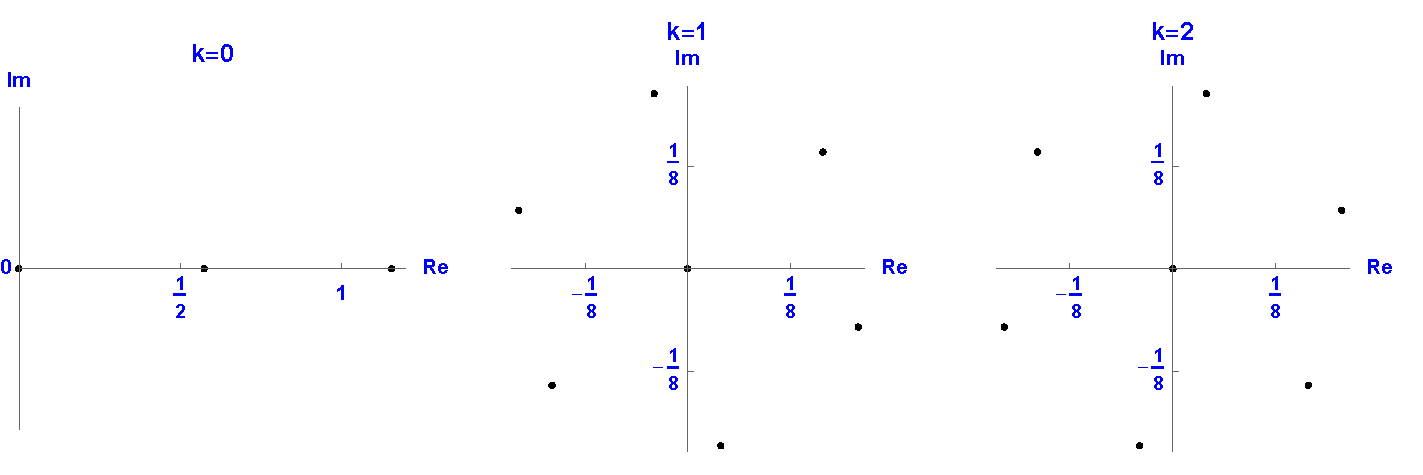
\includegraphics[width=\textwidth]{HLBernoulliC3}
  \caption{\label{fig:HLBernoulliC3}
Period-3 {\lattstate}s of the {temporal Bernoulli} with $s=2$, plotted in the $\Cn{3}$
permutation irreps subspaces.
}
\end{figure}
%%%%%%%%%%%%%%%%%%%%%%%%%%%%%%%%%%%%%%%%%%%%%%%%%%%

%%%%%%%%%%%%%%%%%%%%%%%%%%%%%%%%%%%%%%%%%%%%%%%%%%%%%%%%%%%%%
\begin{figure}\begin{center}
            \begin{minipage}[c]{0.45\textwidth}\begin{center}
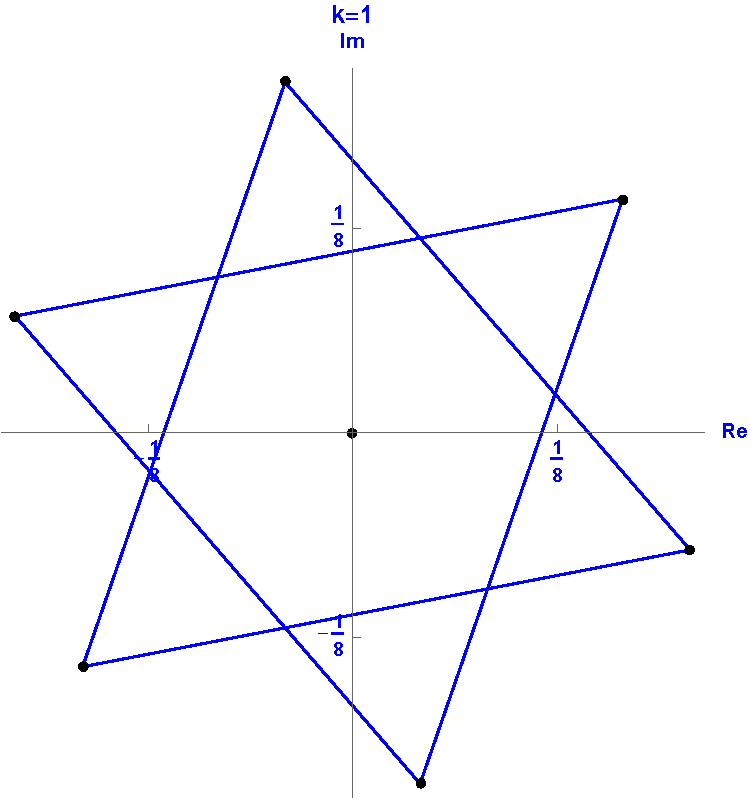
\includegraphics[width=1.0\textwidth]{HLBernoulliC3Orbits}\\
            \end{center}\end{minipage}
\end{center}
  \caption{\label{fig:HLBernoulliC3InvariantOrbits}
Period-3 {\lattstate}s of the {temporal Bernoulli} with $s=2$ in the subspace of
$k=1$ irrep.
{\Lattstate}s that are related by cyclic permutations are connected by blue lines.
The two triangles are 2 \Cn{3} orbits. The state in
the center is the fixed point.
}
\end{figure}
%%%%%%%%%%%%%%%%%%%%%%%%%%%%%%%%%%%%%%%%%%%%%%%%%%%%%%%%%%%%%%%

\subsubsection{Dihedral group}
\label{sect:LC21irrepsDn}

In the $\cl{}$\dmn\ space of the period-$\cl{}$ {\lattstate}s, the permutation representation
of the Dihedral group \Dn{\cl{}} can be generated by the shift operator matrix representation
\refeq{hopMatrix} and the reflection operator matrix representation:
\bea
\Refl=
\left(
\begin{array}{ccccc}
 1 &&&&0\\
  &  &  & 0 & 1 \\
  &  & \reflectbox{$\ddots$} & 1 &  \\
  & 0 & \reflectbox{$\ddots$} &  &  \\
  0& 1 &  &  &  \\
\end{array}
\right) \,.
\eea

The Dihedral group $\Dn{\cl{}}$ has: 2 1\dmn\ irreps and $[(\cl{}-1)/2]$
2\dmn\ irreps if $\cl{}$ is odd,
or 4 1\dmn\ irreps and $(\cl{}/2-1)$ 2\dmn\ irreps if $\cl{}$ is even.
If $\cl{}$ is odd, the permutation representation can be block diagonalized into irreps:
$A_0 \oplus E_1 \oplus \dots \oplus E_{(\cl{}-1)/2}$.
If $\cl{}$ is even, the permutation representation can be block diagonalized into irreps:
$A_0 \oplus B_1 \oplus E_1 \oplus \dots \oplus E_{\cl{}/2-1}$.

%%%%%%%%%%%%%%%%%%%%%%%%%%%%%%%%%%%%%%%%%%%%%%%%%%%
\begin{figure}
  \centering
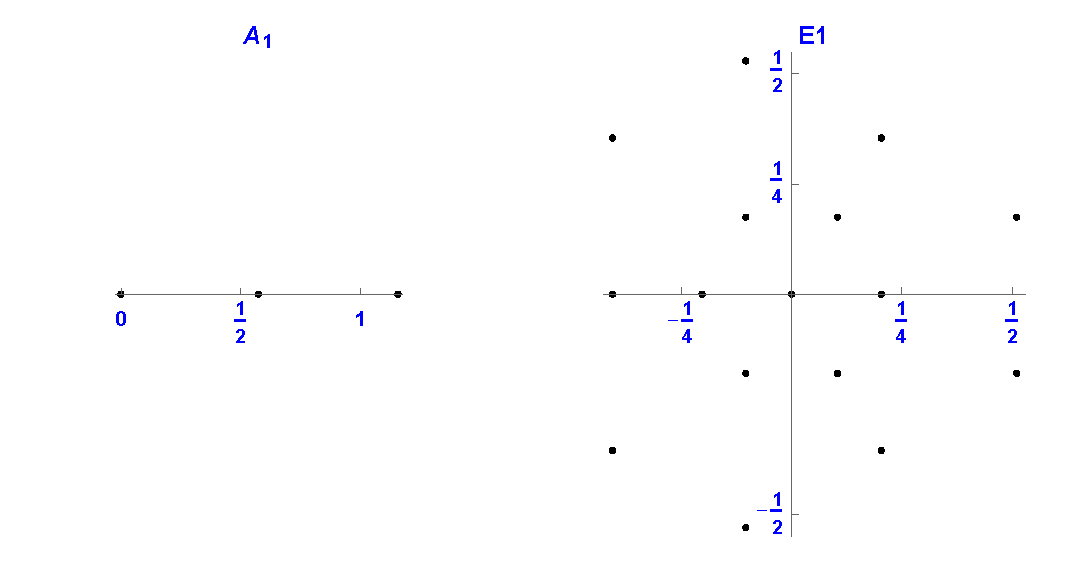
\includegraphics[width=0.8\textwidth]{HLCatmapD3}
  \caption{\label{fig:HLCatmapD3}
Period-3 {\lattstate}s of the $s=3$ \templatt, plotted in the $\Dn{3}$
permutation irreps subspaces $A_0+E$. In contrast with the
\Cn{\cl{}} complex irreps (see the \Cn{3} example
\reffig{fig:HLBernoulliC3}), the 2\dmn\ irrep $E\in\reals^2$ is real.
}
\end{figure}
%%%%%%%%%%%%%%%%%%%%%%%%%%%%%%%%%%%%%%%%%%%%%%%%%%%

%%%%%%%%%%%%%%%%%%%%%%%%%%%%%%%%%%%%%%%%%%%%%%%%%%%%%%%%%%%%%
\begin{figure}\begin{center}
            \begin{minipage}[c]{0.45\textwidth}\begin{center}
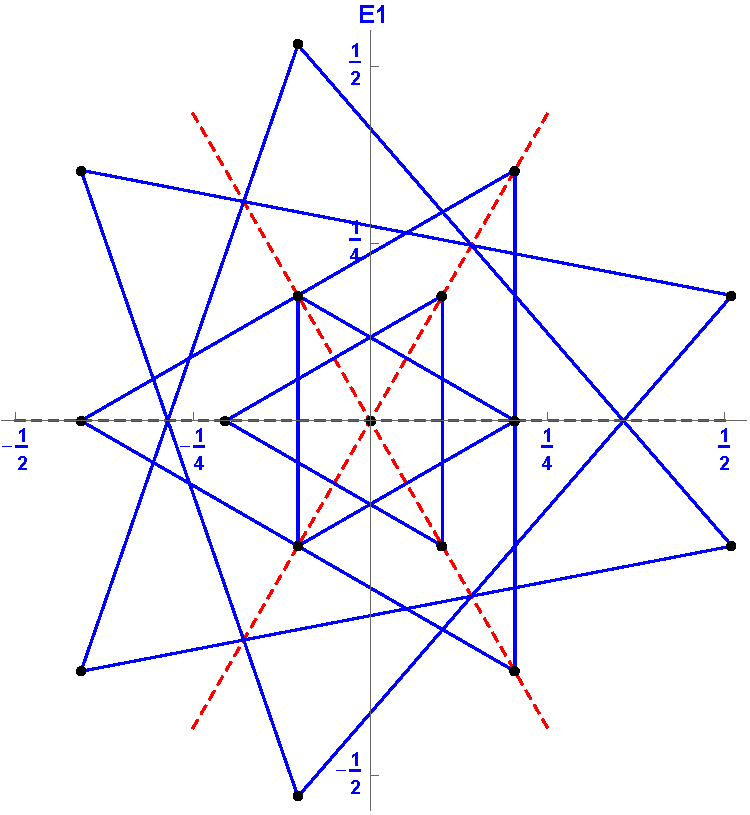
\includegraphics[width=1.0\textwidth]{HLCatmapD3Orbits}\\(a)
            \end{center}\end{minipage}
            \begin{minipage}[c]{0.45\textwidth}\begin{center}
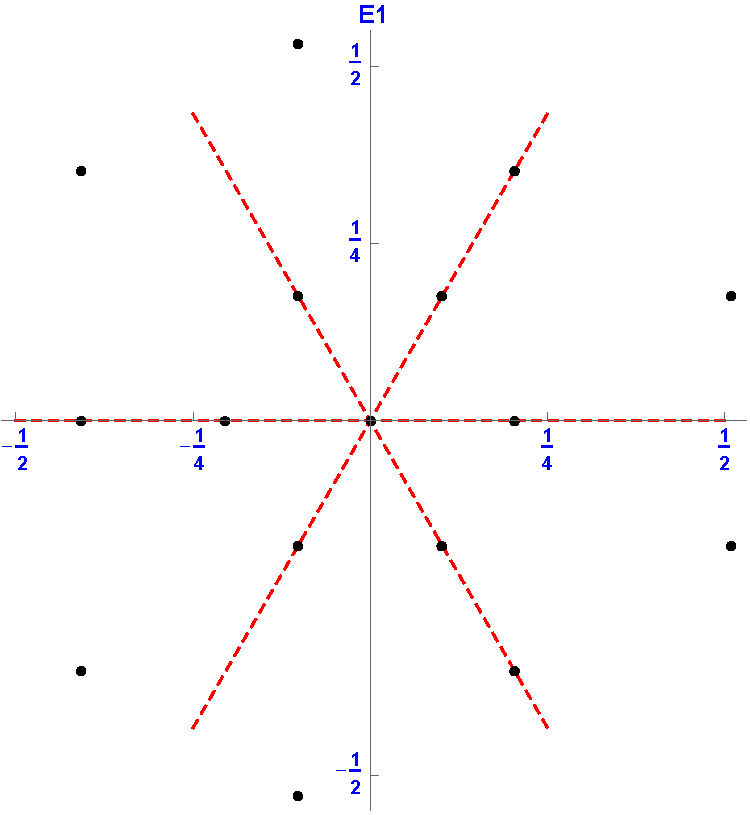
\includegraphics[width=1.0\textwidth]{HLCatmapD3InvariantStates}\\(b)
            \end{center}\end{minipage}
\end{center}
  \caption{\label{fig:HLCatmapD3InvariantOrbits}
Period-3 {\lattstate}s of the {\tempLatt} with $s=3$ in the subspace of
$E_1$ irrep.
(a):
{\Lattstate}s that are related by cyclic permutations are connected by blue lines.
The two big triangles are a single \Dn{3} 6-{\lattstate}s orbit, what for
\Cn{3} is a pair of 3-{\lattstate}s orbits without time reversal symmetry.
The remaining three smaller triangles are 3 time-reversal symmetric orbits;
the pair in the middle is presumably related by the
 $\Dn{1}: S\ssp_i = 1-\ssp_i$ invariance specific to
the \templatt, a symmetry not yet taken into account. The state in
the center is the fixed point.
(b):
Red dashed lines are the reflection axes of the $\Dn{3}$ group. There are 4 states
on each reflection axis.}
\end{figure}
%%%%%%%%%%%%%%%%%%%%%%%%%%%%%%%%%%%%%%%%%%%%%%%%%%%%%%%%%%%%%%%

When we use the similarity transformation to diagonalize the permutation representation,
the {\lattstate}s are transformed into the subspaces of the irreps.
The example of period-3 {\lattstate}s of \templatt\ with $s=3$ is shown in
\reffigs{fig:HLCatmapD3}{fig:HLCatmapD3InvariantOrbits}. The permutation
representation is block diagonalized by basis vectors: $e_0=1/\sqrt{3}(1,1,1)$,
$e_1=\sqrt{2/3}(\cos(2\pi/3),\cos(4\pi/3),1)$ and $e_2=\sqrt{2/3}(\sin(2\pi/3),\sin(4\pi/3),0)$.
The basis vector $e_0$ spans the subspace of the 1\dmn\ irrep $A_0$.
Basis vectors $e_1$ and $e_2$ span the subspace of the 2\dmn\ irrep $E$.

Period-3 {\lattstate}s of cat map with $s=3$ are mapped into the subspace
of the irreps $A_0$ and $E$ in \reffig{fig:HLCatmapD3}.
The irrep $A_0$ is the symmetric 1\dmn\ irrep, so in the subspace of $A_0$ the components
of {\lattstate}s are invariant under the action of the $\Dn{3}$ group.
In the 2\dmn\ subspace of the irrep $E$, the shift operator $\shift$ rotates the
{\lattstate}s clockwise by $2\pi/3$, while the reflection operator $\Refl$ reflects the {\lattstate}s
over the axis passing through the origin and pointing toward $(\cos(2\pi/3),\sin(2\pi/3))$.
In \reffig{fig:HLCatmapD3InvariantOrbits}
{\lattstate}s that are related by shifts are connected by blue lines.
The red dashed lines are reflection axis of the reflection operators.
The 2 big triangles in \reffig{fig:HLCatmapD3InvariantOrbits} (a) are lattice states
that belong to 2 orbits which are related by time reflection. The rest 3 triangles
are lattice states from 3 orbits which are invariant under time reflection.

\subsection{Fundamental domain} % of the {\lattstate}}

Given the space of the field configuration and the symmetry group acting on it,
we can find a fundamental domain such that each orbit in this space
visits the fundamental domain only once.
Each {\lattstate} in the fundamental domain is a representative {\lattstate} of an
orbit.
    \PC{2021-10-12}{
    Please read our draft\rf{LC21}, and either follow
    our definition \refeq{1dLattStat} of {\em {\lattstate}},
    or replace it with some other definition.
    }

One method to find the fundamental domain is based on the decomposition
of the space into the subspaces of the irreps of the symmetry group.
A natural way to choose the fundamental domain is to divide in the
subspace of an irrep, where the irrep divides the subspace into the number
of copies that is equal to the order of the symmetry group.

For example, in the space of the field configuration with \Cn{\cl{}} symmetry, the $k=1$ subspace
spanned by the eigenstate $\tilde{e}_1$, defined in \refeq{FourierModes}, can be divided
into $\cl{}$ copies. One can choose the region in the complex plane of $k=1$ subspace
with argument $0\leq\arg(\cssp_{1})<2\pi/\cl{}$ to be the fundamental domain.
Each orbit can visit the fundamental domain only once. As shown in \reffig{fig:HLBernoulliC3InvariantOrbits},
there are 3 points in this region, which are representative {\lattstate}s of two different
period-3 orbits and the fixed point $0$.

If the space of the field configuration has \Dn{\cl{}} symmetry,
the subspace of the 2\dmn\ irrep $E_1$ can be divided
into $2\cl{}$ copies by the irrep. One can choose the fundamental domain to be the region
with polar angle between 0 and $\pi/\cl{}$, assuming that the horizontal axis is one of the
reflection axis of the irrep $E_1$. Each orbit only appears once in the fundamental domain,
as shown in \reffig{fig:HLCatmapD3InvariantOrbits}. Note that the two orbits related by
the time reflection are considered one orbit of the dihedral group.

What happens when {\lattstate}s appear on the boundary of the fundamental domain?
There are two possible situations. The first situation is that the {\lattstate} belongs to an
orbit with multiplicity less than the order of the symmetry group. For example,
in \reffig{fig:HLCatmapD3InvariantOrbits}, there are 3 points in the fundamental domain
with polar angle equal to 0 or $\pi/3$. These 3 points are representative {\lattstate}s of orbits
with time reflection symmetry. The multiplicities of these orbits are 3 instead of 6.

The second situation is that the multiplicity of
the orbit of the {\lattstate} is equal to the order of the symmetry group
but the component in the subspace is 0. For example,
\[
\Xx = \frac{1}{104} (17, 51, 49, 43, 25, 75)
\]
is a period-6 {\lattstate} of the temporal Bernoulli
\refeq{LC21:1dBernLatt} with $s=3$. Using the discrete Fourier transform
this {\lattstate} becomes:
\[
\cssp =
\left(\frac{5}{2 \sqrt{6}},0,\frac{-5-3 i \sqrt{3}}{13
   \sqrt{6}},-\frac{\sqrt{3}}{4\sqrt{2}},\frac{-5+3 i \sqrt{3}}{13 \sqrt{6}},0\right) \,.
\]
This is a period-6 {\lattstate}. It belongs to an orbit that
contains 6 different {\lattstate}s. The $k=1$ component of this lattice
state is 0, which is on the boundary of the fundamental domain. To put this kind of
{\lattstate}s into the fundamental domain one needs to divide other subspaces.
For this lattice state the $k=2$ and $k=3$ components are not 0. The irreps divide
the $k=2$ subspace into 3 copies and the $k=3$ subspace into 2 copies. One way to
choose the fundamental domain in these subspaces is: the argument of the component
in the $k=1$ subspace is $0\leq\arg(\cssp_{1})<\pi/3$; if the $k=1$ component
is 0, the arguments of the components
in the $k=2$ and $k=3$ subspaces are $0\leq\arg(\cssp_{2})<2\pi/3{}$ and
$0\leq\arg(\cssp_{3})<\pi$. Each orbit is guaranteed to visit this fundamental
domain exactly once.

\bigskip
------------------------------------

If, in addition, the law is time-reversal (or time-inversion) invariant,
the symmetry includes time-reflection, ie, it is dihedral group \Dn{n}
with 2$\cl{}$ elements, so the reciprocal lattice should be a half of the
above 1/$\cl{}$ sliver of a $\cl{}$-gon, and irreps are now either 1 or 2
dimensional. Even $\cl{}$ is different from odd $\cl{}$, and solutions either appear
in pairs, or are self dual under reflection in 3 different ways.

Due to the time
reversal, all $k={2\pi}/{5}$ irrep states are the same as the
$k={4\pi}/{5}$ irrep states.

\newpage % REMOVE
    \input{../spatiotemp/chapter/LC21JacobianOrb}
\newpage % REMOVE
    % siminos/reversal/Hill.tex      pdflatex LC21; bibtex LC21
% temporary: siminos/spatiotemp/chapter/LC21Hill.tex
% $Author: predrag $ $Date: 2021-12-24 01:25:20 -0500 (Fri, 24 Dec 2021) $

%\renewcommand{\Ssym}[1]{{\ensuremath{m_{#1}}}}
\renewcommand{\statesp}{state space}
\renewcommand{\Statesp}{State space}
\renewcommand{\stateDsp}{state-space}
\renewcommand{\StateDsp}{State-space}

\section{% Hill's formula:
         Stability of an orbit vs. its time-evolution stability}
\label{s:LC21Hill}
% PC started with: siminos/kittens/Hill.tex  2021-08-19

In 1878-1886 a study of stability of the planar motion of the moon around
the earth led  Hill to the \emph{Hill's formula}\rf{Hill86}
\beq
\left|\Det\jMorb_c \right|= \left|\det (\id - \jMat_c)\right|
%\,.
\ee{detDet}
which relates the characteristic polynomial of the for\-ward-in-time
evolution {\po} Floquet stability matrix (monodromy matrix) $\jMat_p$ to the
determinant of the global {\jacobianOrb} $\jMorb_p$ (in Lagrangian settings,
the Hessian, the second variation of the action functional).
The discrete-time Lagrangian systems' Hill's formula
% \refeq{MacMei83(17)}
that we use here was derived by Mackay and Meiss\rf{MacMei83} in 1983.

Hill was lucky: he computed $\Det\jMorb_c$ in a $3\times 3$ Fourier modes
matrix approximation, which turned out to be quite a good approximation.
But this is a remarkable formula, especially in the limit of
$\cl{}\to\infty$ infinitesimal time steps, that relates a
field-theoretic, $\infty$\dmn\ \emph{functional} {\HillDet}
$\Det\jMorb_c$ to a determinant of the finite, $[d\times{d}]$ matrix
$\jMat_c$, and it took \Poincare\rf{Poinc1886} to prove that Hill's
Fourier modes calculation is correct in the continuum limit.

the {\jacobianOrb}  and the temporal evolution
\refeq{PV2config} stability ${{\hat{\mathbf{\jMat}}_{p}}}$ are related by
the remarkable (discrete time) Hill's formula\rf{MacMei83,BolTre10}
which expresses the  {\HillDet} of the arbitrarily large \jacobianOrb\
$\jMorb$  in terms of a determinant of a small
[$2\speriod{}\!\times\!2\speriod{}$] time-evolution \jacobianM\
$\hat{\mathbf{\jMat}}_p$.


While first discovered in a Lagrangian setting, Hill's formulas are much
more general, with the Lagrangian formalism of
\refrefs{MacMei83,TreZub09,BolTre10,kooknewt} --just a special case-- only
getting in way of understanding them.
As the formula is fundamental to the formulation
of the \spt\ chaotic field theory, we shall
rederive it here in several ways, relying on nothing more than elementary
linear algebra, in order to emphasize that formula applies to dissipative dynamical
systems as well, from the Bernoulli map to \NS\ and
\KS\rf{GudorfThesis,GuBuCv17}.


\bigskip

Assume that a \po\ $\ssp(\period{p}+\zeit)=\ssp(\zeit)$ of a continuous
time flow
\(
\dot{\ssp}=\vel(\ssp)
\)
is known `numerically exactly', that is to say, to arbitrary (but not
infinite) precision. One way to present the solution is to give a single
point $\ssp(0)$ in the orbit, and let the reader reconstruct the orbit
$p$ by integrating forward in time,
$\ssp(\zeit)=\hat{\map}^\zeit(\ssp(0))$, $\zeit\in[0,\period{p}]$.

However, for a linearly unstable \po\ a single point does not suffice to
present the orbit, because there is always a finite `Lyapunov time'
$\zeit_{Lyap}$  beyond which $\hat{\map}^\zeit(\ssp(0))$ has lost all memory of
the \po\ $p$. This problem is particularly severe in searches for {`\ecs
s'} embedded in turbulence, where even the shortest period solutions have
to be computed to the (for everyday fluid dynamics excessive) machine
precision\rf{GHCW07,channelflow,openpipeflow} in order to complete the
first return to the initial state.

Instead of relaying on for\-ward-in-time numerical integration,
\emph{global methods} for finding periodic orbits\rf{ChoGuck99} view them
as equations for the vector fields $\dot{\ssp}$ on spaces of closed
curves. In numerical implementations one discretizes the \po\  $p$ into
sufficiently many short
segments\rf{auto,GM00aut,ChoGuck99,DingCvit14,DCTSCD14}, and lists a
point for each segment
\beq
p=(\ssp_1,\ssp_2,\cdots,\ssp_\cl{p})
\,.
\ee{nXdCycle}
For a $k$\dmn\ discrete time map $\hat{\map}$ obtained by cutting the flow by a
set of {\PoincSec s}, with the \po\ $p$ of discrete period $\cl{p}$,
every segment can be reconstructed by a short time integration, and
satisfies
\beq
\ssp_{k+1}=\hat{\map}(\ssp_k)
\,,
\ee{CyclePntErr}
to high accuracy, as for sufficiently short times the exponential
instabilities are numerically controllable.


\bigskip

The temporal Bernoulli {\jacobianOrb} %\refeq{1stepVecEq},
$\jMorb=\partial/\partial\zeit-(s-1)\,\shift^{-1}$ is a differential
operator whose determinant one usually computes by a Fourier transform
diagonalization (see \refsect{sect:LC21recip1d}). The Fourier discretization
approach goes all the way back to Hill's 1886 paper\rf{Hill86};


\bigskip

In preparing this summary we have found expositions of Lagrangian
dynamics for discrete time systems by MacKay, Meiss and
Percival\rf{MKMP84,meiss92}, and Li and Tomsovic\rf{LiTom17b} particulary
helpful.

This formula was derived by Mackay and Meiss\rf{MacMei83} and
Allroth\rf{Allroth83} (Allroth eq.~(12)). It applies to general
``one-degree-of-freedom'' systems, \ie, 1D lattices with only the nearest
neighbor interactions. For a finite set of neighbors, \ie, higher\dmn\
discrete-time systems, Allroth\rf{Allroth83} has some partial results in the
context of Frenkel-Kontorova models.

{\HillDet}\rf{MacMei83,BolTre10,Verdiere07};
discrete Hill's formula and the Hill discriminant, Toda lattice\rf{Toda89}.

Toda\rf{Toda89} % {\em Theory of Nonlinear Lattices},
Chapt.~4.{\em Periodic Systems}

Toda studies the classical mechanics of one-dimensional
lattices (chains) of particles with nearest neighbor interaction; they
are discrete and infinite in space, continuous in time.

The {\em inverse scattering method} for an infinite lattice makes use of
the discrete Schrodinger equation. For periodic systems this gives a
discrete Hill's equation, and in place of the scattering data, it is
convenient to use the spectrum of the discrete Hill's equation.
 Thus the initial value problem reduces to the inverse problem
(Jacobi's inverse problem), or inverse spectral theory.

Toda discrete Hill's equation is continuous in time, so presumably the most
of the work is for stationary states.

He works with a 3-term recurrence (4.1.3a), and defines a 2-configuration
monodromy matrix (4.1.11).

For special values of A, the solution of (4.1.4) can be periodic, but
more generally it is relative periodic (4.1.16), or the Bloch function
(it's existence given by the Floquet theorem).
His \jacobianOrb\ (4.1.28) has variable diagonal and off
diagonal elements, corresponding to nontrivial nonlinear solutions for
$d=1$ lattice.

Historically,  in \po\ theory
calculations one always computes $\jMat_\Mm$. However, as we shall show
here, and in more generality in \refsect{s:Hill}, it is the {\HillDet}
$\Det\jMorb$ that is the computationally robust quantity that one should
evaluate.

\begin{quote}
A succinct  explanation of the Hill's formula:\\
If you evaluate stability of the 3-term recurrence \refeq{JiKoKr20(2)} on
a periodic lattice you get the {\jacobianOrb} $\jMorb$;
if you evaluate it by multiplying the `two-configuration representation'
matrix $\jMps$, you get the `time evolution' side of the Hill's formula.
\end{quote}


% PC 2021-10-23
%     moved from siminos/spatiotemp/chapter/LC21Bernoulli.tex
\subsection{{\HillDet} for a $d$-component lattice field}
\label{s:LC21notHill}   % was {exam:Hill1stOrd}
% maybe call this {Hill's formula for a general first-order system}
% siminos/spatiotemp/Examples/examHill1stOrd.tex

The {\jacobianOrb} $\jMorb_{\zeit\zeit'}$ \refeq{jacobianOrb} is a
high-\dmn\ linear stability matrix for the extremum condition
$F[\Xx_c]=0$, evaluated on the {\lattstate} $\Xx_c$. How is the stability
so computed related to the conventional dynamical systems'
for\-ward-in-time stability? To motivate the answer in its generality,
consider a temporal lattice with a set of $d$ fields
$\ssp_{\zeit}=\{\ssp_{\zeit,1},\ssp_{\zeit,2},\dots,\ssp_{\zeit,d}\}$ on
each lattice site $\zeit$, and time evolution given by a $d$\dmn\ map
$\ssp_{\zeit+1}=\hat{\map}(\ssp_{\zeit})$.
A period-$\cl{}$ {\lattstate} \refeq{pathBern} thus
satisfies site-by-site the first-order difference equation
\beq
\ssp_{\zeit} - \hat{\map}(\ssp_{\zeit-1}) = 0
    \,,\qquad
\zeit=1,2,\cdots,\cl{}
\,.
\ee{1stepNonlimTemp}
A small deviation $\Delta\Xx$ from $\Xx_p$ then satisfies the linearized condition
\beq
\Delta\ssp_{\zeit} - \shift^{-1}\jMat_{\zeit}\,\Delta\ssp_{\zeit} = 0
\,,\qquad
(\jMat_{\zeit})_{ij}
=
        %\left.
        \frac{\partial \flow{}{\ssp_\zeit}_i }
             {\partial \ssp_j                }
        %\right|_{\ssp_{j}=\ssp_{\zeit,j}}
\,,
\ee{d-1stepJac2}
where $\jMat_{\zeit}$ is the 1-time step $[d\!\times\!{d}]$
\jacobianM, evaluated on lattice site $\zeit$.

It suffices to work out a temporal period $\cl{}=3$ example to understand
the calculation for any period. In terms of the $[3d\!\times\!3d]$
generalized \refeq{hopMatrix} block shift matrix $\shift$, the \jacobianOrb\
\refeq{jacobianOrb} has block matrix form
\beq
\jMorb_p \,=\,
\id-\shift^{-1}\jMat
\,,\quad
\shift =
\left[
\begin{array}{ccc}
0     & \id_d& 0   \\
0     & 0     & \id_d\\
\id_d& 0     & 0
\end{array}
\right]
\,,\quad
\jMat =
\left[
\begin{array}{ccc}
\jMat_1 & 0 & 0 \\
0 & \jMat_2 & 0  \\
0 & 0 & \jMat_3
\end{array}
\right]
\,,
\ee{3shift}
where $\id  $ is the $d$\dmn\ identity matrix.
Next, consider
\beq
\shift^{-1}\jMat =
\left[
\begin{array}{ccc}
0       & 0       & \jMat_3   \\
\jMat_1 & 0       & 0  \\
0       & \jMat_2 & 0
\end{array}
\right]
,\;\;
(\shift^{-1}\jMat)^2 \,=\,
\left[
\begin{array}{ccc}
0 & \jMat_3\jMat_2 & 0 \\
0 & 0 & \jMat_1\jMat_3  \\
\jMat_2\jMat_1 & 0 & 0
\end{array}
\right]
\,,
\ee{stabShift}
and note that the $\cl{}=3$ repeat of $\shift^{-1}\jMat$ is block-diagonal
\bea
(\shift^{-1}\jMat)^3  =
\left[
\begin{array}{ccc}
\jMat_3\jMat_2\jMat_1 & 0 & 0 \\
0 & \jMat_1\jMat_3\jMat_2 & 0  \\
0 & 0 & \jMat_2\jMat_1\jMat_3
\end{array}
\right]
\,,
\label{stabCube}
\eea
with $[d\!\times\!{d}]$ blocks cyclic permutations of each other.f
In general, % as $\shift^\cl{}=\id$,
the trace of the
$[\cl{}d\!\times\!\cl{}d]$ matrix for a period $\cl{}$ {\lattstate}
\[
\Tr(\shift^{-1}\jMat)^k=\delta_{k,r\cl{}}\,\cl{}\,\tr\jMat_p^r
\,,\quad
\jMat_p = \jMat_\cl{}\jMat_{\cl{}-1}\cdots\jMat_2\jMat_1
\]
is non-vanishing only if $k$ is a multiple of $\cl{}$, where $\jMat_p$ is the
for\-ward-in-time $[d\!\times\!{d}]$ Floquet matrix of the \po\ $p$.

Now we can evaluate the {\HillDet}
$\Det\jMorb_p$ by expanding
\bea
\ln\Det\jMorb_p &=&
\Tr\ln(\id-{\shift}^{-1}\jMat)
                \,=\,
-\sum_{k=1}^\infty\frac{1}{k}\,\Tr({\shift}^{-1}\jMat)^k
    \continue
                 &=&
-\tr\sum_{r=1}^\infty\frac{1}{r} \jMat_p^{r}
  =
\ln\det(\id_d-\jMat_p)
\,.
\label{LnDet=TrLn2}
\eea
The {\jacobianOrb} $\jMorb_p$ evaluated on a {\lattstate} $\Xx_p$
satisfying the temporal lattice first-order difference equation
\refeq{1stepNonlimTemp}, and the dynamical, for\-ward-in-time \jacobianM\
$\jMat_p$ are thus related by \emph{Hill's formula}
\beq
\Det\jMorb_p = \det(\id  -\jMat_p)
\,,
\ee{detDet}
which relates the global orbit stability to the Floquet, for\-ward-in-time
evolution stability.

As far as the time-evolution stability is concerned, the
$|\Det\jMorb_\Mm|=|\det (\id-\jMat_\Mm)|$ formula \refeq{detDet} is
correct for all first-order difference equations (systems whose evolution
laws are first order in time), for any $[d\times{d}]$ one-time-step
{\jacobianM}. For the Bernoulli system that is a $[1\!\times\!1]$ matrix
$\jMat=s$, with the periodic points count \refeq{detBern2} trivially
verified.

The temporal {Bernoulli} \refeq{tempBern} is a particularly simple, linear  example.
The site field $\ssp_\zeit$ is a scalar,
the 1-time step $[1\!\times\!1]$ time-evolution \jacobianM\
\refeq{d-1stepJac2} at every lattice point $\zeit$ is simply
$\jMat_{\zeit}={s}$,
and
the {\jacobianOrb}
\refeq{tempBern} is the same for all {\lattstate}s of period $\cl{}$,
so
\beq
\mbox{temporal {Bernoulli}: }\quad
N_\cl{} = |\Det\jMorb| = {s}^{\cl{}} - 1
\,,
\ee{LC21detBern}
in agreement with the time-evolution count \refeq{noPerPtsBm}; all
itineraries are allowed, except that the periodicity of
$\shift^\cl{}=\id$ accounts for $\cycle{0}$ and
$\cycle{s\!-\!1}$ fixed points (see \reffig{fig:BernPart}) being a
single periodic point.



\subsection{{\HillDet} of a for\-ward-in-time map}
\label{s:LC21forwardHill}

For a $d$\dmn\ deterministic map $\ssp_{\zeit+1} = \hat{\map}(\ssp_{\zeit})$, the
{\FPoper}
\beq
     \Lop\,\msr(\ssp_{\zeit+1})
= \int_\pS\!\! d\ssp_{\zeit}\,
           \delta(\ssp_{\zeit+1} - \hat{\map}(\ssp_{\zeit}))\,
           \msr(\ssp_{\zeit})
%\,,
\ee{PerronFrobenius}
maps a density distribution $\msr(\ssp_{\zeit})$ for\-ward-in-time.
Its kernel, a $d$\dmn\ Dirac delta function
\bea
\Lop(\ssp_{\zeit+1},\ssp_{\zeit})
    = \delta(\ssp_{\zeit+1} - \hat{\map}(\ssp_{\zeit}))
\,,
\eea
applied repeatedly satisfies the group property
\beq
\Lop^2(\ssp_{\zeit+2},\ssp_{\zeit})
    = \int_\pS\!\! d\ssp_{\zeit+1}\,
            \Lop(\ssp_{\zeit+2},\ssp_{\zeit+1})\,
            \Lop(\ssp_{\zeit+1},\ssp_{\zeit})
    = \delta(\ssp_{\zeit+2}-\flow{2}{\ssp_{\zeit}})
\,.
\ee{FPsemiGroup}
The time-evolution periodic orbit theory\rf{ChaosBook} relates the
long time chaotic averages to the traces of the {\FPoper}
\beq
\tr\Lop^\cl{}
     = \int_\pS\!\!d\ssp\,\Lop^\cl{}(\ssp,\ssp)
     = \int_\pS\!\!d\ssp_{c}\,\delta(\ssp_{c} - \flow{\cl{}}{\ssp_c})
\eeq
and its weighted, evolution operator generalizations, with support on all
periodic points / {\lattstate}s   $\ssp_{c}=\flow{\cl{}}{\ssp_c}$ of
period $cl{}$.

To evaluate the trace of the $\cl{}$th iterate of the {\FPoper},
one can either use the kernel of the operator
$\Lop^\cl{}(\ssp_{\cl{}},\ssp_0) = \delta(\ssp_{\cl{}} - \flow{\cl{}}{\ssp_0})$,
\bea
\tr \Lop^\cl{} &=&  \int_\pS\!\!d\ssp_0 \, \delta(\ssp_{0}-\flow{\cl{}}{\ssp_0})
\,,
\eea
or, using the group property \refeq{FPsemiGroup} to insert integrations
over intermediate lattice sites, the product of one-time-step operators $\Lop$:
\bea
\tr \Lop^\cl{} &=&
\int  d\Xx \prod_{\zeit=0}^{\cl{}-1} \delta(\ssp_{\zeit+1}-\hat{\map}(\ssp_{\zeit})) \,,
\continue
\ssp_{\cl{}} &=& \ssp_0 \,, \quad d\Xx
              = \prod_{\zeit=0}^{\cl{}-1} d \ssp_{\zeit}
\,.
\label{PerronFrobeniusTrace}
\eea
The field $\ssp_{\zeit}$ on every lattice site $\zeit$ is a $d$\dmn\
vector, so a period-\cl{} {\lattstate} \Xx\ is a $\cl{}d$\dmn\ vector,
with the Dirac function also $\cl{}d$\dmn. In matrix notation this trace
takes a compact form:
\bea
\tr \Lop^\cl{} = \int d\Xx\,\delta(\shift \Xx - \hat{\map}(\Xx)) \,,
\eea
where $\Xx$ and $\hat{\map}(\Xx)$ are $\cl{}d$\dmn\ column vectors with
$(id+j)$th components $(\ssp_{\zeit})_j$ and
$[\hat{\map}(\ssp_{\zeit})]_j$, where $0 \leq i < \cl{}-1$, $0 \leq j < d-1$,
and $\shift$ is the cyclic $[\cl{}d\!\times\!\cl{}d]$ {\shiftOp}
(compare with \refeq{hopMatrix}):
\beq
\shift
=  \left(\begin{array}{ccccc}
             0    &  \id      &        &   &  \cr
                  &  0    &   \id      &   &  \cr
                  &       &        & \ddots &  \cr
                  &       &        & 0 & \id   \cr
             \id      &       &        &   & 0
          \end{array} \right)
\,,
\eeq
where $\id  $ is the $d$\dmn\ identity matrix.
Note that the vector
in the $\cl{}d$\dmn\ Dirac delta function is the defining equation
\refeq{LC21eqMotion} of the system:
\[
F[\Xx] = \shift \Xx - \hat{\map}(\Xx) \,.
\]

\refeq{LC21eqMotion}
with a global deterministic solution $\Xx_c$ satisfying this local extremal
condition on every lattice site.


Restricting the integration to an infinitesimal neighborhood
$\pS_p$ around a periodic point $\ssp_p$, the contribution from this periodic point is:
\bea
\tr\left.\Lop^\cl{}\right|_p =
       \int_{\pS_p} \!\!d\ssp_0\,\delta(\ssp_{0}-\flow{\cl{}}{\ssp_0})
       =\frac{1}{\left|\det(\id - \jMat_p)\right|} \,,
\label{ForwardInTimeTr}
\eea
where $\jMat_p$ is the $[d\!\times\!d]$ for\-ward-in-time Floquet matrix of
the periodic orbit \refeq{d-1stepJac2} started from the periodic point
$\ssp_p$ with period $\cl{}$. Compute the trace using the integral on
$\cl{}$ points:
\bea
\tr_p \Lop^\cl{} &=&
\int_{\pS_p}\!\!d\Xx\,\prod_{i=0}^{\cl{}-1}
            \delta(\ssp_{\zeit+1}-\hat{\map}(\ssp_{\zeit}))
                  = \int_{\pS_{p}}\!\!\!d\Xx\,\delta(F[\Xx])
\continue
&=& \frac{1}{\left|\Det\jMorb_p\right|}
\,,
\label{GlobalTr}
\eea
where
\bea
\jMorb_p = \frac{\partial F[\Xx]}{\partial \Xx}
\eea
is the $[\cl{}d\!\times\!\cl{}d]$ {\jacobianOrb} of the period-$\cl{}$
{\lattstate} started with $\ssp_p$.
$\pS_{p}$ is a region in the $\cl{}d$\dmn\ \statesp\ of $\Xx$ whose first
$d$ components are the infinitesimal neighborhood around $\ssp_p$.
Comparing the trace \refeq{ForwardInTimeTr} and \refeq{GlobalTr}, we have
proved the Hill's formula \refeq{detDet}.

\subsection{{\HillDet} for a 2nd order difference equation}
\label{s:LC21Hill2step}

An $n$-step recurrence relation is the discrete-time analogue of an $n$th
order differential equation. In formulating dynamical systems problems,
one almost always replaces higher order derivatives (Euler-Lagrange
equations) by sets of fields satisfying first order equations (Hamilton's
equations), and the same is true for discrete time systems. For example,
the Hamiltonian \templatt\ and \HenonMap\ are usually formulated as
time-evolution over a 2\dmn\ phase space \refeq{catMap} and
\refeq{LC21eq2.1}, rather than the 3-term recurrence configuration space
conditions \refeq{catMapNewt} and \refeq{LC21:2-step}.

A $k$th order differential equation can be discretized as a $k$th order
difference equation. Just as a scalar field satisfying a $k$th order
differential equation can be replaced by a set of $k$ fields, each
satisfying a first order equation, a $k$th order difference equation for
a scalar field can be replaced by a $k$\dmn\ vector field, satisfying $k$
$1$st order difference equations.

One can compute the orbit stability of a scalar field {\lattstate} of
such system using the for\-ward-in-time Hill's formula for the $k$\dmn\
vector field representation of dynamics, and the corresponding the
determinant of the $[k\cl{} \times k\cl{}]$ {\jacobianOrb}
\refeq{GlobalTr}. However, with the recurrence relation, the
{\jacobianOrb} has a simpler form.

Consider a map with a 3-term recurrence relation, $\ssp_{\zeit+1} = \map(\ssp_{\zeit-1}, \ssp_{\zeit})$,
where $\ssp_{\zeit-1}$, $\ssp_{\zeit}$ and $\ssp_{\zeit+1}$ are scalars.
This map can be replaced by a pair of 1st order difference equations
$(\ssp_{\zeit}, \ssp_{\zeit+1}) = \hat{f}(\ssp_{\zeit-1}, \ssp_{\zeit}) = (\ssp_{\zeit}, \map(\ssp_{\zeit-1},\ssp_{\zeit}))$.
The trace of the $\cl{}$th iterate of the {\FPoper} can be
evaluated using the Dirac delta kernel of the operator $\Lop^\cl{}$, or the
product of $\Lop$ and the recurrence relation:
\bea
\tr \Lop^\cl{} &=&  \int d \ssp_0 d \ssp_1 \delta((\ssp_{0},\ssp_1) -
\hat{f}^\cl{}(\ssp_0,\ssp_1))
\continue
               &=&
\int [d \Xx] \prod_{i=0}^{\cl{}-1} \delta(\ssp_{\zeit+1}-\map(\ssp_{\zeit-1},\ssp_{\zeit})) \,,
\continue
\ssp_{\cl{}} &=& \ssp_0 \,, \quad
\ssp_{-1} = \ssp_{\cl{}-1} \,, \quad
[d \Xx] = \prod_{i=0}^{\cl{}-1} d \ssp_{\zeit} \,.
\eea
Using the matrix notation, the trace computed by
the integral on $\cl{}$ points along a discrete periodic orbit is:
\bea
\tr \Lop^\cl{} = \int [d \Xx] \delta(\shift \Xx - \map(\shift^{-1} \Xx, \Xx)) \,,
\eea
where $\Xx$ and $\map(\shift^{-1} \Xx, \Xx)$ are $\cl{}$\dmn\ column vectors with $i$th components
$\ssp_{\zeit}$ and $\map((\shift^{-1}\Xx)_i,\Xx_i)$, and $\shift$ is the cyclic $[\cl{}\!\times\! \cl{}]$
{\shiftOp} \refeq{hopMatrix}. The vector in the Dirac delta function is the defining equation of
the system:
\bea
F[\Xx] = \shift \Xx - \map(\shift^{-1} \Xx, \Xx) \,.
\eea
Restricting the integration to an infinitesimal neighborhood
$\pS_p$ around a periodic point $(\ssp_{p,0},\ssp_{p,1})$ with period $\cl{}$,
the contribution from this periodic point is:
\bea
\tr_p \Lop^\cl{} = \int_{\pS_p} d \ssp_0 d \ssp_1 \delta((\ssp_{0},\ssp_1) -
\hat{f}^\cl{}(\ssp_0,\ssp_1))
=\frac{1}{\left|\det(\id - \jMat_p)\right|} \,,
\label{ForwardInTimeTrRecurrence}
\eea
where
\bea
\jMat_p = \frac{\partial \hat{f}^{\cl{}}(\ssp_{p,0},\ssp_{p,1})}{\partial (\ssp_{p,0},\ssp_{p,1})}
\eea
is the $[2\!\times\!2]$ for\-ward-in-time Floquet matrix of the periodic orbit
started from the periodic point
$(\ssp_{p,0},\ssp_{p,1})$ with period $\cl{}$. Compute the trace using the
integral on $\cl{}$ points:
\bea
\tr_p \Lop^\cl{} &=&
\int_{\pS_{\Xx_p}} [d \Xx] \delta(\shift \Xx - \map(\shift^{-1} \Xx, \Xx))
                  = \int_{\pS_{\Xx_p}} [d \Xx] \delta(F[\Xx])
\continue
                 &=& \frac{1}{\left|\Det\jMorb_p\right|}
\,,
\label{GlobalTrRecurrence}
\eea
where
\bea
\jMorb_p = \frac{\partial F[\Xx_p]}{\partial \Xx_p}
\eea
is the $[\cl{}\!\times\!\cl{}]$
{\jacobianOrb} of the period-$\cl{}$ {\lattstate} started with $(\ssp_{p,0},\ssp_{p,1})$.
$\pS_{\Xx_p}$ is a region in the $\cl{}$\dmn\ space of $\Xx$ whose first 2
components are the infinitesimal neighborhood around $(\ssp_{p,0},\ssp_{p,1})$.
Compare the trace \refeq{ForwardInTimeTrRecurrence} and
\refeq{GlobalTrRecurrence}, we have proved the Hill's formula \refeq{detDet}.

\HL{2021-12-16}{The rest of this section is from the old version.
        }

Our task is to compute the {\HillDet} $|\det \jMorb|$. We first show how
to do that directly, by computing the volume of the {\fundPip}.

\subsection{{\HillDet}: fundamental parallelepiped evaluation}
\label{s:LC21fundFacteval}
% 2020-02-16 Predrag computed  using siminos/mathematica/Tensors.nb
As a concrete example
consider the Bravais lattice % \refeq{1DBravLatt}
with basis
vector

\subsection{{\HillDet}: time-evolution evaluation}
\label{s:LC21HillHam}

However, in classical and statistical mechanics, one often computes the
{\HillDet} using a  Hamiltonian, or `transfer matrix' formulation.

Define
\[  %\beq
\hat{\xx}_\zeit
=
\left[\begin{array}{l}
 {\ssp}_{\zeit-1}\\
 {\ssp}_\zeit
 \end{array}\right]
,\quad
\hat{\mathsf{\Ssym{}}}_\zeit
=
    \left[\begin{array}{l}
    {0}\\
 {\Ssym{}}_{\zeit}
 \end{array}\right]
\,,
\] %\ee{PV2catlattJ1}
where the hat $\hat{~}$~ indicates a $2$\dmn\
`two-configuration'\rf{PerViv} lattice site $\zeit$ state.

The $1$\dmn\ field theory 3-term recurrence \refeq{LC21:1dTempFT} written
in the \PV\rf{PerViv} `two-configuration representation'
\refeq{LC21PerViv}.


$\mathbf{\jMorb}_1$ is the spatial
$[\speriod{}\!\times\!\speriod{}]$ {\jacobianOrb} of
$d=1$ \templatt\ form \refeq{tempCatFix},


This proves that $\det\hat{\mathbf{\jMorb}}$ of the
`Hamiltonian' or `two-configuration'
$[2\speriod{}\cl{}\times2\speriod{}\cl{}]$ `phase space'
\jacobianOrb\ $\hat{\mathbf{\jMorb}}$ defined by \refeq{eq:orbitJPVJxS}
equals the `Lagrangian' {\HillDet} of the
$[\speriod{}\cl{}\times\speriod{}\cl{}]$ \jacobianOrb\
$\mathbf{\jMorb}$.


\subsection{{\HillDet}: Reciprocal lattice evaluation}

$\omega = e^{2i\pi/\cl{}}$

$\cssp_k=x_k+i\,y_k = |\cssp_k| e^{i\theta_k}$

$q_k=2\pi{k}/\cl{}$,

$\cl{}$ is the Bravais cell period

\bigskip

The temporal Bernoulli {\jacobianOrb} %\refeq{1stepVecEq},
$\jMorb=\partial/\partial\zeit-(s-1)\,\shift^{-1}$ is a differential
operator whose determinant one usually computes by a Fourier transform
diagonalization (see \refsect{sect:LC21recip1d}). The Fourier discretization
approach goes all the way back to Hill's 1886 paper\rf{Hill86}.

The first advantage of using the reciprocal lattice is that it provides a
way to compute the {\HillDet}.
If the \jacobianOrb\ \refeq{jacobianOrb} commutes with the translation
operator, the plane waves are eigenvectors of the \jacobianOrb. Using
these eigenvectors one can find the eigenvalues and the determinant of
the \jacobianOrb. In the $\cl{}$\dmn\ space of {\lattstate}s with
period-$\cl{}$, the one-lattice spacing translation operator is a shift
matrix \refeq{hopMatrix},
%\bea
%\shift
%=  \left(\begin{array}{ccccc}
%             0    &  1    &        &   &  \cr
%                  &  0    &   1    &   &  \cr
%                  &       &        & \ddots &  \cr
%                  &       &        & 0 & 1 \cr
%             1    &       &        &   & 0
%          \end{array} \right)
%\,,
%\eea
whose eigenvectors are plane waves $\tilde{e}_k$:
\bea
\shift\,\tilde{e}_k = \omega^{k} \tilde{e}_k \, .
\eea
For example, the eigenvalues of the {temporal Bernoulli}
{\jacobianOrb} \refeq{tempBern} are
% $(\id-{s}\,\shift^{-1})$ is given by:
% \jMorb =
\bea
({s}\id - {\shift})\,\tilde{e}_k
= ({s} - \omega^{k})\,\tilde{e}_k
\,,
\eea
and the {\HillDet} is simply a polynomial whose roots are the \cl{}th
roots of unity,
\bea
\Det({s}\id - {\shift})
=
\prod_{k=0}^{\cl{}-1} ({s} - \omega^{k})
=
s^{\cl{}} - 1
\,.
\eea
see \refeq{shift2n}.
The eigenvalues of the \templatt\
{\jacobianOrb} \refeq{tempCatFix} are:
\bea
(-\shift+{s}\,\id-\shift^{-1})\,\tilde{e}_k
=
({s} - 2\cos(2\pi k/\cl{}))\,\tilde{e}_k \, ,
\eea
and the {\HillDet} is:
\bea
\mbox{\templatt: }\quad
\Det(-\shift+{s}\,\id-\shift^{-1})
    &=&
\prod_{k=0}^{\cl{}-1} ({s} - 2\cos(2\pi k/\cl{}))
    \continue
    &=&
2 T_{\cl{}} \left({s}/{2}\right) - 2 \, ,
\eea
where $T_{\cl{}}$ is the Chebyshev polynomial of the first
kind.

%%%%%%%%%%%%%%%%%%%%%%%%%%%%%%%%%%%%%%%%%%%%%%%
\begin{figure}\begin{center}
            \begin{minipage}[c]{0.3\textwidth}\begin{center}
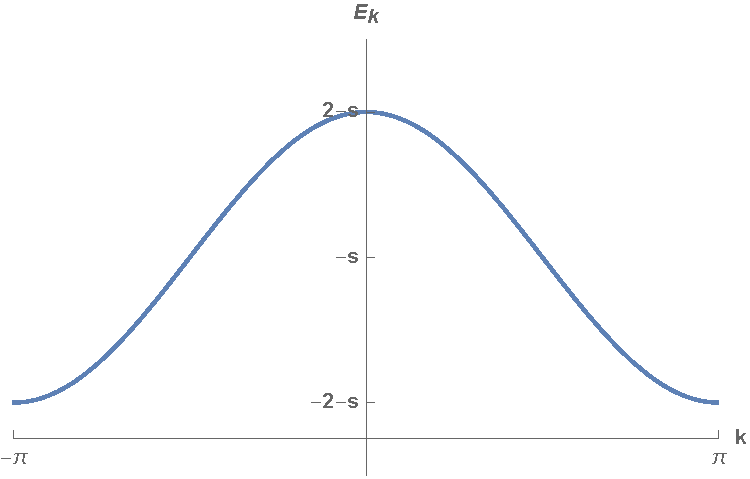
\includegraphics[width=1.0\textwidth]{HLTemplattBand}\\(a)
            \end{center}\end{minipage}
            \begin{minipage}[c]{0.3\textwidth}\begin{center}
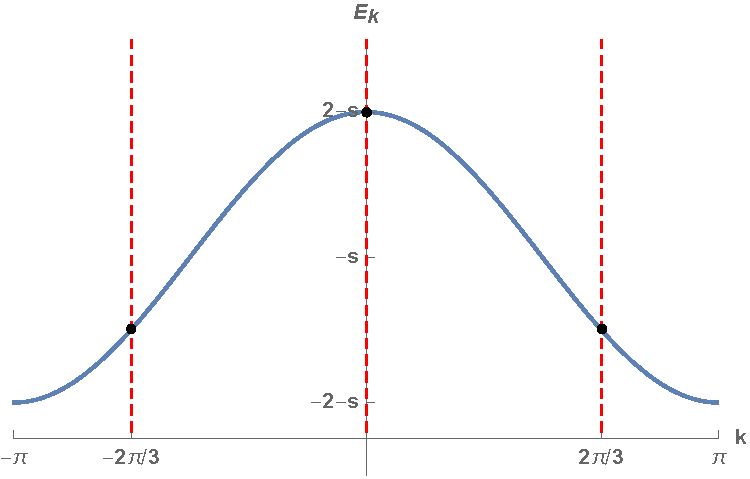
\includegraphics[width=1.0\textwidth]{HLTemplattBand3cycle}\\(b)
            \end{center}\end{minipage}
            \begin{minipage}[c]{0.3\textwidth}\begin{center}
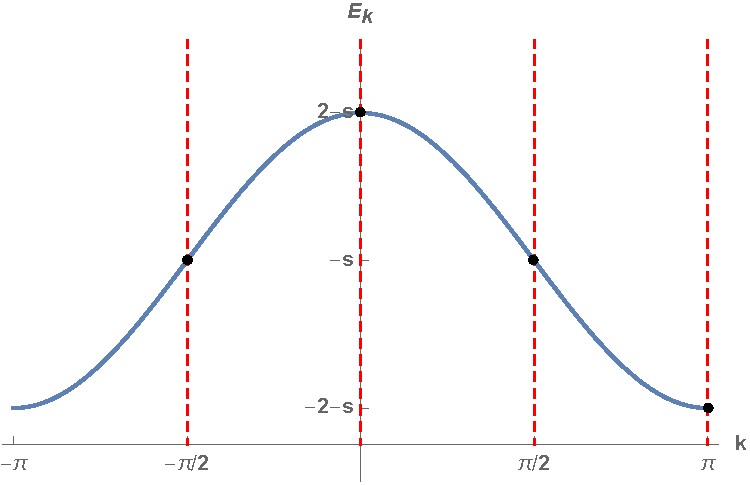
\includegraphics[width=1.0\textwidth]{HLTemplattBand4cycle}\\(c)
            \end{center}\end{minipage}
\end{center}
  \caption{\label{fig:LC21emplattBand}
(a) The eigenvalue $E_k$ of the \jacobianOrb\ on the infinite lattice as a function of the wave
vector $k$ in the first Brillouin zone. The \jacobianOrb\ has the reflection symmetry so the
eigenvalue is also invariant under the reflection $k\to -k$.
(b) For period 3 lattice states, the wave vectors of the eigenstates exist on the reciprocal lattice
spanned by $2\pi/3$. These lattice sites are labeled by the red dashed lines. There are only
3 period 3 eigenstates, with eigenvalues $-1-s$, $2-s$ and $-1-s$.
(c) For period 4 lattice states, the wave vectors of the eigenstates exist on the reciprocal lattice
spanned by $\pi/2$. These lattice sites are labeled by the red dashed lines. There are only
4 period 4 eigenstates, with eigenvalues $-s$, $2-s$, $-s$ and $-2-s$.
$k=\pi$ and $k=-\pi$ are different by a reciprocal lattice translation, so they are a same
wave vector and should be only counted once.
          }
\end{figure}
%%%%%%%%%%%%%%%%%%%%%%%%%%%%%%%%%%%%%%%%%%%%%%%

Explain \reffig{fig:LC21emplattBand}.

        \PC{2021-09-02} {
I think I prefer some version of the identity \refeq{TableOfISP13952},
\refeq{HillDetOrbJ},
no mention of Chebyshev polynomials. Not important, will revisit later.
    }


\subsection{Remarks}
\label{s:LC21HillForm}

Two remarks.
First, the reformulation of the \catlatt\ 3-term recurrence
% \refeq{CatMap2dHill}
as the `two-configuration' map \refeq{PV2config} is
a passage from the Lagrangian to the Hamiltonian formulation, also known
as `transfer matrix' formulation of lattice field
theories\rf{MonMun94,MunWal00} and Ising
models\rf{Onsager44,Kastening02}. We chose to prove it here using only
elementary linear algebra, not only because the Lagrangian
formalism\rf{BolTre10} is not needed for the problem at hand, but because
it actually obscures the generality of Hill's formula, which works
equally well for dissipative systems (see Bernoulli Hill's formula
\refeq{LC21PerViv}), systems with no Lagrangian formulation.
% use

Second,
for Hamiltonian evolution \refeq{catMap}, the $[2\!\times\!2]$
\jacobianM\ $\jMat^\cl{}$ (the monodromy matrix of a \po) describes
the growth of an initial state perturbation in $\cl{}$ steps. For the
corresponding Lagrangian system with action $\action$,
% (see \refsect{s:catLagrForm}),
the first variation of
the action $\delta\action=0$ yields the \templatt\ condition
\refeq{catTempLatt}, while the second variation, the
$[\cl{}\!\times\!\cl{}]$ {\jacobianOrb} \refeq{tempCatFix},
describes the stability of the \emph{entire} given \po. In this,
classical mechanics context, Bolotin and Treschev\rf{BolTre10} refer to
$\jMorb$ as the `Hessian operator', but, as it is clear from our
Bernoulli discussion of \refsect{s:JacobianOrb}, and applications to \KS\
and Navier-Stokes systems\rf{GuBuCv17}, this notion of global stability
of orbits is general, and applies to all dynamical systems, not only the
Hamiltonian ones.

\newpage % REMOVE
    % siminos/reversal/latt1d.tex      pdflatex LC21; bibtex LC21
% temporary:  siminos/spatiotemp/chapter/LC21latt1d.tex
% $Author: predrag $ $Date: 2021-12-24 01:25:20 -0500 (Fri, 24 Dec 2021) $

% Predrag 2021-08-08: shared with siminos/reversal/LC21.tex

%%%%%%%%%%%%%%%%%%%%%%%%%%%%%%%%%%%%%%%%%%%%%%%%%%%%%%%%%%%%%%%
\section{Translations and reflections} %{Dihedral group}
\label{s:latt1d}
                                         \toCB

Though this exposition is nominally about `evolution in time', `time' is
such a loaded notion, a straightjacket hard to escape, that it is best to
forget about `time' for time being, and think instead like a
crystallographer, about lattices and the space groups that describe their
symmetries.

Of necessity, there many group-theoretic notions a crystallographer must
juggle (see \toChaosBook{section.11.2}{sect.~11.2}), but only a few key
things to understand.
For a 1\dmn\ lattice, there are only two kinds of qualitatively different
symmetry transformations,
\begin{itemize}
  \item[(i)]
translations \refeq{C_infty}
and
  \item[(ii)]
reflections \refeq{shiftRefl}, which reverse the direction of translation.
  \item[(iii)]
There are two kinds of reflections \refeq{DinftyClassRefl},
across a lattice site,
and
across a mid-point between lattice sites, \reffig{fig:HL1dLattRefl}.
  \item[(iv)]
While the lattice \lattice\ and its space group $\Group$ are both
infinite, \emph{orbits} of {\lattstate}s are finite and described
by finite cyclic and dihedral groups, \reffig{fig:1dLatStatC_5}.
  \item[(v)]
A {\lattstate} has one of the 4 possible symmetries,
\reffig{fig:symmLattStates}. They are the building blocks of zeta
functions of \refsect{sect:LC21Lind1d}.

\end{itemize}
Should the reader find symmetries of infinite lattices too obstruse:
to understand all that one needs to know about translations  and
reflections, it suffices to understand the symmetries of a
triangle and a square, \reffig{fig:D3D4}.

Our exposition owes much to MacKay\rf{Bmack93} 1982 PhD thesis' chapter on
reversible maps, and Endler and Gallas Hamiltonian
\HenonMap\ orbit polynomials\rf{EG05,EG05a,EndGal06}


%%%%%%%%%%%%%%%%%%%%%%%%%%%%%%%%%%%%%%%%%%%%%%%%%%%%%%%%%%%%%%%%%%%%%%%%%%
\subsection{Symmetries of 1\dmn\ lattices, sublattices}
\label{s:1dLatt}

A space group $\Group$ is the set of all translations and rotations that
puts a crystallographic structure \lattice\ in coincidence with itself.
To make the exposition as simple as possible, here we focus on 1\dmn\
crystals, with sites labeled by integer lattice $ \lattice=\integers$.
Their space groups crystallographers\rf{Dresselhaus07} call \emph{line
groups}.
%
There are only two \HREF{https://en.wikipedia.org/wiki/Line_group}
{1\dmn\ space groups}  $\Group$: $p1$, or the \emph{infinite cyclic
group}  \Cn{\infty} of all lattice translations,
and
$p1m$, the \emph{infinite dihedral group} $\Dn{\infty}$  of all
translations and reflections\rf{KiLePa03},
\beq
  \Dn{\infty} = \{
\cdots, \shift_{-2},\Refl_{-2}, \shift_{-1},\Refl_{-1},
        1,\Refl,
        \shift_{1},\Refl_{1}, \shift_{2},\Refl_{2}, \cdots
             \}
\,.
\ee{LC21D_infty}
A half of the elements are translations (`shifts'; for finite period
lattices, `rotations').
$\shift_{0}=1$ denotes the identity,
and
the
$\shift_{1}=\shift$, $\shift_{2}=\shift^2$, $\cdots$,
$\shift_{k}=\shift^k$, $\cdots$,
denote translations by $1,2,\cdots,k,\cdots$ lattice points. They form
the \emph{infinite cyclic group}
\beq
\Cn{\infty}
    =       \{
\cdots, \shift_{-2}, \shift_{-1},
        1,
        \shift_{1}, \shift_{2}, \shift_{3}, \cdots
             \}
\,,
\label{C_infty}
\eeq
a subgroup of $\Dn{\infty}$,
in crystallography called the translation group.

The other half of elements are reflections $\Refl_{k}^2=1$
(`inversions', `time reversals', `flips'), defined by first translating
by $k$ steps, and then reflecting, resulting in a `translate-reflect'
operation
\beq
\Refl_{k}=\Refl\shift_k
\,.
\ee{Refl_k}

The defining property of translate \& reflect groups
(`dihedral' groups, `flip systems'\rf{KiLePa03}) is that
any reflection reverses the direction of the translation
\beq
\Refl_{k}\shift = \shift^{-1}\Refl_{k}
\,.
\ee{shiftRefl}
%
The group multiplication (or `Cayley') table for successive group actions
$\LieEl_i\LieEl_j$ follows:
\beq
\begin{tabular}{c|cc}
%\Dn{\infty} &\shift_j        &\Refl_j\\\hline
            &$\shift_j$        &$\Refl_j$\\\hline
$\shift_i$  &$\shift_{i+j}$     &$\Refl_{j-i}$\\
$\Refl_i$   &$\Refl_{i+j}$     &$\shift_{j-i}$
\end{tabular}
\,.
\ee{eq:DinftyMultTab}
Multiplication either adds up translations,
or shifts and then reverses their direction.
The order in which the elements $\LieEl_i\LieEl_j$ act is right to left,
\ie, a group element acts on the expression to its right.

A crystallographer organizes the \emph{subgroups} of a space group
$\Group$ by means of \emph{Bravais lattices} $\lattice_\mathbf{a}$,
sublattices of the lattice $\integers$, each defined here by a 1\dmn\
\emph{Bravais cell} of \emph{period} \cl{}, given by a lattice vector
$\mathbf{a}$ of integer length \cl{},
\beq
\lattice_\mathbf{a} = \{j \mathbf{a} \,|\, j \in \integers\}
\,,
\ee{1DBravLatt}
with the lattice generated by the infinite translation group of all
discrete translations replaced by
\[
  \shift_{j}\to\shift_{j\mathbf{a}}
\]
multiples of $\mathbf{a}$, resulting in
\beq
H_{\mathbf{a}} = \{ \cdots, \shift_{-2 \mathbf{a}}, \shift_{-\mathbf{a}},
1, \shift_{\mathbf{a}}, \shift_{2 \mathbf{a}}, \cdots\}
\,,
\ee{H(n)subgroup}
infinite translation subgroup of the infinite translation group
$\Cn{\infty}$. You can visualize a {\lattstate} invariant under subgroup
$H_{\mathbf{a}}$ as a tiling of the lattice $\integers$ by a generic
{\lattstate} over tile of length \cl{}.
% , \reffig{fig:1dLatStatC_5}\,(1).

%The infinite translation group $H_{\mathbf{a}}$ is a  subgroup of
%$\Cn{\infty}$, itself a subgroup
%% $\Cn{\infty}\subset\Dn{\infty}$
%of the system symmetry $\Group=\Dn{\infty}$.
Another family of subgroups of
$\Dn{\infty}$ is obtained
by substituting elements of $\Dn{\infty}$ \refeq{LC21D_infty} by
\[
  \shift_{j}\to\shift_{j\mathbf{a}}
\,,\qquad
    \Refl\to \Refl_{k}
  \quad
     0\leq{k}<\cl{}
\,,
\]
resulting in $\cl{}$ infinite dihedral subgroups
\beq
H_{\mathbf{a},k} = \{
\cdots, \shift_{-2 \mathbf{a}}, \Refl_{k}\shift_{-2 \mathbf{a}},
        \shift_{-\mathbf{a}}, \Refl_{k}\shift_{-\mathbf{a}},
        1,                    \Refl_{k},
        \shift_{\mathbf{a}},  \Refl_{k}\shift_{\mathbf{a}},
        \shift_{2\mathbf{a}},\Refl_{k}\shift_{2\mathbf{a}}, \cdots
             \}
\,,
\ee{H(n,k)subgroup}
each given by a {Bravais cell} of period \cl{}, with reflection
across a symmetry point shifted $k$ half-steps, see
\refeq{1dLattRefl1}.


%%%%%%%%%%%%%%%%%%%%%%%%%%%%%%%%%%%%%%%%%%%%%%%%%%%%%%%%%%%%%%%%%%%%%%%%%%
\subsection{Classes}
\label{s:1dLattClass}

    \begin{quote}
Definition:
{\em A class is the set of elements left
invariant by conjugation with all elements $\LieEl$ of the group \Group,
where an element $b$ is \emph{conjugate} to element $a$ {if}

}
\beq
b = \LieEl\,a\,\LieEl^{-1}
\,.
\ee{conjugate}
    \end{quote}



By \refeq{shiftRefl}, a conjugation by any reflection reverses the
direction of translation
\beq
   \Refl_i\shift_j\Refl_{-i} =  \shift_{-j}
\,,
\ee{DinftyInversion}
so every translation pairs up with the equal counter-translation to form
\bea
\mbox{identity class }
    &&\qquad
\{1\}
    \,,\quad\qquad\;
j=0
    \label{DinftyClassId}\\
\mbox{translation classes }
    &&\qquad
\{\shift_j,\shift_{-j}\}
    \,,\quad
j=1,2,3,\cdots
\,.
\label{DinftyClassShift}
\eea
The $\shift_{0}=1$ commutes with all group elements, and is thus always a
class by itself.

From the multiplication table \refeq{eq:DinftyMultTab} it
follows that a conjugate of a reflection
\beq
\shift_i\,\Refl_j\shift_i^{-1}      % = \Refl_{i+j}\shift_{-i}
= \Refl_{j-2i}
\,, \quad
\Refl_i\Refl_{j}\Refl_i^{-1}  % = \shift_{i-j}\Refl_i
= \Refl_{2i-j}
\,.
\ee{D_nConj}
is a reflection related to it by a ${2i}$ translation.
Hence the even subscript reflections belong to one class, and the odd
subscript reflections to the other:
\bea
\mbox{even}
    &&\quad
\{\Refl_{2m}\}
\,,\qquad
m\in\integers
    \continue
\mbox{odd}
    &&\quad
\{\Refl_{2m+1}\}
\,.
\label{DinftyClassRefl}
\eea
By \refeq{D_nConj} $r H_{\cl{},k} r^{-1} = H_{\cl{},k-2}$, so for odd
\cl{}, there are $\cl{}$ Bravais sublattices in the class, and
for even \cl{}, $H_{\cl{},k}$ separate into 2 classes
\refeq{DinftyClassRefl},
\bea
\mbox{even}
    &&\quad
\{H_{2m,2j}\}
\,,\qquad
0\leq j<\cl{}/2
    \continue
\mbox{odd}
    &&\quad
\{H_{2m,2j+1}\}
\,,
\label{H(n,k)class}
\eea
each containing  $m$ Bravais sublattices.

%%%%%%%%%%%%%%%%%%%%%%%%%%%%%%%%%%%%%%%%%%%%%%%%%%%%%%%%%%%%%%%%%%%%%%%%%%
\subsection{Reflections}
\label{s:1dLattRefl}

What's the difference between an `odd' and an `even' reflection?
Every {element} in a class is equivalent to
any other of its {element}s.
% , up to a symmetry-group coordinate frame transformation.
So, to understand what everybody in a given class does, it suffices to
work out what a single representative does:
it suffices to analyse the $H_{\cl{},0}$ and $H_{\cl{},1}$
to account for all $H_{\cl{},k}$.

So far,
we have only discussed the abstract structure of the space group
$\Dn{\infty}$  and its subgroups. But the difference between an `odd' and
an `even' is easiest to grasp by working out the action of $\Refl_k$ on a
{\lattstate}.

%%%%%%%%%%%%%%%%%%%%%%%%%%%%%%%%%%%%%%%%%%%%%%%%%%%%%%%%%%%%%%%%%%
\begin{figure} \begin{center}
  \begin{minipage}[b]{0.40\textwidth}\begin{center}
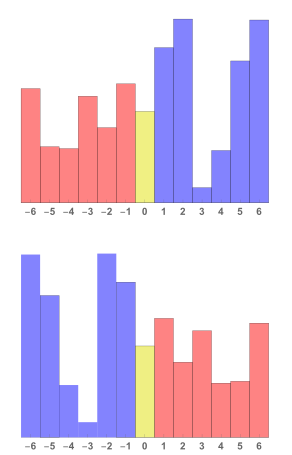
\includegraphics[width=\textwidth]{HL1dLattRefl0}
  \\ (even)
  \end{center}\end{minipage}
\qquad
  \begin{minipage}[b]{0.40\textwidth}\begin{center}
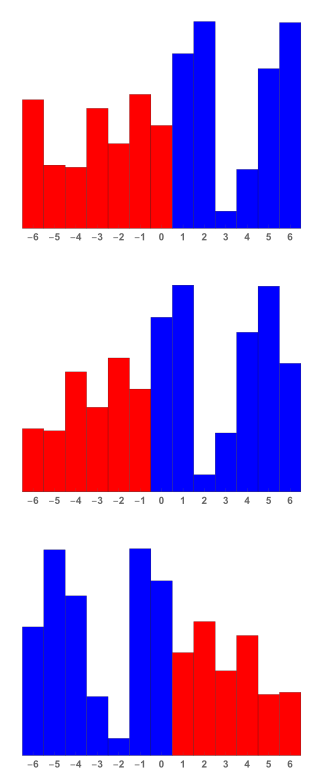
\includegraphics[width=\textwidth]{HL1dLattRefl1}
  \\ (odd)
  \end{center} \end{minipage}
  \end{center}
  \caption{\label{fig:HL1dLattRefl}
(Color online)~~~
There are two classes %\refeq{DinftyClassRefl}
of {\lattstate} reflections,
even \refeq{1dLattRefl0} and odd \refeq{1dLattRefl1}.
% :
% even, across a lattice site, and odd, across the mid-point between
% a pair of adjacent lattice sites.
    (Even)
reflection $\Refl$ exchanges (blue
$\ssp_j$) $\leftrightarrow$  (red $\ssp_{-j}$) %, $j>0$,
while leaving the yellow
field $\sitebox{\ssp_0}$ at lattice site ${0}$ fixed.
    (Odd)
reflection $\Refl_1=\Refl\shift$ swaps the
`blues' and the `reds' by a lattice
translation $\Xx\to\shift\Xx$, followed by a reflection $\Refl$. The
result is a reflection across the midpoint of the [01] interval,  marked
`|'.
See \reffig{LC21FieldConfig}\,(b) for the notation.
% Horizontal: lattice sites $j\in\integers$. Vertical: lattice site
% fields $\ssp_j$, labeled by their values before the reflection.
}
\end{figure}
%%%%%%%%%%%%%%%%%%%%%%%%%%%%%%%%%%%%%%%%%%%%%%%%%%%%%%%%%%%%%%%


\paragraph{Even class.}
Take $\Refl=\Refl_0$ as a representative of all even reflections
$\Refl_{2m}$,  and act on a {\lattstate} \refeq{1dLattStat}:
\bea
\Xx &=&
\cdots {\ssp}_{-3} {\ssp}_{-2}\,{\ssp}_{-1}\,
       {\ssp}_0\,
      {\ssp}_{1} {\ssp}_{2} {\ssp}_{3} {\ssp}_{4}  \cdots
\continue
\Refl\Xx &=&
\cdots  {\ssp}_{5} {\ssp}_{4} {\ssp}_{3} {\ssp}_{2} {\ssp}_{1}
       \sitebox{{\ssp}_0}\,
      {\ssp}_{-1} {\ssp}_{-2} {\ssp}_{-3}  \cdots
\,,
\label{1dLattRefl0}
\eea
with
\(
\sitebox{{\ssp}_0}
\)
indicating that the field at the lattice site $0$ is
unchanged by the reflection, see \reffig{fig:HL1dLattRefl}\,(even).

\paragraph{Odd class.}
 Take $\Refl_1$ as a representative of all odd reflections
$\Refl_{2m+1}$.
The result is:
\bea
\Xx &=& ~~~~\,
\cdots {\ssp}_{-3} {\ssp}_{-2} {\ssp}_{-1}
       \,{\underline {\ssp}}{}_0\,\,
      {\ssp}_{1} {\ssp}_{2} {\ssp}_{3} {\ssp}_{4}  \cdots
\continue
\shift\Xx &=& ~\,
\cdots {\ssp}_{-3} {\ssp}_{-2} {\ssp}_{-1}
       {\ssp}_0\,{\underline {\ssp}}{}_{1}\,\,
       {\ssp}_{2} {\ssp}_{3} {\ssp}_{4}  {\ssp}_{5} \cdots
\continue
\Refl_1\Xx =
\Refl\shift\Xx &=& ~~~~
\cdots  {\ssp}_{6} {\ssp}_{5} {\ssp}_{4} {\ssp}_{3} {\ssp}_{2} \,
      {\underline {\ssp}}{}_{1} | \, {\ssp}_0
      {\ssp}_{-1} {\ssp}_{-2} {\ssp}_{-3} \cdots
\,,
\label{1dLattRefl1}
\eea
where ${\underline {\ssp}}{}_{j}$ indicates the field value at the
lattice site $0$, and
\(
|
\)
indicates a reflection across midpoint
between lattice sites $0$ and $1$, see \reffig{fig:HL1dLattRefl}\,(odd).

More generally, one can say that the index $k$ in the
`translate-reflection' \refeq{Refl_k} operation
\(\Refl_{k} =\Refl\shift_k\)
advances the reflection point by $k/2$ steps, and then reflects
across it.
    \PC{2021-08-17} {
    Before publication, fine tune \reffig{fig:HL1dLattRefl}
    using LaTex, as in  \reffig{fig:1dLattRefl}.
    }

If you do not find the two kinds of reflections intuitive, the
distinction becomes crystal clear once you have a look at the
smallest Bravais lattices,
lattices of periods 3 and 4, \reffig{fig:D3D4}.

%%%%%%%%%%%%%%%%%%%%%%%%%%%%%%%%%%%%%%%%%%%%%%%%%%%%%%%%%%%%%%%%%%%%%%%%%%
\subsection{Symmetries of a system and of its solutions}
\label{s:1dSubLattSymms}

What's the deal about classes?
A `class' is a refinement of our intuitive
notion that ``rotations are rotations, and translations are
translations.''
Translated into a more familiar language,
conjugation \refeq{conjugate} is central
to all of physics: a `law' $f(\Xx)$ is invariant if it
retains its form in all symmetry related coordinate frames,
\beq
f(\Xx)  =  \LieEl^{-1} f(\LieEl\,\Xx)
\,,
\label{dscr:L-inv}
\eeq
where $\LieEl$ is a representation  of group
element $\LieEl\in \Group$.
If this holds, we say that $\Group$ is the \emph{symmetry} of the system.

For example, the `temporal Bernoulli' defining equation
\refeq{1stepDiffEq}  retains its form under conjugation by any
$\Cn{\infty}$  translation \refeq{C_infty},
\beq
\shift_i({s}\ssp_{\zeit} - \ssp_{\zeit+1})\shift_i^{-1}
= ({s}\ssp_{\zeit+i} - \ssp_{\zeit+i+1})\shift_i^{-1}
= {s}\ssp_{\zeit} - \ssp_{\zeit+1}
\,,
\ee{invBern}
while the Euler–Lagrange second-order difference equations
\refeq{LC21:1dTempFT}, `{\templatt}', `{\henlatt}', and `temporal
{$\phi^4$} theory' defining equations \refeq{LC21:1dTemplatt},
\refeq{LC21:1dHenlatt} and \refeq{LC21:1dPhi4} retain their form also
under any  $\Dn{\infty}$ reflection,
    \PC{2021-08-22} {
    This is not quite right, one does not `conjugate' a vector $\ssp_j$.
    Not sure how to elegantly deal with $\ssp_{-\zeit}^k$ term. Could
    have defined actions, but that does not work for the Bernoulli
    \refeq{invBern}.
    }
\beq
\Refl_i(
  -\ssp_{\zeit+1} + \,{g}\,V'(\ssp_{\zeit})-\ssp_{\zeit-1}
         )\Refl_i^{-1}
= -\ssp_{-\zeit+1} + \,{g}\,V'(\ssp_{-\zeit}) -\ssp_{-\zeit-1}
\,.
\ee{invPhi4}


%%%%%%%%%%%%%%%%%%%%%%%%%%%%%%%%%%%%%%%%%%%%%%%%%%%%%
\begin{figure} \begin{center}
  \begin{minipage}[b]{0.33\textwidth}\begin{center}
{(1)}~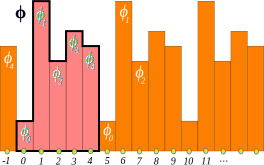
\includegraphics[width=\textwidth]{1dLatStatC_5_0}
\\
{($\shift_1$)}~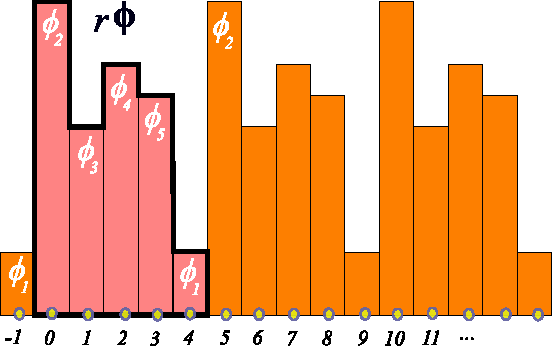
\includegraphics[width=\textwidth]{1dLatStatC_5_1}
\\
{($\shift_2$)}~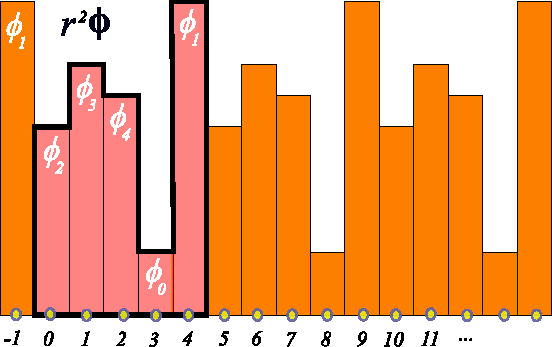
\includegraphics[width=\textwidth]{1dLatStatC_5_2}
\\
{($\shift_3$)}~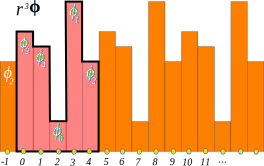
\includegraphics[width=\textwidth]{1dLatStatC_5_3}
\\
{($\shift_4$)}~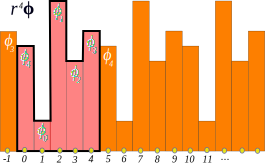
\includegraphics[width=\textwidth]{1dLatStatC_5_4}
  \end{center}\end{minipage}
\qquad\quad
  \begin{minipage}[b]{0.33\textwidth}\begin{center}
{($\Refl$)}~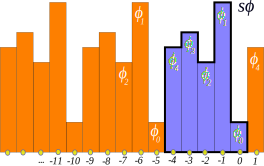
\includegraphics[width=\textwidth]{1dLatStatC_5_s0}
\\
{($\Refl_1$)}~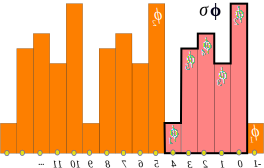
\includegraphics[width=\textwidth]{1dLatStatC_5_s1}
\\
{($\Refl_2$)}~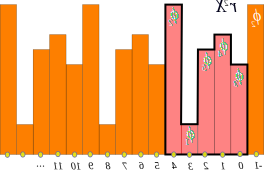
\includegraphics[width=\textwidth]{1dLatStatC_5_s2}
\\
{($\Refl_3$)}~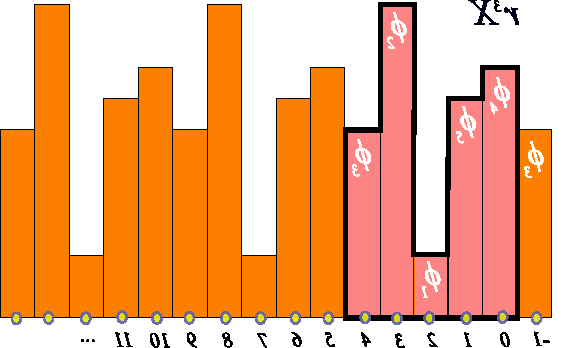
\includegraphics[width=\textwidth]{1dLatStatC_5_s3}
\\
{($\Refl_4$)}~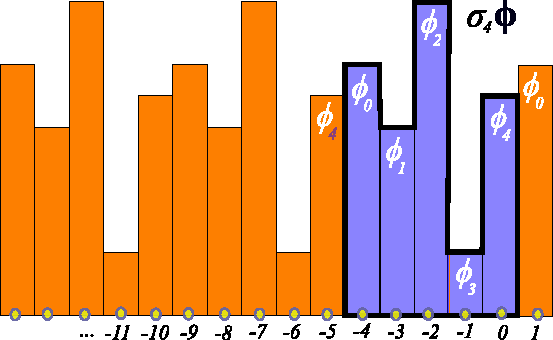
\includegraphics[width=\textwidth]{1dLatStatC_5_s4}

  \end{center} \end{minipage}
  \end{center}
  \caption{\label{fig:1dLatStatC_5}
(Color online)~~~
%Horizontal circles: \lattice\ lattice sites labelled by $\zeit\in\integers$.
%Vertical: the value of field $\ssp_\zeit$, plotted as a bar centred at
%lattice site $\zeit$.
(1)
A Bravais cell $\mathbf{a}$ with asymmetric
{\lattstate}
% \refeq{1dLattStatC_n}
\(\Xx=\cycle{\ssp_0 \ssp_1 \ssp_2 \ssp_3 \ssp_4}\),
no reflection symmetry, outlined in bold, invariant under the
translation subgroup $H_{5}$.
Its \Cn{\infty} orbit are the $\cl{}=5$ distinct {\lattstate}s (1) to
($\shift_4$), obtained by all of the $\Cn{5}$ translations.
Its \Dn{\infty}-orbit are $2\cl{}=10$ distinct {\lattstate}s,
5 translations (1) to ($\shift_4$)
and
5 translate-reflections ($\Refl$) to ($\Refl_4$), obtained by
all of the $\Dn{5}$ actions.
See \reffig{LC21FieldConfig}\,(b) for the notation.
Continued in \reffig{fig:symmLattStates}.
          }
\end{figure}
%%%%%%%%%%%%%%%%%%%%%%%%%%%%%%%%%%%%%%%%%%%%%%%%%%%%%

Given that $\Group$ is the {symmetry} of the system does not mean that
$\Group$ is also the symmetry of its solutions, or what we here call {\em
\lattstate}s.
They can satisfy
all of system's symmetries, a subgroup of them, or have no symmetry at
all.
For example, a generic {\lattstate} \refeq{1dLattStat} sketched in
\reffig{fig:HL1dLattRefl} has no symmetry beyond the identity, so its
symmetry group is the trivial subgroup $\{e\}$; any translation
$\shift_j$ or reflection $\Refl_k$ maps it into a different, distinct
{\lattstate}, as shown in \reffig{fig:1dLatStatC_5}.
At the other extreme, the constant {\lattstate}
$\ssp_j=\ssp$ is invariant under any translation or reflections - its
symmetry group is the full \Group, the symmetry of the system. In
between, there are {\lattstate}s whose symmetry is any subgroup of
$\Group$.

%%%%%%%%%%%%%%%%%%%%%%%%%%%%%%%%%%%%%%%%%%%%%%%%%%%%%%%%
\subsection{What are `{\lattstate}s'? Orbits?}
\label{s:LattStates}

Remember, for evolution-in-time, every period-\cl{}\ periodic point is a
fixed point of the \cl{}th iterate of the 1 time-step map. In the lattice
formulation, the totality of finite-period {\lattstate}s is the \emph{set
of fixed points} of all  $H_{\mathbf{a}}$ and  $H_{\mathbf{a},k}$
subgroups of $\Dn{\infty}$.

You can visualize a {\lattstate} invariant under (`fixed by') subgroup
$H_{\mathbf{a},k}$ as a tiling of the lattice $\integers$ by a
{\lattstate} tile of length \cl{}, symmetric under reflection $\Refl_k$,
see \reffig{fig:symmLattStates}\,(b-c).

    \begin{quote}
Definition: {\em
{\em Orbit} or \emph{$\Group$-orbit} of a {\lattstate} $\Xx$ is the
set of all {\lattstate}s
\beq
    \pS_\Xx = \{\LieEl\,\Xx \mid \LieEl \in {\Group}\}
\ee{GroupOrbDisc}
into which $\Xx$ is mapped under the action of group $\Group$.
We label the orbit $\pS_\Xx$ by any {\lattstate} $\Xx$ belonging to
it.
            }
    \end{quote}
As an example, the $\Dn{\infty}$ orbit of the period-5 {\lattstate}
% \refeq{1dLattStatC_n}
% \(\cycle{\ssp_0 \ssp_1 \ssp_2 \ssp_3 \ssp_4}\)
is shown in \reffig{fig:1dLatStatC_5}.
    \PC{2021-09-05} {
    This "maximal subgroup" does not seem to me to be defined here.
    Clean up!
    }
    \begin{quote}
Definition: Symmetry of a solution.
{\em
We shall refer to the maximal subgroup $\Group_\Xx \subseteq  \Group$ of
actions on {\lattstate}s within the orbit $\pS_\Xx$, which leave
the orbit invariant, as the \emph{symmetry}
$\Group_\Xx$ of the orbit $\pS_\Xx$,
\beq
\Group_\Xx =
   \{ \LieEl \in \Group_\Xx \mid \LieEl \Xx \in \pS_\Xx
   %,\,    \LieEl \ssp \neq \ssp  \mbox{ for } \LieEl \neq e
   \}
\,.
\ee{LC21:stabilSet}
}
    \end{quote}
An orbit $\pS_\Xx$ is $\Group_\Xx$-{\em symmetric}
({\em symmetric}, {\em set-wise symmetric}, {\em self-dual})
if the action of elements of $\Group_\Xx$ on
the set of {\lattstate}s $\pS_\Xx$ reproduces the orbit.
%
% \item[2021-07-28 Predrag]
% Rather than Lind's nebulous `index'\rf{Lind96}, for $|\Group/{H}|$ in
% \refeq{Ryu17eq:1.3}
    \begin{quote}
Definition: Multiplicity
{\em
of orbit $\pS_\Xx$ is given by
}
\beq
m_\Xx=|\Group|/|\Group_{\Xx}|
\,.
\ee{GroupOrbMult}
    \end{quote}
(See \toChaosBook{section*.166} {p.~166}.)



\bigskip

And now, a pleasant surprise, obvious upon an inspection of
\reffigs{fig:1dLatStatC_5}{fig:symmLattStates}: what happens
in the Bravais cell, stays in the Bravais cell.
Even though
the lattices \lattice, $\lattice_{\mathbf{a}}$ are infinite,
and their symmetries
$\Dn{\infty}$, $H_{\mathbf{a}}$, $H_{\mathbf{a},k}$ are
\emph{infinite} groups, the Bravais {\lattstate}s'
\emph{orbits} are \emph{finite}, described by the finite group
permutations of the infinite lattice curled up into a Bravais cell periodic
$\cl{}$-site ring.


%\subsection{Finite groups}
%\label{s:1dmnFntPer}


%%%%%%%%%%%%%%%%%%%%%%%%%%%%%%%%%%%%%%%%%%%%%%%%%%%%%%%%%%%%%%%%%%
% PC 2021-08-05:  from ChaosBook book/figs/D3.tex, D3.tex
\begin{figure} \begin{center}
  \begin{minipage}[b]{0.32\textwidth}\begin{center}
  \setlength{\unitlength}{1.00\textwidth}
  \begin{picture}(1,1.12469246)%
    \setlength\tabcolsep{0pt}%
    \put(0,0){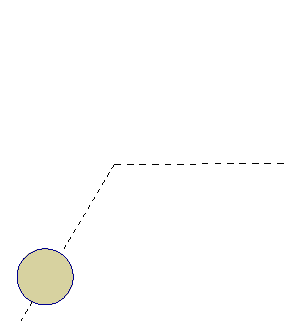
\includegraphics[width=\unitlength,page=1]{D3}}%
    \put(0.23496893,0.6474626){\color[rgb]{0.1372549,0.12156863,0.1254902}\makebox(0,0)[lt]{\smash{$\shift$}}}%
    \put(0,0){\includegraphics[width=\unitlength,page=2]{D3}}%
    \put(0.34167143,0.39068967){\color[rgb]{0.1372549,0.12156863,0.1254902}\makebox(0,0)[lt]{\smash{$\shift_2$}}}%
    \put(0.05464421,0.6373038){\color[rgb]{0.1372549,0.12156863,0.1254902}\makebox(0,0)[lt]{\smash{$\Refl$}}}%
    \put(0.67969793,0.84532127){\color[rgb]{0.1372549,0.12156863,0.1254902}\makebox(0,0)[lt]{\smash{$\Refl_1$}}}%
    \put(0.44996833,0.19132446){\color[rgb]{0.1372549,0.12156863,0.1254902}\makebox(0,0)[lt]{\smash{$\Refl_2$}}}%
    \put(0,0){\includegraphics[width=\unitlength,page=3]{D3}}%
    \put(0.6357866,0.31003627){\color[rgb]{0,0,0}\makebox(0,0)[lt]{\smash{$\pSRed$}}}%
    \put(0.81616715,0.52920775){\color[rgb]{1,1,1}\makebox(0,0)[lt]{\smash{{\Large 0}}}}%
    \put(0.12429459,0.92867118){\color[rgb]{1,1,1}\makebox(0,0)[lt]{\smash{{\Large 1}}}}%
    \put(0.12402384,0.13559257){\color[rgb]{1,1,1}\makebox(0,0)[lt]{\smash{{\Large 2}}}}%
    \put(0,0){\includegraphics[width=\unitlength,page=4]{D3}}%
  \end{picture} \\ $(o)$
  \end{center}\end{minipage}
\qquad
  \begin{minipage}[b]{0.39\textwidth}\begin{center}
  \setlength{\unitlength}{1.00\textwidth}
  \begin{picture}(1,0.94270725)%
    \setlength\tabcolsep{0pt}%
    \put(0,0){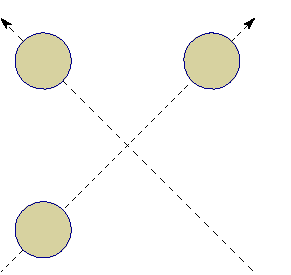
\includegraphics[width=\unitlength,page=1]{D4}}%
    \put(0.11589164,0.70318699){\color[rgb]{1,1,1}\makebox(0,0)[lt]{\smash{{\Large 2}}}}%
    \put(0.11465857,0.11853823){\color[rgb]{1,1,1}\makebox(0,0)[lt]{\smash{{\Large 3
    }}}}%
    \put(0,0){\includegraphics[width=\unitlength,page=2]{D4}}%
    \put(0.69662672,0.11848457){\color[rgb]{1,1,1}\makebox(0,0)[lt]{\smash{{\Large 0}}}}%
    \put(0.69785979,0.70163221){\color[rgb]{1,1,1}\makebox(0,0)[lt]{\smash{{\Large 1}}}}%
    \put(0.48887673,0.58974203){\color[rgb]{0.1372549,0.12156863,0.1254902}\makebox(0,0)[lt]{\smash{$\shift_1$}}}%
    \put(0,0){\includegraphics[width=\unitlength,page=3]{D4}}%
    \put(0.24073374,0.49925981){\color[rgb]{0.1372549,0.12156863,0.1254902}\makebox(0,0)[lt]{\smash{$\shift_2$}}}%
    \put(0.33991763,0.28480816){\color[rgb]{0.1372549,0.12156863,0.1254902}\makebox(0,0)[lt]{\smash{$\shift_3$}}}%
    \put(0.95378545,0.34914366){\color[rgb]{0.1372549,0.12156863,0.1254902}\makebox(0,0)[lt]{\smash{$\Refl_1$}}}%
    \put(0.87112523,0.73973783){\color[rgb]{0.1372549,0.12156863,0.1254902}\makebox(0,0)[lt]{\smash{$\Refl_2$}}}%
    \put(0.50562029,0.87631462){\color[rgb]{0.1372549,0.12156863,0.1254902}\makebox(0,0)[lt]{\smash{$\Refl_3$}}}%
    \put(0.11826698,0.87765494){\color[rgb]{0.1372549,0.12156863,0.1254902}\makebox(0,0)[lt]{\smash{$\Refl$}}}%
    \put(0,0){\includegraphics[width=\unitlength,page=4]{D4}}%
  \end{picture}  \\ $(e)$
  \end{center} \end{minipage}
  \end{center}
  \caption{\label{fig:D3D4}
% Dihedral group \Dn{3}: \Dn{4}:
Translational and rotational symmetries of
    $(o)$
an equilateral triangle,  $\cl{}=3$ lattice sites;
    $(e)$
a square,                  $\cl{}=4$ lattice sites.
The $\cl{}$ rotations $\shift_j$ and the $\cl{}$ translate-reflect
$\Refl_k$ (elements of dihedral group \Dn{\cl{}} \refeq{DnElements},
even reflection axes dashed, odd reflections full line)
overly an $\cl{}$-sided regular polygon onto itself. They
also tile it with  the $2\cl{}$ copies $\pSRed_\ell$ of the fundamental
domain, indicated by the shaded wedge.
}
\end{figure}
%%%%%%%%%%%%%%%%%%%%%%%%%%%%%%%%%%%%%%%%%%%%%%%%%%%%%%%%%%%%%%%

Indeed, to grasp everything one needs to know about translations
$\shift_j$ (for regular polygons, `rotations'),
and
reflections $\Refl_k$,
it suffices to understand the symmetries of
an equilateral triangle (dihedral group \Dn{3})
and
a square (dihedral group \Dn{4}), depicted in \reffig{fig:D3D4}.
It is clear by inspection that an $\cl{}$-sided regular polygon has
$\cl{}$-fold translational symmetry and $\cl{}$ reflection symmetry axes.
The group of such symmetries is the finite dihedral group
\beq
\Dn{\cl{}} = \{1,\Refl,\shift,\Refl_{1},\shift_{2},\Refl_{2},\
           \cdots,
           \shift_{\cl{}-1},\Refl_{\cl{}-1}\}
%\,,
\ee{DnElements}
of order $2\cl{}$.
A half of its elements are the $\cl{}$ cyclic group \Cn{n} translations
$\shift_{j}$.
% 2\pi/n,2\cdot2\pi/n,\cdots$,
The other half are the $\cl{}$ reflections $\Refl_k$, one for the
reflection across each symmetry axis.
The group multiplication table is the same as the $\Dn{\infty}$
\refeq{eq:DinftyMultTab}, but with all subscripts mod $\cl{}$.
%
As in \refeq{DinftyInversion},
conjugation by any reflection reverses the direction of translation
\beq
   \Refl_i\shift_j\Refl_{-i} =  \shift_{\cl{}-j}
\,,\qquad 0<j<\cl{}
\,,
\ee{D_nInversion}now mod $\cl{}$,
so every translation pairs up with the equal counter-translation to form
a 2-element class \refeq{DinftyClassShift}. %$\{\shift_j,\shift_{\cl{}-j}\}$.

The distinction between the classes of even and odd reflections
\refeq{DinftyClassRefl} is visually self-evident by inspection of
\reffig{fig:D3D4}:
the symmetry axes either connect opposite lattice sites, or bisect the
edges, or both, if $\cl{}$ is odd (a triangle, for example).
One can say that the index $k$ in the
`translate-reflection' \refeq{Refl_k} operation
\(
\Refl_{k} %=\Refl\shift_k\,.
\) advances the reflection point by $k$ 1/2 steps, and then reflects
across it.

For a polygon with an \emph{odd} number of
lattice sites (a triangle, for example), we see by contemplating the
triangle of \reffig{fig:D3D4},  as well as by taking  mod $\cl{}$ of the
conjugation relation \refeq{D_nConj}, that
% for  $\cl{}$ odd, the
all reflections are in the same conjugacy class $\{\Refl_{j}\}$:
 there is no splitting into odd and even cases, in
contrast to the infinite lattice case \refeq{DinftyClassRefl}.

For a polygon with an \emph{even} number of lattice sites (a square, for
example), one must distinguish
the `long' axes that connect lattice sites (we label them by even numbers
$0,2,\cdots$)
from
the `short' symmetry axes that bisect opposite edges (labelled by odd
numbers $1,3,\cdots$).
%
The corresponding reflections belong to
different \Dn{\cl{}} (subclasses of
\refeq{DinftyClassRefl}),
\bea
\mbox{even reflections}
    &&\quad
\{\Refl,\Refl_{2},\Refl_{4},\cdots,\Refl_{\cl{}/2}\}
    \continue
\mbox{odd reflections}
    &&\quad
\{\Refl_{1},\Refl_{3},\cdots,\Refl_{\cl{}/2+1}\}
\,.
\label{DnClassRefl}
\eea

%%%%%%%%%%%%%%%%%%%%%%%%%%%%%%%%%%%%%%%%%%%%%%%%%%%%%%%%
\subsection{Symmetries of {\lattstate}s}
\label{s:LattStateSyms}


%%%%%%%%%%%%%%%%%%%%%%%%%%%%%%%%%%%%%%%%%%%%%%%%%%%%%
\begin{figure}
  \centering
{$(a)$}
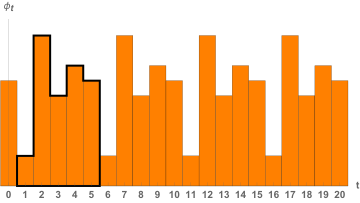
\includegraphics[width=0.40\textwidth]{HL1dLatticeStateBar1}\quad
{$(o)$}
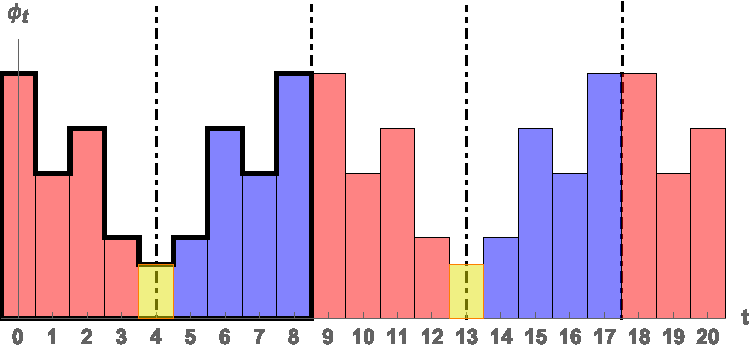
\includegraphics[width=0.40\textwidth]{HL1dLatticeStateBar2}
\\ %~~~
{$(ee)$}
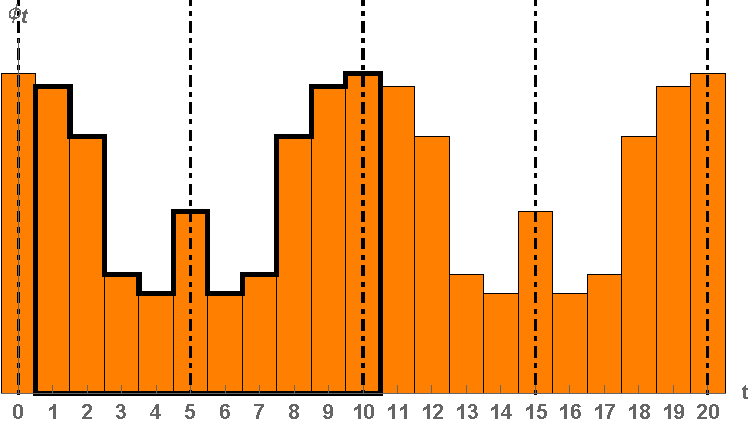
\includegraphics[width=0.40\textwidth]{HL1dLatticeStateBar4}\quad
{$(eo)$}
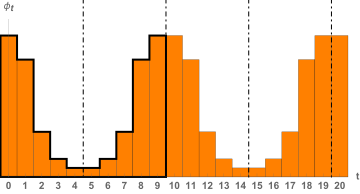
\includegraphics[width=0.40\textwidth]{HL1dLatticeStateBar3}

  \caption{\label{fig:symmLattStates}
(Color online)~~~
A Bravais {\lattstate} \Xx\ has one of the
4 possible symmetries, illustrated by:
$(a)$ {\em No reflection symmetry:}
    an $H_{5}$ invariant period-5 {\lattstate} \refeq{reflSymNo}. For its
    \Group-orbit, see \reffig{fig:1dLatStatC_5}.
$(o)$ {\em Odd period, reflection-symmetric:}
    an $H_{9,8}$ invariant period-9 {\lattstate} \refeq{reflSymOdd},
    %PC 2021-08-21 checked
    reflection symmetric over the lattice sites interval [8-9]  midpoint
    and over the lattice site~4.
$(ee)$ {\em Even period, even reflection-symmetric:}
    an $H_{10,0}$  invariant period-10 {\lattstate} \refeq{reflSymEvens0},
    reflection symmetric over lattice sites 0 and 5.
$(eo)$ {\em Even period, odd reflection-symmetric:}
    an $H_{10,9}$  invariant period-10 {\lattstate} \refeq{reflSymEvens1},
    reflection symmetric over the [4-5] and [9-10] interval midpoints.
Horizontal: lattice sites labelled by $\zeit\in\integers$.
Vertical: value of field $\ssp_\zeit$, plotted as a bar centred at
lattice site $\zeit$.
Even reflection axes dashed, odd reflections full line.
          }
\end{figure}
%%%%%%%%%%%%%%%%%%%%%%%%%%%%%%%%%%%%%%%%%%%%%%%%%%%%%

A Bravais {\lattstate} \Xx\ has one of the
four symmetries:

\bea
    && \mbox{ asymmetric, no reflection symmetry }
    \continue
(a) \quad &&
\cycle{\ssp_0 \ssp_1 \ssp_2 \ssp_3 \cdots \ssp_{\cl{}-1}}
\label{reflSymNo} \\ % the same as {1dLattStatC_n}
    &&
\mbox{ multiplicity } m_\Xx=2\cl{}
    \nnu %\,,
\eea
{\lattstate} invariant under the translation group
$H_{\cl{}}$.
Its \Group-orbit, generated by all actions of \Dn{\infty},
results  in  $2\cl{}$ distinct,  \Dn{\cl{}} related {\lattstate}s.
This is illustrated by the $H_{5}$-invariant {\lattstate} \Xx\ of
\reffig{fig:1dLatStatC_5}. %{fig:symmLattStates}\,$(a)$.
Its \Dn{5} orbit are $2\cl{}=10$ {\lattstate}s, 5  translations
and 5 translate-reflections.
    \PC{2021-08-20} {
    Merge \reffig{fig:symmLattStates}\,$(a)$ with
    \emph{1dLatStatC\_5\_0x3.svg}.
    }

Next, the reflection-symmetric {\lattstate}s.
As illustrated in \reffigs{fig:HL1dLattRefl}{fig:D3D4},
there are two classes \refeq{DinftyClassRefl} of {\lattstate} reflections:
even, across a lattice site, and
odd, across the mid-point between a pair of adjacent lattice sites.
However, as is evident by inspection of \reffig{fig:D3D4}, curling up the
lattice {\lattice} into a Bravais cell periodic $\cl{}$-site ring
implies that an axis cuts the ring twice, and
constrains the possible reflection points to three configurations:

\bea
    && \mbox{ odd period } \cl{}=2m+1
    \continue
(o) \quad &&
\cycle{\sitebox{\ssp_0} \ssp_1 \ssp_2 \cdots \ssp_{m}|\ssp_{m}\cdots \ssp_2 \ssp_1}
\label{reflSymOdd} \\
    &&
\mbox{ multiplicity } m_\Xx=\cl{}
    \nnu %\,,
\eea
{\lattstate} invariant under the dihedral group $H_{\cl{},k}$,
illustrated by the $H_{9,8}$ invariant {\lattstate} \Xx\
of \reffig{fig:symmLattStates}\,$(o)$.
% as well as by the triangle of \reffig{fig:D3D4}\,(1)).
\bea
    && \mbox{ even period } \cl{}=2m+2\,, \mbox{ even reflection } k
    \continue
(ee) \quad &&
\cycle{\sitebox{\ssp_0} \ssp_1 \ssp_2 \cdots \ssp_{m}
        \sitebox{\ssp_{m+1}} \ssp_{m} \cdots \ssp_2 \ssp_1}
\label{reflSymEvens0} \\
    &&
\mbox{ multiplicity } m_\Xx=\cl{}/2
    \nnu %\,,
\eea
{\lattstate} invariant under the dihedral group $H_{\cl{},k}$,
$k$ even,
illustrated by the $H_{10,0}$ invariant {\lattstate} \Xx\
of \reffig{fig:symmLattStates}\,$(ee)$.
\bea
    && \mbox{ even period } \cl{}=2m\,, \mbox{ odd reflection } k
    \continue
(eo) \quad &&
\cycle{\ssp_1 \ssp_2 \ssp_3 \cdots \ssp_{m}| \ssp_{m}\cdots \ssp_2 \ssp_1|}
\label{reflSymEvens1} \\
    &&
\mbox{ multiplicity } m_\Xx=\cl{}/2
    \nnu %\,,
\eea
{\lattstate} invariant under the dihedral group $H_{\cl{},k}$,
$k$ odd,
illustrated by the $H_{10,9}$ invariant {\lattstate} \Xx\
of \reffig{fig:symmLattStates}\,$(eo)$.

For long periods $\cl{}$, almost all orbits are of no-symmetry type
\refeq{reflSymNo}.
So why do we care about the symmetric orbits so much? The reason is that
the \po\ expansions are dominated by the short orbits, and many, if not
the most of those are reflection-symmetric.

The {\lattstate} {symmetry} $\Group_\Xx$ \refeq{LC21:stabilSet} of the
above $(o)$--$(eo)$ reflection-symmetric {\lattstate}s \Xx\ is the reflection
group $\Dn{1}=\{1,\Refl_k\}$, but we will spare the reader the
group-theorist's cosets and group quotients. For us, this symmetry means
two things:
\begin{itemize}
  \item[(1)]
The \Dn{\infty} orbits of reflection-symmetric {\lattstate}s contain only
translations, as any reflection amounts to a cyclic group
\Cn{\cl{}} translation.
(Try reflecting a  {\lattstate} in \reffig{fig:symmLattStates}\,(b-d)
over any lattice site or mid-interval.)
  \item[(2)]
The prime {\lattstate} is a `half' of the Bravais cell,
give or take some boundary sites, the length ${m}$ orbit,
\beq
\tilde{\Xx}      = \ssp_1 \ssp_2 \ssp_3 \cdots \ssp_{m}
\,.
\ee{primeLattStat}


\end{itemize}
Reflection breaks the translational invariance, and how one reconstructs
the period-$\cl{}$ orbit from this length-$m$ \brick\ is a bit tricky. To
develop intuition about that, it is helpful to have a look at
explicit matrix
representations of $\Dn{\cl{}}$ operations.

%%%%%%%%%%%%%%%%%%%%%%%%%%%%%%%%%%%%%%%%%%%%%%%%%%%%%%%%%%%%%%%%%%%%%%%%%%
\subsection{Permutation representation}
\label{sect:permReps}

A {\lattstate} {\Xx} over a Bravais cell $\mathbf{a}$ can be assembled
into an $\cl{}$\dmn\ vector whose components are lattice site fields
\beq
\transp{\Xx} = (\ssp_0,\ssp_1,\ssp_2,\ssp_3,\cdots,\ssp_{\cl{}-1})
\,,
\ee{1dLattStatVec}
with the first field in such vector placed at the lattice site 0, the
second at the lattice site 1, and so on. Matrices that reshuffle the
components of such vectors form the {\em permutation representation} of a
finite group \Group, which gives us a different and helpful
perspective on the three kinds of symmetric solutions of the preceding
section.

The permutation representation of 1-step lattice translation $\shift$
acts on a Bravais {\lattstate} by the off-diagonal
$[\cl{}\!\times\!\cl{}]$ matrix \refeq{hopMatrix}. This is a cyclic
\Cn{\cl{}} permutation that translates the {\lattstate} $\Xx$
"for\-ward-in-time" by one site,
\[
\transp{(\shift\Xx)}=(\ssp_1,\ssp_2,\cdots,\ssp_{\cl{}-1},\ssp_0)
\,.
\]
A permutation representation of a \Dn{\cl{}} translate-reflect operation
is essentially an anti-diagonal matrix that reverses the order of site
fields, up to a cyclic permutation
\[
\transp{(\Refl_k\Xx)}=(\ssp_{\cl{}-1},\cdots,\ssp_2,\ssp_1,\ssp_0)
\,.
\]
Symmetries of triangles and squares, \reffig{fig:D3D4}, help us make this
precise.

%     \item[2021-03-09 Han]
\emph{Odd period}:
In odd dimensions, the $\cl{}$ translate-reflect matrices of \Dn{\cl{}} are
related by translations \refeq{D_nConj}.
For example, for a period-3 {\lattstate}
without symmetry
\(
\transp{\Xx} = (\ssp_0,\ssp_1,\ssp_2)
\,,
\)
they are
\[
\Refl=
\left(
\begin{array}{ccc}
 1 & 0 & 0 \\
 0 & 0 & 1 \\
 0 & 1 & 0
\end{array}
\right)
    \,,\quad
{\Refl_1}=
\left(
\begin{array}{ccc}
 0 & 1 & 0 \\
 1 & 0 & 0 \\
 0 & 0 & 1
\end{array}
\right)
    \,,\quad
\Refl_2=
\left(
\begin{array}{ccc}
 0 & 0 & 1 \\
 0 & 1 & 0 \\
 1 & 0 & 0
\end{array}
\right)
\,.
\]
In agreement with \refeq{reflSymOdd}, \reffig{fig:D3D4}\,$(o)$ and
\reffig{fig:symmLattStates}\,$(o)$, reflections keep one lattice site fixed
(for each permutation matrix $\Refl_k$ there is only one `1' on the
diagonal), swap the rest.

Next consider a period-5 reflection symmetric {\lattstate}s tiles the infinite lattice
\lattice\ with a reflection-fixed $\sitebox{\ssp_0}$, and a length-2
{\brick} $(\ssp_1,\ssp_2)$,
\beq
\Xx =
\cdots \ssp_2 \ssp_1 \sitebox{\ssp_0} \ssp_1 \ssp_2 |
      \ssp_2 \ssp_1 \sitebox{\ssp_0} \ssp_1 \ssp_2 |\cdots
\,.
\ee{symmCycD5}
\Dn{5} permutation representation of reflections of a pentagon, illustrates that
fixpoints {\Xx} of $\Refl_{k}$ are cyclicly related:
\bea
\Refl\Xx &=&
\left(
\begin{array}{ccccc}
 1 & 0 & 0 & 0 & 0 \\
 0 & 0 & 0 & 0 & 1 \\
 0 & 0 & 0 & 1 & 0 \\
 0 & 0 & 1 & 0 & 0 \\
 0 & 1 & 0 & 0 & 0
\end{array}
\right)
\left(\begin{array}{c}
 \sitebox{\ssp_0}\cr
 \ssp_1\cr
 \ssp_2\cr
 \ssp_2\cr
 \ssp_1\cr
\end{array}\right)
=
\left(\begin{array}{c}
 \sitebox{\ssp_0}\cr
 \ssp_1\cr
 \ssp_2\cr
 \ssp_2\cr
 \ssp_1\cr
\end{array}\right)
        \continue
\Refl_{4}(\shift_{-2}\Xx )
     &=&
\left(
\begin{array}{ccccc}
 0 & 0 & 0 & 0 & 1 \\
 0 & 0 & 0 & 1 & 0 \\
 0 & 0 & 1 & 0 & 0 \\
 0 & 1 & 0 & 0 & 0\\
 1 & 0 & 0 & 0 & 0
\end{array}
\right)
\left(\begin{array}{c}
 \ssp_2\cr
 \ssp_1\cr
 \sitebox{\ssp_0}\cr
 \ssp_1\cr
 \ssp_2\cr
\end{array}\right)
=
\left(\begin{array}{c}
 \ssp_2\cr
 \ssp_1\cr
 \sitebox{\ssp_0}\cr
 \ssp_1\cr
 \ssp_2\cr
\end{array}\right)
\,.
\label{symmCycD5Refl}
\eea

The symmetry conditions are the Bravais lattice site 5-periodicity
mod 5, and the even reflection across
$\sitebox{\ssp_0}$:
\beq
\ssp_{i} = \ssp_{i+5}
    \,, \quad
\ssp_{-i} = \ssp_{i}
\,.
\ee{symmCycD5bcs}
A {\lattstate} satisfies
the defining equation \refeq{LC21:1dTempFT} %{catMapNewt}
\beq
- \ssp_{\zeit-1}  +  V'(\ssp_{\zeit}) - \ssp_{\zeit+1}
    =
\Ssym{\zeit}
\,,
\ee{LC21:1dTempFTa} %{catMapHL}
on the period-5 Bravais cell,
\bea
    V'(\ssp_{0}) - 2 \ssp_1 &=& m_0 \continue
-\ssp_0 +V'(\ssp_{1}) -\ssp_2 &=& m_1 \continue
-\ssp_1 +V'(\ssp_{2}) -\ssp_2 &=& m_2 \continue
-\ssp_1 +V'(\ssp_{2}) -\ssp_2 &=& m_2 \continue
-\ssp_0 +V'(\ssp_{1}) -\ssp_2 &=& m_1
\label{symmCycD5eqs5} % from {HLsymmCycD5eqs}
\eea
where we have used \refeq{symmCycD5bcs}.
The result is a symmetry reduced {\jacobianOrb}, with
rows modified by the \bcs,
\bea
    V'(\ssp_{0}) - 2 \ssp_1 &=& m_0 \continue
-\ssp_0 +V'(\ssp_{1}) -\ssp_2 &=& m_1 \continue
-\ssp_1 +V'(\ssp_{2}) -\ssp_2 &=& m_2
\label{symmCycD5eqs} % from {HLsymmCycD5eqs}
\eea
with a 3\dmn\ {\jacobianOrb} \refeq{jMorb1dFT}
\bea
\jMorb_+ &=&
\left(\begin{array}{ccc}
{s}_0 & -2 & 0 \\
 -1 & {s}_1 & -1 \\
 0 & -1 & {s}_2-1
\end{array}\right)
\,,
\label{OrbJacobianD5} % from {HLOrbJacobianD5}
\eea
At this point we have to abandon the detailed discussion of the four
kinds of symmetry reduced {\jacobianOrbs}: the message is that for any
reflection-symmetric Bravais cell the cyclic translational symmetry is
broken, and one has to impose the correct $\sitebox{\ssp_0}$ and odd $|$
reflection \bcs\ to define the {\jacobianOrb} for the \emph{prime} orbit.

%%%%%%%%%%%%%%%%%%%%%%%%%%%%%%%%%%%%%%%%%%%%%%%%%%%%%%%%%%%%%%%%%%%%%%%%%%
\subsection{Reciprocal lattice}
\label{sect:DnReciprLatt}


%%%%%%%%%%%%%%%%%%%%%%%%%%%%%%%%%%%%%%%%%%%%%%%%%%%
\begin{figure}
  \centering
              \begin{minipage}[c]{0.4\textwidth}\begin{center}
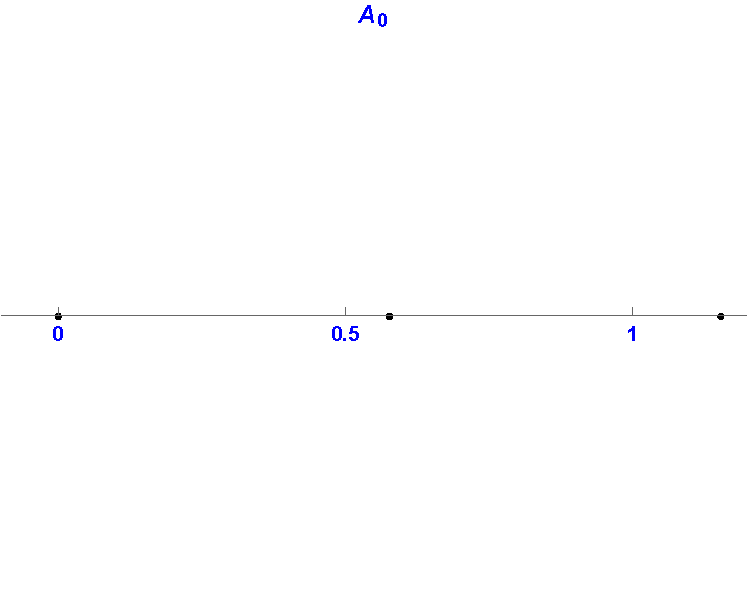
\includegraphics[width=1.0\textwidth]{HLCatmapD3a}\\(a)
            \end{center}\end{minipage}
            \begin{minipage}[c]{0.4\textwidth}\begin{center}
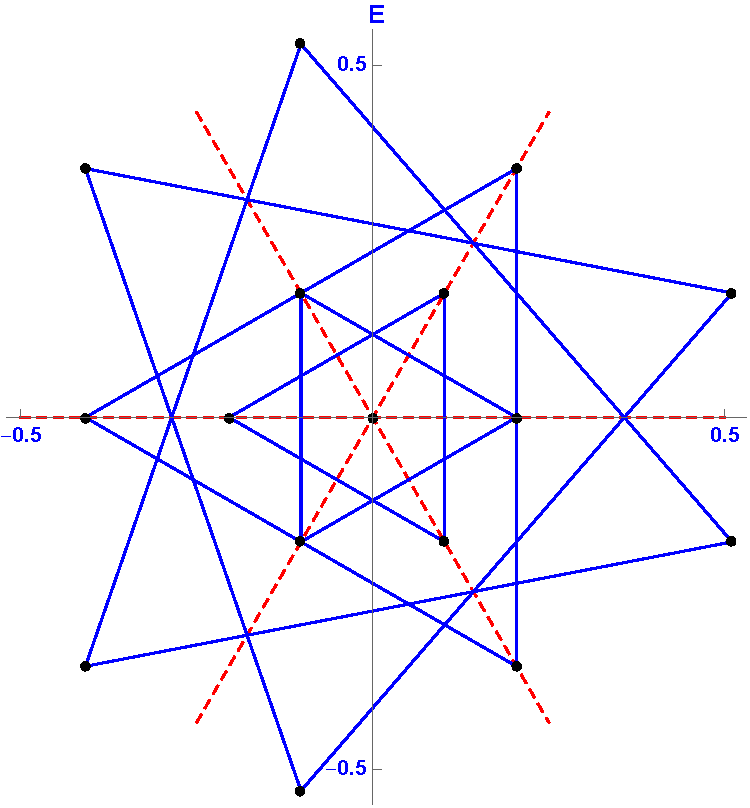
\includegraphics[width=1.0\textwidth]{HLCatmapD3b}\\(b)
            \end{center}\end{minipage}
  \caption{\label{fig:HLCatmapD3}
Period-3 {\lattstate}s of the $s=3$ \templatt, plotted in the $\Dn{3}$
permutation irreps subspaces $A_0+E$. In contrast with the
\Cn{\cl{}} complex irreps (see the \Cn{3} example
\reffig{fig:BernC3}), the 2\dmn\ irrep $E\in\reals^2$ is real.
In the subspace of the $E$ irrep,
{\lattstate}s that are related by cyclic permutations are connected by blue lines.
The 2 big triangles are a single \Dn{3} 6-{\lattstate}s orbit, what for
\Cn{3} is a pair of 3-{\lattstate}s orbits without time reversal symmetry.
The remaining 3 smaller triangles are 3 time-reversal symmetric orbits;
the pair in the middle is related by the field symmetry
 $\Dn{1}: S\ssp_i = 1-\ssp_i$ specific to
the \templatt, a symmetry not quotiented in this paper. The state in
the center is the fixed point.
Red dashed lines are the reflection axes of the $\Dn{3}$ group.
Note that there are 4 states
on each reflection axis.
}
\end{figure}
%%%%%%%%%%%%%%%%%%%%%%%%%%%%%%%%%%%%%%%%%%%%%%%%%%%

When we use the similarity transformation to diagonalize the permutation
representation, the {\lattstate}s are transformed into the subspaces of
the irreps. The example of period-3 {\lattstate}s of \templatt\ with
$s=3$ is shown in \reffig{fig:HLCatmapD3}. The permutation representation
is block diagonalized by basis vectors: $e_0=1/\sqrt{3}(1,1,1)$,
$e_1=\sqrt{2/3}(\cos(2\pi/3),\cos(4\pi/3),1)$ and
$e_2=\sqrt{2/3}(\sin(2\pi/3),\sin(4\pi/3),0)$. The basis vector $e_0$
spans the subspace of the 1\dmn\ irrep $A_0$. Basis vectors $e_1$ and
$e_2$ span the subspace of the 2\dmn\ irrep $E$.

Period-3 {\lattstate}s of cat map with $s=3$ are mapped into the subspace
of the irreps $A_0$ and $E$ in \reffig{fig:HLCatmapD3}.
The irrep $A_0$ is the symmetric 1\dmn\ irrep, so in the subspace of $A_0$ the components
of {\lattstate}s are invariant under the action of the $\Dn{3}$ group.
In the 2\dmn\ subspace of the irrep $E$, the shift operator $\shift$ rotates the
{\lattstate}s clockwise by $2\pi/3$, while the reflection operator $\Refl$ reflects the {\lattstate}s
over the axis passing through the origin and pointing toward $(\cos(2\pi/3),\sin(2\pi/3))$.
In \reffig{fig:HLCatmapD3}
{\lattstate}s that are related by shifts are connected by blue lines.
The red dashed lines are reflection axis of the reflection operators.
The 2 big triangles in \reffig{fig:HLCatmapD3} subspace of $E$ are lattice states
that belong to 2 orbits which are related by time reflection. The remaining 3 triangles
are lattice states from 3 orbits which are invariant under time reflection.

If the space of the field configuration has \Dn{\cl{}} symmetry,
the subspace of the 2\dmn\ irrep $E_1$ can be divided
into $2\cl{}$ copies by the irrep. One can choose the fundamental domain to be the region
with polar angle between 0 and $\pi/\cl{}$, assuming that the horizontal axis is one of the
reflection axis of the irrep $E_1$. Each orbit only appears once in the fundamental domain,
as shown in \reffig{fig:HLCatmapD3}. Note that the two orbits related by
the time reflection are considered one orbit of the dihedral group.

If, in addition, the law is time-reversal (or time-inversion) invariant,
the symmetry includes time-reflection, ie, it is dihedral group \Dn{n}
with 2$\cl{}$ elements, so the reciprocal lattice should be a half of the
above 1/$\cl{}$ sliver of a $\cl{}$-gon, and irreps are now either 1 or 2
dimensional. Even $\cl{}$ is different from odd $\cl{}$, and solutions either appear
in pairs, or are self dual under reflection in 3 different ways.

Due to the time
reversal, all $k={2\pi}/{5}$ irrep states are the same as the
$k={4\pi}/{5}$ irrep states.


\subsubsection{Fundamental domain}
What happens when {\lattstate}s appear on the boundary of the fundamental domain?
There are two possible situations. The first situation is that the {\lattstate} belongs to an
orbit with multiplicity less than the order of the symmetry group. For example,
in \reffig{fig:HLCatmapD3} subspace of $E$, there are 3 points in the fundamental domain
with polar angle equal to 0 or $\pi/3$. These 3 points are representative {\lattstate}s of orbits
with time reflection symmetry. The multiplicities of these orbits are 3 instead of 6.

The second situation is that the multiplicity of
the orbit of the {\lattstate} is equal to the order of the symmetry group
but the component in the subspace is 0. For example,
\[
\Xx = \frac{1}{104} (17, 51, 49, 43, 25, 75)
\]
is a period-6 {\lattstate} of the temporal Bernoulli
\refeq{LC21:1dBernLatt} with $s=3$. Using the discrete Fourier transform
this {\lattstate} becomes:
\[
\cssp =
\left(\frac{5}{2 \sqrt{6}},0,\frac{-5-3 i \sqrt{3}}{13
   \sqrt{6}},-\frac{\sqrt{3}}{4\sqrt{2}},\frac{-5+3 i \sqrt{3}}{13 \sqrt{6}},0\right) \,.
\]
This is a period-6 {\lattstate}. It belongs to an orbit that
contains 6 different {\lattstate}s. The $k=1$ component of this lattice
state is 0, which is on the boundary of the fundamental domain. To put this kind of
{\lattstate}s into the fundamental domain one needs to divide other subspaces.
For this lattice state the $k=2$ and $k=3$ components are not 0. The irreps divide
the $k=2$ subspace into 3 copies and the $k=3$ subspace into 2 copies. One way to
choose the fundamental domain in these subspaces is: the argument of the component
in the $k=1$ subspace is $0\leq\arg(\cssp_{1})<\pi/3$; if the $k=1$ component
is 0, the arguments of the components
in the $k=2$ and $k=3$ subspaces are $0\leq\arg(\cssp_{2})<2\pi/3{}$ and
$0\leq\arg(\cssp_{3})<\pi$. Each orbit is guaranteed to visit this fundamental
domain exactly once.

\newpage % REMOVE
    % siminos/reversal/Lind1d.tex      pdflatex LC21; bibtex LC21
% temporary:  siminos/spatiotemp/chapter/LC21Lind1d.tex
% $Author: predrag $ $Date: 2021-12-20 23:24:25 -0500 (Mon, 20 Dec 2021) $

% Predrag 2021-08-08: shared with siminos/reversal/LC21.tex

%%%%%%%%%%%%%%%%%%%%%%%%%%%%%%%%%%%%%%%%%%%%%%%%%%%%%%%%%%%%%%%%%%%%%%%%%%
\section{Topological $\Dn{\infty}$-zeta function}
\label{sect:LC21Lind1d}    % derived from blogCats.tex {sect:dihedralZeta}

We use the temporal 1D lattice for
systems with time-reversal symmetry to explain how such zeta functions
are constructed.

A {\tzeta} is the generating function of all distinct orbits \refeq{GroupOrbDisc}
for a given system.

We shall refer to $\Group$-orbit \refeq{GroupOrbDisc} counting generating
function for a symmetry group $\Group$ as the topological $\Group$-zeta
function, or the Lind zeta function\rf{Lind96}. The classic example is
\refeq{topoZeta}, the {\em Artin-Mazur} zeta
func\-tion\rf{ArtMaz65,CBcount} for the \emph{infinite cyclic group}
\Cn{\infty} of all integer time translations. Here we focus on the
\emph{infinite dihedral group} topological $\Dn{\infty}$-zeta function
(Kim-Lee-Park\rf{KiLePa03} flip-zeta function).

The \emph{infinite dihedral group} $\Dn{\infty}$ \refeq{D_infty}




the {\em trace formula for maps}:
\index{trace!formula!maps}
%  This formula yields the spectrum of $\Lop$ as
% the poles of $\tr z\Lop /( 1 - z\Lop)$.
% The relation
\PC{} {box this relation}
\index{generating!function}
\beq
%\sum_{\alpha=0}^\infty {z e^{\eigenvL_\alpha} \over 1 - z e^{\eigenvL_\alpha} }
%   =
    \sum_p \cl{p} \sum_{r=1}^\infty
    \frac{ z^{\cl{p} r}} %\, e^{r \beta \Obser_p}
    {\oneMinJ{r}}
\,.
\ee{tr-L-s}

the trace formula \refeq{tr-L-s} can be recovered
from the \Fd\ by taking a derivative
\beq
    %\tr {z\Lop \over 1- z\Lop} =
    -z \frac{d~}{dz}
          \ln \det(1 - z\Lop)
    \,.
\ee{der-det-map}




For every integer temporal period
$\cl{}$, we first determine $N_\cl{}$, the number of all periodic
\emph{{\lattstate}} ${\Xx}_{\Mm}$ solutions on a tile of length
$\cl{}$.


Due to
the time invariance of the defining equations, there are $\cl{p}$
physically equivalent copies of a given solution in the orbit of
every $\Xx_p$. So all we really have to do is to enumerate $M_\cl{}$
{\em orbits} of the time-invariance equivalent \po\ solutions,
whose generating function is the {\tzeta}.

That {\HillDet} factors as
\(
\Det\jMorb  = \Det\jMorb_{-}\,\Det\jMorb_{+}
\)
for all symmetric states must propagate into the factorization of the
{\dzeta}, mirroring the Kim \etal\rf{KiLePa03} topological (counting)
Lind eta function \refeq{Ryu17eq:2.1}.

multiplicity $m_\Xx$ of orbit $\pS_\Xx$ \refeq{GroupOrbMult}

\bigskip\bigskip


Let $\Group$ be a group, $\pS$ a set and $\map: \Group \times \pS \to \pS$
a $\Group$-action on $\pS$.
The Lind zeta function\rf{Lind96}
 is defined by
\beq
\zeta_{Lind}(t) =
\exp \left( \sum_{H} \;
            \frac{N_{H}}{|\Group/{H}|}t^{|\Group/H|}
      \right)
\,,
\ee{LC21Ryu17eq:1.3}
where the sum is over all finite-index subgroups $H$ of $\Group$,
such that $|G/H| < \infty$, and $N_{H}$ is defined by
(see \refeq{LC21Ryu17eq:3.0A}):
\beq
N_{H} = |\{\ssp \in \pS : \mbox{ all } h \in H \quad \map(h,\ssp) = \ssp\}|.
\ee{LC21Ryu17eq:1.3A}

A flip system $(\pS, \map, \Refl)$ is a dynamical system, where $\pS$ is a topological
space and $\map: \pS \to \pS$ is a homeomorphism.
$\Refl: \pS \to \pS$ is flip for $(\pS, \map)$
that satisfy:
\beq
\Refl\circ\map\circ\Refl = \map^{-1}
\quad \mbox{and} \quad
\Refl^2 = {\bf 1}
\,.
\ee{LC21KiLePa03Flip}
Kim \etal\rf{KiLePa03} showed that the zeta function $\zeta_{\Refl}$ of a
flip system $(\pS, \map, \Refl)$ can be defined as
a Lind zeta function $\zeta_{Lind}$ of the
$\Dn{\infty}$-action $\map: \Dn{\infty} \times \pS \to \pS$ that is
given by:
\beq
\map(r, x) = \map(x)
\quad \mbox{and} \quad
\map(\Refl, x) = \Refl(x)
\,.
\ee{LC21KiLePa03eq:1.5}

Every finite index subgroup of the {infinite dihedral group} $\Dn{\infty}$
is either
\beq
H_{\cl{}} = \langle \shift^\cl{} \rangle
    \qquad \mbox{or} \qquad
H_{\cl{},k} = \langle \shift^\cl{}, \shift^k \Refl \rangle \, ,
\ee{LC21KiLePa03H(i,j)}
with indices
\beq
|\Dn{\infty}/H_{\cl{}}| =  2|\cl{}|
    \qquad \mbox{or} \qquad
|\Dn{\infty}/H_{\cl{},k}| = |\cl{}|
\,.
\ee{LC21KiLePa03Index}

If $\cl{}$ is a positive integer and $k$ is an integer, then $N_{\cl{},k}$
will denote the number of points in $\pS$ fixed by $\map^\cl{}$ and
$\map^k\circ\Refl$:
\beq
N_{\cl{},k} = |\{\ssp \in \pS :
            \map^\cl{} (\ssp) = \map^k\circ\Refl(\ssp) = \ssp\}|
\,.
\ee{LC21Ryu17eq:3.0A}
They obtain
    \PC{2021-07-04, 2021-08-25}{our notation, replaced subscript
                    ${}_{\map,\Refl}$ by noting.} %superscript ${}^{\Refl}$.}
\beq
%\zeta_{\map,\Refl}(t) =
\zeta_{\Refl}(t) =
\exp \Big(\sum_{\cl{}=1}^{\infty} \, \frac{N_{\cl{}}}{2\cl{}}t^{2\cl{}}
          +\sum_{\cl{}=1}^{\infty} \, \sum_{k=0}^{\cl{}-1}\,
                     \frac{N_{\cl{},k}}{\cl{}}t^{\cl{}} \Big)
\,.
\ee{LC21Ryu17eq:3.0B}
The first sum factors as an {Artin-Mazur} zeta func\-tion
\refeq{ArtMaz5}:  % was {Ryu17eq:2.1A}
\beq
\exp \left(\sum_{\cl{}=1}^\infty
\frac{t^{2\cl{}}}{2\cl{}} N_\cl{}
         \right)
= \sqrt{\zeta_{top}(t^2)}
\ee{LC21Ryu17eq:2.1B}
The class count \refeq{H(n,k)class}, \refeq{DnClassRefl} tells us that
\beq
N_{\cl{},k} =
    \begin{cases}
\, N_{\cl{}, 0} \qquad \mbox{ if } \cl{} \mbox{ is odd}, \\
\, N_{\cl{}, 0} \qquad \mbox{ if } \cl{} \mbox{ and } k \mbox{ are even}, \\
\, N_{\cl{}, 1} \qquad \mbox{ if } \cl{} \mbox{ is even and } k \mbox{ is odd}
\,.
    \end{cases}
\ee{LC21Ryu17eq:3.0D}
Hence
\beq
\sum_{k=0}^{\cl{}-1} \, \frac{N_{\cl{},k}}{\cl{}}
=   \begin{cases}
\, N_{\cl{},0} \qquad \qquad \qquad \qquad
                            \mbox{if } \cl{} \mbox{ is odd}
\,,\\ \\ \,
\displaystyle{\frac{N_{\cl{},0}+N_{\cl{},1}}{2} \qquad
                            \mbox{if } \cl{} \mbox{ is even}\,.}
    \end{cases}
\ee{LC21Ryu17eq:3.0E}
so the Lind zeta function of the flip triple system $(\pS,\map,\Refl)$ is
\beq
\zeta_{\Refl}(t) = \sqrt{\zeta_{top}(t^2)} \; e^{h(t)},
\ee{LC21Ryu17eq:2.1}
where $\zeta_{top}$ is the
Artin-Mazur zeta function {ArtMaz5},  % was {Ryu17eq:2.1A}%{Isola90-13c},
and the counts of symmetric orbits
\beq
h(t) = \sum_{m=1}^{\infty} \left\{
       N_{2m-1, 0}\,t^{2m-1}
       + \left(N_{2m,0}+N_{2m,1}\right)\,\frac{ t^{2m}}{2}
                               \right\}
\,.
\ee{LC21Ryu17eq:2.11}

The $\exp(h(t))$ in \refeq{LC21Ryu17eq:2.1} can be factored into terms that
presumably correspond --in the particular, \Henon\ case-- to the
$D_\cl{}N_\cl{}$ factors in \refeq{EGfactorS}, but this is now totally
general, in the spirit of \reftab{tab:Bmack93Fixed}, for
any time-reversal discrete time dynamical system. Should be generalizable
also to systems with continuous time.

The zeta function $\zeta_{\Refl}$ can be written as a product over
{\orbit}s. Let $O_1$ be the collection of finite orbits with time
reversal (flip) symmetry, and $O_2$ be the collection of the pairs of
orbits without time reversal symmetry, each an orbit and the flipped
orbit. A finite \orbit\ $p$ is a periodic points set
\[
p = \{\ssp, \map(\ssp), \dots, \map^{\cl{p}-1}(\ssp)\}
\]
if $p \in O_1$, and
\[
p = \{\ssp, \map(\ssp), \dots, \map^{k-1}(\ssp)\} \cup
\{\Refl(\ssp), \map\circ\Refl(\ssp), \dots, \map^{k-1}\circ\Refl(\ssp)\}
\]
if $p \in O_2$, where $k=\cl{p}/2$.

If $p \in O_1$,
\beq
\zeta_{p}(t) =
\sqrt{\frac{1}{1-t^{2\cl{p}}}}\exp\left(\frac{t^{\cl{p}}}{1-t^{\cl{p}}}\right)
\,,
\ee{LC21KiLePa03ZetaO1}
and if $p \in O_2$,
\beq
\zeta_{p}(t) =
\frac{1}{1-t^{\cl{p}}}
\,.
\ee{LC21KiLePa03ZetaO2}
The product form of the zeta function is:
\beq
1/\zeta_{\Refl}(t) =
\sqrt{\prod_{p_1\in {O_1}}(1-t^{2\cl{p_1}})}
      \;\exp\left(-\frac{t^{\cl{p_1}}}{1-t^{\cl{p_1}}}\right)
\prod_{p_2\in O_2} (1-t^{\cl{p_2}})
\,.
\ee{LC21KiLePa03ZetaProd}

\newpage % REMOVE
%%%%%%%%%%%%%%%%%%%%%%%%%%%%%%%%%%%%%%%%%%%%%%%%%%%%%%
\subsection{Counting \templatt\ {\lattstate}s}
\label{sect:LC21catCounts}    % derived from blogCats.tex {sect:PeriodicPsCount}

\refeq{AABHM99-46b}, \refeq{catlattMass} introduce ${\mu}$.
See also \refeq{3diagCircEigs}, \refeq{3diagCircEigs1},
\refeq{HL:detTemCatCheb}, \refeq{GraRyz1.395.2}, \refeq{HLhalfHalf},


For $s>2$ the stability multipliers
\(
(\ExpaEig^{+},\ExpaEig^{-})
\,=\,(\ExpaEig\,,\; \ExpaEig^{-1})
\)
are real,
\beq
\ExpaEig^{\pm}=\frac{1}{2}(s\pm \surd{D})
\,,\qquad
\ExpaEig=e^{\Lyap}
\,,
\ee{LC21catEigs}
where
\bea
s&=&\ExpaEig+\ExpaEig^{-1}
  =  2\cosh(\Lyap)
    \continue
s-2 &=&{\mu}^2
    \continue
\surd{D}&=&\ExpaEig-\ExpaEig^{-1}
  =  2\sinh(\Lyap)
    \continue
\mbox{discriminant }
{D}  &=& {s}^{2}-4
      =  {\mu}^2({\mu}^2+4)
\label{LC21catEigs1}
\eea

The sine, sinh, cos, cosh are related by the identities
\refeq{GraRyzSect1.30sin} and \refeq{GraRyzSect1.30cos}.
%    \item[2021-03-10 Predrag]
For \Dn{\cl{}} irreps, I think we should use the \refeq{tildejMorbDisg} form
of eigenvalues, and Klein-Gordon mass $\mu$
\bea
\lambda_m &=& {\mu}^2+ 4 \sin^2\left(\alpha_m/2\right)
\continue
   &=& \left({\mu} - i\,2\sin\left(\frac{\alpha_m}{2}\right)\right)
   \,  \left({\mu} + i\,2\sin\left(\frac{\alpha_m}{2}\right)\right)
\continue
%\,,\quad
\alpha_m &=& 2\pi{m}/{\cl{}}
\,,
\label{LC21tildejMorbDisg1}
\eea
rather than \refeq{HLEigenvalueD62} and stretching $s$, which is
appropriate to \Cn{\cl{}} irreps. Identities like \refeq{IvIzHu02:GraRyz},
\refeq{IvIzHu02:HL},
\refeq{Zab00} and {Gradshteyn and Ryzhik}\rf{GraRyz} Eq.~1.317.1
\CBlibrary{GraRyz}
\beq
2\sin^2\left(\theta/2\right)= 1-\cos\left(\theta\right)
\ee{LC21GraRyz1.317.1}
are also suggestive in this context.

%    \item[2021-08-26 Han]
How to count the number of {\lattstate}s for \templatt?

\emph{No symmetry} {\lattstate}s \HillDet:
\[
N_\cl{} = \prod_{j=0}^{\cl{}-1} \left( s - 2\cos\frac{2\pi j}{\cl{}}\right)
\,.
\]
The products of eigenvalues for the $\Cn{\cl{}}$ discrete Fourier
case follows from \refeq{TableOfISP13952-2}:
\beq
\prod_{j=0}^{\cl{}-1} \left( s - 2\cos\frac{2\pi j}{\cl{}}\right)
= (\ExpaEig^{\cl{}/2}-\ExpaEig^{-\cl{}/2})^2
\,,
\ee{eigsProduct}
It's a square, because of the  $\Dn{\cl{}}$ symmetry.
Consider even, odd casses, use $\cos0=1$, $\cos\pi=-1$,
$\cos(-\theta)=\cos\theta$. The product over non-trivial eigenvalues is:
\bea
\cl{}=2m
     &&
M_{\cl{},0} =
 \prod_{j=1}^{m-1}\left({s}-2\cos\frac{\pi{j}}{m}\right)
      =  \frac{|\ExpaEig^{\cl{}/2}-\ExpaEig^{-\cl{}/2}|}
              {{\mu}\sqrt{{\mu}^2+4}}
\,,
\label{LC21:eigsProdEven}
\eea

\bea
\cl{}= 2m-1
     &&
M_{\cl{},1} =
 \prod_{j=1}^{m-1}\left({s}-2\cos\frac{2j\pi}{2m-1}\right)
     = \frac{|\ExpaEig^{\cl{}/2}-\ExpaEig^{-\cl{}/2}|}
              {{\mu}}
\,,
\label{LC21:eigsProdOdd}
\eea

Next, look at the \emph{symmetric} {\lattstate}s {\HillDet}s:

For odd $\cl{}=2m-1$,
\bea
N_{\cl{},1} = \prod_{j=0}^{m-1} \left(s-2\cos\frac{2\pi j}{\cl{}}\right)
={\mu}M_{\cl{},1}
\,.
\eea
For $\cl{}=2m$,
\bea
N_{\cl{},1} &=& \prod_{j=0}^{m-1} \left(s-2\cos\frac{2\pi j}{\cl{}}\right)
            \continue
N_{\cl{},0} &=& % \prod_{j=0}^{m} \left(s-2\cos\frac{2\pi j}{\cl{}}\right) =
                (s+2)\,N_{\cl{},1}
\,,
\eea
and
\bea
\frac{1}{2}\left(N_{\cl{},0}+
N_{\cl{},1} \right)
= \frac{\mu^2+5}{2}\prod_{j=0}^{m-1} \left(s-2\cos\frac{2\pi j}{\cl{}}\right)
= \frac{\mu^2+5}{2\mu}
\sqrt{\frac{\left(\ExpaEig^{\cl{}} + \ExpaEig^{-\cl{}} - 2\right)}
           {\mu^2+4}}
\,.
\eea
The number of lattice states can be written as polynomials:
For $\cl{}=2m-1$:
\bea
N_{\cl{},0} &=&
\mu\left(\ExpaEig^{\cl{}/2}-\ExpaEig^{-\cl{}/2}\right)
\continue
&=&
\mu^2\ExpaEig^{-1/2}\left(\ExpaEig^{m}-\ExpaEig^{-m+1}\right)
\,.
\eea
For $\cl{}=2m$:
\bea
\frac{1}{2}\left(N_{\cl{},0}+
N_{\cl{},1} \right)&=&
\frac{s+3}{2(\ExpaEig-\ExpaEig^{-1})}
\left(\ExpaEig^{\cl{}/2}-\ExpaEig^{-\cl{}/2}\right)
\continue
&=&
\frac{{\mu}^2+5}{2{\mu}\sqrt{{\mu}^2+4}}
\left|\ExpaEig^{m}-\ExpaEig^{-m}\right|
\,.
\eea
Now we can compute the $h(t)$ from \refeq{LC21Ryu17eq:2.11}
\bea
h(t) &=& \sum_{m=1}^{\infty} \left[
       N_{2m-1, 0}\,t^{2m-1}
       + \left(N_{2m,0}+N_{2m,1}\right)\,\frac{ t^{2m}}{2}
                               \right]
\continue
&=&
\mu\frac{\ExpaEig^{1/2} t}{1-\ExpaEig t^2}
-\mu\frac{\ExpaEig^{-1/2}t}{1-\ExpaEig^{-1}t^2}
\continue
&&+
\frac{\mu^2+5}{2(\ExpaEig-\ExpaEig^{-1})}\frac{\ExpaEig t^2}{1- \ExpaEig t^2}
-\frac{\mu^2+5}{2(\ExpaEig-\ExpaEig^{-1})}\frac{\ExpaEig^{-1} t^2}{1- \ExpaEig^{-1} t^2}
\,.
\eea
Using \refeq{LC21Ryu17eq:2.1} we have the "flip" part of the zeta function. Testing
this zeta function using \refeq{HLFlipGeneratingFunction}, we have:
\bea
- t \frac{\partial}{\partial t}(\ln e^{-h(t)}) &=&
t + 6 t^2 + 12 t^3 + 36 t^4 + 55 t^5 +144 t^6
\continue
&&+ 203 t^7 + 504 t^8 + 684 t^9
+1650 t^{10} + \dots
\,,
\eea
which is in agreement with \refeq{HLFlipGeneratingFunction}
and \reftab{tab:Bmack93Fixed}.

%%%%%%%%%%%%%%%%%%%%%%%%%%%%%%%%%%%%%%%%%%%%%%%%%%%%%%
\subsection{Counting {\lattstate}s}
\label{sect:LC21poCounts}    % derived from blogCats.tex {sect:PeriodicPsCount}


Given the {\tzeta} \refeq{LC21Ryu17eq:3.0B} we can count the
number of lattice states from the generating function:
    \PC{2021-08-25}{
    We have the counts of the Bravais lattice states $N_\cl{}$,
    $N_{\cl{},k}$ already, from \refeq{LC21Ryu17eq:3.0D}, so why don't we
    reverse the logic, start here, and get the zeta function
    \refeq{LC21Ryu17eq:2.1} by integration? Mention that this is an
    example of Lind zeta function\rf{Lind96} \refeq{LC21Ryu17eq:1.3}
    without ever writing it down, so we do not have to explain it? It's a
    side issue for us, really.
    }
\beq
\frac{-t\frac{d}{dt}(1/\zeta_{\Refl}(t))}{1/\zeta_{\Refl}(t)}
= \sum_{\cl{}=1}^\infty N_\cl{}t^{2\cl{}}
+ \sum_{\cl{}=1}^\infty\sum_{k=0}^{\cl{}-1}N_{\cl{},k}t^{\cl{}}
= \sum_{m=1}^\infty a_m t^m \, ,
\ee{LC21zetatopGenerating}
where the coefficients are:
% https://tex.stackexchange.com/questions/401201/difference-between-align-and-alignedt
\beq
a_m =
\left\{
\begin{array}{ll}
\sum_{k=0}^{m-1} N_{m,k}^{\Refl}
= m N_{m,0}^{\Refl}
\,,\quad & \mbox{$m$ is odd}
 \, ,\\
N_{m/2} + \sum_{k=0}^{m-1} N_{m,k}^{\Refl}
= N_{m/2} + \frac{m}{2} \left(N_{m,0}^{\Refl} + N_{m,1}^{\Refl}\right)
\,,\quad & \mbox{$m$ is even}
\,.
 \end{array}\right.
\ee{LC21zetatopCoefficients}
Using the product formula of {\tzeta} \refeq{LC21KiLePa03ZetaProd} and
the numbers of orbits with length up to 5 from the \reftab{tab:Bmack93Fixed},
we can write the {\tzeta}:
\bea
1/\zeta_{\Refl}(t) &=&
\sqrt{1-t^2} \exp\left(-\frac{t}{1-t}\right) (1-t^4) \exp\left(-\frac{2t^2}{1-t^2}\right)
\left(\sqrt{1-t^6}\right)^3 \continue
&& \exp\left(-\frac{3t^3}{1-t^3}\right)(1-t^6)(1-t^8)^3
\exp\left(-\frac{6t^4}{1-t^4}\right) \continue
&& (1-t^8)^2(1-t^{10})^5\exp\left(-\frac{10t^5}{1-t^5}\right)
(1-t^{10})^6 \dots \, .
\eea
The generating function is:
\bea
\frac{-t\frac{d}{dt}(1/\zeta_{\Refl})}{1/\zeta_{\Refl}}
=
t + 7t^2 + 12t^3 + 41t^4 + 55t^5 + \dots \, ,
\eea
which is in agreement with \refeq{LC21zetatopCoefficients}, where the $N_\cl{}$ and $N_{\cl{}}^{\Refl}$
are the $C_\cl{}$ and $SF_\cl{}$ in the \reftab{tab:Bmack93Fixed}.

We are not able to retrieve the numbers of fixed points by their symmetry groups using this {\tzeta} \refeq{LC21Ryu17eq:3.0B}, unless we rewrite the {\tzeta} with two variables:
\beq
\zeta_{\Refl}(t,u) =
\exp \Big(\sum_{\cl{}=1}^{\infty} \, \frac{N_{\cl{}}}{2\cl{}}t^{2\cl{}}
          +\sum_{\cl{}=1}^{\infty} \, \sum_{k=0}^{\cl{}-1}\,
                     \frac{N_{\cl{},k}}{\cl{}}u^{\cl{}} \Big)
\,.
\ee{LC21FlipZetaTU}
Using this {\tzeta} $\zeta_{\Refl}(t,u)$ we can write two generating functions:
\beq
\frac{-t\frac{\partial}{\partial t}(1/\zeta_{\Refl}(t,u))}{1/\zeta_{\Refl}(t,u)}
= \sum_{\cl{}=1}^\infty N_\cl{}t^{2\cl{}}
\, ,
\ee{LC21zetatopGeneratingT}
and
\beq
\frac{-u\frac{\partial}{\partial u}(1/\zeta_{\Refl}(t,u))}{1/\zeta_{\Refl}(t,u)}
= \sum_{\cl{}=1}^\infty\sum_{k=0}^{\cl{}-1}N_{\cl{},k}u^{\cl{}}
\, .
\ee{LC21zetatopGeneratingU}
Using the product formula of this {\tzeta} and the numbers of orbits with length
up to 5 from the \reftab{tab:Bmack93Fixed}, the {\tzeta} is:
\bea
1/\zeta_{\Refl}(t,u) &=&
\sqrt{1-t^2} \exp\left(-\frac{u}{1-u}\right) (1-t^4) \exp\left(-\frac{2u^2}{1-u^2}\right)
\left(\sqrt{1-t^6}\right)^3 \continue
&& \exp\left(-\frac{3u^3}{1-u^3}\right)(1-t^6)(1-t^8)^3
\exp\left(-\frac{6u^4}{1-u^4}\right) \continue
&& (1-t^8)^2(1-t^{10})^5\exp\left(-\frac{10u^5}{1-u^5}\right)
(1-t^{10})^6 \dots \, .
\eea
And the generating function from this {\tzeta} is:
\bea
\frac{-u\frac{\partial}{\partial u}(1/\zeta_{\Refl}(t,u))}{1/\zeta_{\Refl}(t,u)}
=
u + 6u^2 + 12u^3 + 36u^4 + 55u^5 + \dots \, ,
\label{HLFlipGeneratingFunction}
\eea
which is in agreement with \refeq{LC21zetatopGeneratingU}, where the $N_{\cl{}}^{\Refl}$ is the $SF_{\cl{}}$
in the \reftab{tab:Bmack93Fixed}.

\newpage % REMOVE
    % siminos/reversal/summary.tex      pdflatex LC21; bibtex LC21
% temporary: siminos/spatiotemp/chapter/LC21summary.tex
% $Author: predrag $ $Date: 2021-12-24 01:25:20 -0500 (Fri, 24 Dec 2021) $

% was siminos/kittens/summary.tex  CL18

\section{Summary}
\label{s:summary}


%%%%%%%%%%%%%%%%%%%%%%%%%%%%%%%%%%%%%%%%%%%%%%%%%%%%%%%%%%%%%%%%%%%%%%%%
%   \PC{2016-11-10}{
How to think about matters {\spt}?
%%%% clip from siminos/cats/GHJSC16.tex 2020-11-18
While dynamics of a turbulent system might appear so
complex to defy any precise description,
the laws of motion drive a spatially extended system (clouds, say) through a
repertoire of unstable patterns, each defined over a finite  {\spt}
region\rf{GuBuCv17,GudorfThesis}.
The local dynamics, observed through such
finite spatiotemporal windows, can be thought of as a visitation
sequence of a finite repertoire of finite patterns.
To make
predictions about such system,  one needs to know how often a given
pattern  occurs, and that is a purview of \po\ theory\rf{focusPOT}.

However, the initial rapid progress in description of turbulence in terms
of such `{\ecs}s'\rf{KawKida01,GHCW07} has slowed down to a crawl due
to our inability to extend the theory and the computations to
spatially large or infinite computational domains\rf{WFSBC15}.

But in dynamics, we have no fear of the infinite extent in time. That is \po\
theory's\rf{DasBuch} raison d'\^{e}tre; the dynamics itself describes the
infinite time strange sets by a hierarchical succession of \po s, of longer
and longer, but always finite periods (with no artificial external
periodicity imposed along the time axis). And, since 1996 we know how to deal
with both spatially and temporally infinite regions by tiling them with
finite {\spt}ly periodic tiles\rf{Christiansen97,GHCW07}. More
precisely: a time periodic orbit is computed in a finite time, with period
\period{}, but its repeats ``tile'' the time axis for all times. Similarly, a
{\spt}ly periodic ``tile'' or ``\twot'' is computed on a finite
spatial region $L$, for a finite period \period{}, but its repeats in both
time and space directions tile the infinite spacetime.

Taken together, these open a path to determining exact solutions on
\emph{spatially infinite} regions.
This is important, as many turbulent flows of physical interest come equipped
with $D$ continuous spatial symmetries. For example, in a pipe flow at
transitional Reynolds number, the azimuthal and radial directions (measured
in viscosity length units) are compact, while the pipe length is infinite.
If the theory is recast as a $d$\dmn\ space-time theory,
\(d= D +1\,,\)
{\spt}ly translational invariant recurrent solutions are \dtors\
(and \emph{not} the $1$\dmn\ \po s of the traditional periodic orbit theory),
and the symbolic dynamics is likewise $d$\dmn\ (rather than what is
today taken for given, a single 1\dmn\ temporal string of symbols).

This changes everything. Instead of studying time evolution of a chaotic
system, one now studies the repertoire of {\spt} patterns allowed by
a given PDE, or, in the discretized spacetime, partial difference equations.
To put it more provocatively: junk your old equations and look for guidance
in clouds' repeating patterns.
There is no more \emph{time} in this vision of nonlinear \emph{dynamics}!
Instead, there is the space of all {\spt} patterns, and the
likelihood that a given finite {\spt}ly pattern can appear, like the
mischievous grin of Cheshire cat, anywhere in the turbulent evolution of a flow.
A bold vision, but how does it work?
\\

and thus a $d$\dmn\ {\spt} pattern is
mapped one-to-one onto a $d$\dmn\ discrete {\lattstate}, symbolic
dynamics labelled configuration - a configuration very much like that of an
Ising model of statistical mechanics.
%   } %end censored \PC{2016-11-10 Curb you enthusiasm}
%%%%%%%%%%%%%%%%%%%%%%%%%%%%%%%%%%%%%%%%%%%%%%%%%%%%%%%%%%%%%%%%%%%%%%%%

In this paper we have analyzed

in particular, a \spt\ lattice formulation of time
reversal.



corresponding dynamical zeta functions
should be sums over $d$\dmn\ Bravais cells, rather than $1$\dmn\ time-\po s.


While the setting is classical,
such deterministic field-theory advances offer new semi-classical
approaches to quantum field theory and many-body problems.

% \newpage % REMOVE
%%%%%%%%%%%%%%%%%%%%%%%%%%%%%%%%%%%%%%%%%%%%%%%%%%%%%%%%%%%%%%%

\renewcommand{\Refl}{\ensuremath{\sigma}}             % in DasBuch
\renewcommand{\shift}{\ensuremath{d}}                 % in DasBuch
\renewcommand{\ssp}{x}
\renewcommand{\Xx}{\ensuremath{\mathsf{X}}}      % Boris
\renewcommand{\Ssym}[1]{{\ensuremath{s_{#1}}}}  % ChaosBook

%%%%%%%%%%%%%%%%%%%%%%%%%%%%%%%%%%%%%%%%%%%%%%%%
\printbibliography[heading=subbibintoc,title={References}]
